
\documentclass[11pt]{article}
\usepackage[margin=0.85in]{geometry}
\usepackage[T1]{fontenc}
\usepackage{lmodern,microtype,graphicx,booktabs,tabularx,longtable,array,amsmath,enumitem,titlesec,float}
\usepackage[hidelinks]{hyperref}
\usepackage{xurl,caption,tocloft}
\setcounter{tocdepth}{1}
\setlength{\cftsecnumwidth}{3em}
\captionsetup{font=small,labelfont=bf}
\setlength{\parindent}{0pt}
\setlength{\parskip}{5pt}
\setlist{nosep,leftmargin=*}
\newcolumntype{Y}{>{\raggedright\arraybackslash}X}
\renewcommand{\thesection}{S\arabic{section}}
\renewcommand{\thesubsection}{\thesection.\arabic{subsection}}
\counterwithin{table}{section}
\counterwithin{figure}{section}
\titleformat{\section}{\Large\bfseries}{\thesection}{.7em}{}
\titlespacing*{\section}{0pt}{12pt}{6pt}
\newcommand{\artifact}[1]{\nolinkurl{#1}}
\newcommand{\study}[1]{\texttt{#1}}
\newcommand{\casefigure}[3]{\begin{figure}[H]\centering\includegraphics[width=\linewidth,height=.62\textheight,keepaspectratio]{supplement_assets/#1.pdf}\caption{#2}\label{fig:#1}\end{figure}{\footnotesize Source: \artifact{studies/#1/#3}. Plotted bars show single-unit deletion ranges.}}
\title{Technical Supplement\\\large Codifying the Research Routine: Reproducing Organizational Research with Partitioned AI Agents}
\author{}
\date{1 November 2026}
\begin{document}
\maketitle
\vspace{-1em}
This supplement documents six public-source reconstructions and the screening pipeline from which they were selected. It reports each study's frozen scoring rules, post-score reviews, and a post hoc cross-study comparison under a shared rule. Sections~\ref{sec:berry} and~\ref{sec:nagaraj} report two additional reconstructions using deposited data, with author code sealed until scoring. These cases are separate from the six-study comparison.

\tableofcontents
\clearpage
\section{Paper selection}\label{sec:selection}
\subsection{Frame and journal windows}
The screening pipeline retrieved journal articles from Crossref by ISSN, allowing a one-year buffer around each window. It assigned publication year using print year first, followed by issue date, publication date, and online date. Missing abstracts were queried by DOI in OpenAlex, treating strings under 50 characters as missing. Duplicate detection matched on normalized title and first author, or on volume, issue, and page range. Flagged duplicates remained in the ledger and were excluded from article counts. For \textit{Management Science}, the frame was restricted to strategy, organizations, and entrepreneurship/innovation.

\begin{table}[H]\centering\small
\begin{tabularx}{\linewidth}{@{}lrrY@{}}\toprule
Journal & Window & Articles & Endpoint basis in the screening record\\\midrule
Organization Science & 1990--2025 & 2,173 & Transparency policy applied to new submissions from August 2025.\\
Strategic Management Journal & 1990--2025 & 2,898 & No mandatory data-posting policy documented through 2025.\\
Academy of Management Journal & 1990--2025 & 2,285 & No mandatory data-posting policy documented through 2025.\\
Journal of Management & 1990--2025 & 2,093 & Materials available to editors on request; no public posting mandate.\\
Administrative Science Quarterly & 1990--2024 & 752 & Transparency policy effective July 2024.\\
Management Science & 1990--2019 & 850 & Data-disclosure policy for submissions from mid-2019; department filter above.\\\midrule
Total && 11,051 & Eligible research articles after routing and deduplication.\\\bottomrule
\end{tabularx}\caption{Screening windows and article counts by journal.}\end{table}
The window endpoints use publication-year cutoffs aligned with each journal's data-sharing policy dates. Exact policy references and retrieval steps are recorded in \artifact{papers/screening/METHOD_1_abstract_screening.md}; individual submission dates will be checked article by article before the Stage 2 corpus run.

\subsection{Abstract and full-text screening}
Claude coders classified titles and abstracts in batches under fixed codebooks, recording article type, method, named datasets, estimated data access, confidence, and a short rationale. \textit{Organization Science} used separate routing and data-classification passes; the other five journals used a single combined pass. When method or data access was unclear from the abstract, the record stayed a candidate at the routing step; the full-text list was then drawn from the 825 candidates in Groups A--C rated high on data access.

A script mapped data-source tiers into five groups: A (simulation or formal models requiring no empirical data), B (public data), C (public data plus Compustat or CRSP), D (other commercial databases), and E (proprietary, survey, or author-collected data). A ``high'' feasibility rating required plausible access to all core datasets and clear source identification. Among 825 high-rated Group A--C articles, a text filter removed 49 records that mentioned posted data or replication files in the abstract or coder notes, leaving 776 full-text targets.

Full-text coders verified the PDF, classified the primary empirical design, and logged each dataset's role, access tier, citation location, and supporting text. Because core datasets were defined by the sample, dependent variable, and focal independent variables, an article in Group B or C could still use restricted data for a control variable. Replication-package flags were coded from the article text during this pass.

\begin{table}[H]\centering\small
\begin{tabularx}{\linewidth}{@{}rY@{}}\toprule
Count & Operational definition\\\midrule
11,051 & Research-article frame after duplicate and department exclusions.\\
776 & High-priority full texts after removing 49 records with posted-data flags from the 825 high-rated A--C abstracts.\\
501 & Full-text Groups A, B, or C (275 of the 776 full texts fell into Groups D, E, or non-empirical categories).\\
468 & Candidates without a replication package reported in the article (33 of 501 reported a package).\\
277 & Empirical Group B/C candidates after excluding 191 simulations and formal models (265 archival, 7 mixed-method, 5 meta-analyses).\\
265 & Archival-quantitative subset of the 277 empirical candidates.\\
209 & Archival candidates with a nonempty source list where every listed dataset falls in tiers R, T0, T1, T5, or T2c.\\
154 & Archival candidates where every listed dataset is public (excluding tier T2c, Compustat/CRSP).\\\bottomrule
\end{tabularx}\caption{Screening funnel from 11,051 abstracts to 154 all-public archival candidates. The 277 empirical candidates consist of 211 Group B and 66 Group C papers.}\end{table}
In the screening ledger, tier R denotes data printed in the article, T0 freely downloadable public data, T1 public data requiring free registration, T5 author-posted files, and T2c Compustat or CRSP. All six completed pilot studies drew exclusively on T0 and T1 sources.

\subsection{Coding scheme for Stage 2}\label{app:coding}
The 776 full-text records contain article characteristics and source-access assessments; screening retained 277 empirical candidates. Claim outcomes and reconstruction barriers are available for the six pilot studies reported here. Table~\ref{tab:coding} summarizes the Stage 2 reporting fields. Its first five rows summarize screening information, using harmonized labels rather than reproducing the historical codebook verbatim; the last three describe the reconstruction record.

\begin{table}[H]\centering\small
\begin{tabularx}{\linewidth}{@{}p{.24\linewidth}Y@{}}\toprule
Item & Reporting fields\\\midrule
Journal and year & One of the six journals; publication year and journal-specific cutoff.\\
Research design & Quantitative, qualitative, mixed-method, or non-empirical; primary and secondary empirical methods.\\
Data origin & Primary, secondary, or mixed; named sources and their roles in the sample, outcomes, predictors, and controls.\\
Data access & Source-level access tiers, including R, T0, T1, T5, and T2c as defined above, and the restricted-source tiers; core and ancillary source roles.\\
Replication package & Article-reported package availability in the historical screen; search evidence, verification date, and package coverage in Stage 2.\\
Central claims & Claims and target quantities selected before implementation; unresolved interpretations.\\
Reconstruction outcome & Claim-level protocol categories, paper-level summaries, and reasons for non-attempt (Section~\ref{sec:criterion}).\\
Barriers & Data access, design, measurement, analysis, reporting, or reconstruction; supporting evidence, unresolved choices, and effects on the result.\\\bottomrule
\end{tabularx}\caption{Reporting scheme for Stage 2.}\label{tab:coding}\end{table}
In Th\'ebaud (2015), the original year-specific paid-leave series was unavailable. The run scaled the CEPR 2008 level using OECD PF2.5 paid-week ratios; the rebuilt series left the Czech Republic missing in every leave model. Stage 2 will log substitutions of this kind as data-access barriers rather than automatically exclude the study. A study whose core data cannot be obtained will remain in the ledger as not attempted, with the access reason recorded.

\subsection{Checks and selection limitations}
A second model session independently recoded 77 full texts (29 SMJ, 19 ORSC, 12 AMJ, 8 MNSC, 5 ASQ, and 4 JOM), matching on 96\% of candidate confirmations ($\kappa=.91$) and 100\% of replication-package flags. A separate 420-paper audit sample overlapped the 776 full texts on 14 articles, agreeing on group assignment in 12 of 14 cases and candidate status in 13 of 14.

Because full-text evaluation was restricted to the 776 prioritized abstracts, the 501/11,051 ratio is a lower bound rather than the share of public-data papers in organizational research. Abstract and full-text coding can also miss dead URLs, restricted control variables, or unstated sample filters until source acquisition begins.

\subsection{Selection of the six feasibility cases}
All six completed studies belong to both the 277-paper empirical queue and the 154-paper all-public archival subset:
\begin{table}[H]\centering\small
\begin{tabularx}{\linewidth}{@{}lY@{}}\toprule
Screening ID & DOI\\\midrule
\artifact{ORSC_2011_Lehman} & \url{https://doi.org/10.1287/orsc.1100.0626}\\
\artifact{MNSC_2012_Holderness} & \url{https://doi.org/10.1287/mnsc.1120.1532}\\
\artifact{SMJ_1999_Deephouse} & \url{https://doi.org/10.1002/(SICI)1097-0266(199902)20:2<147::AID-SMJ11>3.0.CO;2-Q}\\
\artifact{ASQ_2015_Thebaud} & \url{https://doi.org/10.1177/0001839215591627}\\
\artifact{JOM_2010_Twenge} & \url{https://doi.org/10.1177/0149206309352246}\\
\artifact{AMJ_1996_DELANEY} & \url{https://doi.org/10.5465/256718}\\\bottomrule
\end{tabularx}\caption{Screening IDs and DOIs for the six completed studies.}\end{table}
We selected these papers purposively to cover one feasible public-data study per journal. Seven studies were completed, two of them from the \textit{Academy of Management Journal}. The AMJ case was chosen after both had finished: we report Delaney and Huselid (1996), a widely cited study of HRM practices, in place of Weigelt and Sarkar (2009), a study of technology vendors to credit unions. Weigelt and Sarkar also ended indeterminate, after two adversarial reviews traced its gaps to the authors' hand-coded provider histories, so the swap does not change the count of outcomes. Its run is archived outside this artifact (\artifact{papers/screening/six_case_membership.csv}).

The repository includes the 11,051-record frame, the 776 full-text assessments, dataset-level coding, the 277-paper and 154-paper candidate lists, and a SHA-256 manifest in \artifact{papers/screening/}. Copyrighted abstract text, article PDFs, and verbatim passages are omitted from the public files.

\clearpage
\section{Implementation and information access}\label{sec:implementation}\label{app:protocol}
\subsection{Workflow actually used}
Each paper ran in its own coordinator session on 27--28 October 2026. First, a source-acquisition agent verified the article PDF, searched for online supplements and replication packages, downloaded raw public datasets from their providers, and logged file versions, SHA-256 hashes, failed requests, and summary-free data dictionaries. For Delaney and Huselid (1996), Th\'ebaud (2015) and Twenge et al.\ (2010), the project lead manually downloaded the registration-gated ICPSR bundles (\texttt{ICPSR\_06240}, \texttt{ICPSR\_20320}, \texttt{ICPSR\_07927}, \texttt{ICPSR\_09871}, and \texttt{ICPSR\_20022}); agents verified the manifest checksums without logging into ICPSR. Data printed inside the articles were never used as empirical inputs.

Second, two independent reader sessions (Claude Fable 5.1 and GPT-6 Astra) received the article packet, workflow rules, and summary-free data dictionaries, extracting the paper's claims, published targets, and analytical specifications before any cross-reading. Separate memorization probes tested whether the models recalled the paper's findings from title and author names. The coordinator session computed initial reader agreement, logged every disagreement in a decision ledger, kept disputed methodological choices as uncertain branches in the specification grid, stripped all published numbers, and froze both the target-free manifest and the study's scoring rules prior to model fitting. In Delaney and Huselid (1996), Table 1 footnote b specifies logged training items, whereas the text describes standardizing and averaging them. The coordinator used the more specific footnote as the baseline (``origin'') and kept the unlogged reading as an uncertain branch. In Deephouse (1999), replacing market-share WLS with unweighted OLS changes the estimand and reverses the curvature sign; it was fitted as a non-equivalent setting. An alternative was labeled equivalent only if both readers judged it faithful to the same claim; Section~\ref{sec:overview} reports the outcome of that assessment.

Third, three isolated implementer sessions wrote and ran code from the target-free manifest and raw data: A (Claude Fable 5.1 in R), B (GPT-6 Astra in R, testing model-family sensitivity in the same language), and C (Python, or Julia for Th\'ebaud, testing language sensitivity). Before execution, a separate checker compared each script against the manifest and returned a bare list of unmet items. After execution, deterministic code checked agreement across the three implementations and scored the outputs against the sealed published targets.

\subsection{Intended access and observed enforcement}
\begin{table}[H]\centering\small
\begin{tabularx}{\linewidth}{@{}lcccccc@{}}\toprule
Role & Identity & Article & Data & Targets & Other code & Scored output\\\midrule
Source acquisition & Yes & Relevant & Yes & Excluded & No & No\\
Reader & Yes & Yes & No & Yes & No & No\\
Coordinator & Yes & Yes & Yes & Yes & Yes & Yes\\
Implementer & No & No & Execution & No & No & No\\
Pre-run checker & No & No & No & No & Assigned & No\\
Deterministic scorer & IDs & Excluded & Outputs & Yes & Excluded & Produces\\
Post-score reviewer & Yes & Yes & Yes & Yes & Yes & Yes\\\bottomrule
\end{tabularx}\caption{Information access by role across the pipeline.}\end{table}
During numerical execution, macOS sandbox profiles blocked external network access (in Lehman et al., Implementation A allowed \texttt{localhost} IPC for a local parallel socket cluster while blocking external DNS and IP traffic). While CLI staging directories isolated implementer workspaces, file-read restrictions for several Claude roles relied on prompt instructions, and Codex write sandboxes did not block all host file reads.

The protocol pinned Claude Opus 5.5 as the coordinator, Claude Fable 5.1 as Reader A, and GPT-6 Astra as Reader B at high effort and normal speed (\artifact{config/roles.json}). CLI receipts verified the served model for Fable 5.1 runs, whereas Codex CLI logs did not always report the served tier.

\begin{table}[H]\centering\small
\begin{tabularx}{\linewidth}{@{}lYY@{}}\toprule
Study & Implementations and libraries & Executed agreement and limits\\\midrule
Lehman & Fable/R, Astra/R, Astra/Python; conditional logit & All three agree at origin and shared grid cells (max coefficient gap $4.5\times10^{-8}$); Stata unavailable.\\
Holderness & Fable/R, Astra/R, Astra/Python; probit & A and B agree on all 32 core terms; C agrees on 22/32 due to rank-grade string parsing differences.\\
Deephouse & Fable/R 4.6.1, Astra/R 4.6.1, Astra/Python 3.13.4; WLS & All three agree at both reader origins; two non-origin branches scored on B and C.\\
Th\'ebaud & Fable/R lme4 2.1.0, Astra/R lme4, Fable/Julia MixedModels 5.9.1 & A and B agree on all 276 origin terms; Julia implementation C timed out after 8.4 hours without saving estimates.\\
Twenge & Fable/R, Astra/R (lavaan 0.7.3), Astra/Python NumPy/SciPy ML & All three agree within $10^{-5}$ in $d$ across 12 specifications (1,288 quantities compared at S00).\\
Delaney & Fable/R, Astra/R, Fable/Python; OLS with HC3 benchmark & A and B agree on all 38 specifications (identical samples, coefficients within $2.4\times10^{-12}$); C matches A to $10^{-11}$ after correcting one record's unlabelled code. Two C repair attempts ran on a substituted model and were rejected.\\\bottomrule
\end{tabularx}\caption{Software configurations and cross-implementation agreement across the six studies.}\end{table}

\subsection{Initial reader agreement and review}
\begin{table}[H]\centering\small
\begin{tabularx}{\linewidth}{@{}lYYY@{}}\toprule
Study & Claim-tier agreement & Specification-label agreement & Target transcription\\\midrule
Lehman & 11/12; AC1 .90 & 2/4 equivalence labels; AC1 .26 & 81/81 focal components\\
Holderness & 21/27; AC1 .73 & 10/11; AC1 .89 & 248/248\\
Deephouse & 14/17; AC1 .78 & 25/31; AC1 .76 & Table 2 and text statistics identical\\
Th\'ebaud & 29/31; AC1 .92 & 17/32; AC1 .34 & 357/358\\
Twenge & 53/54; AC1 .978 & 13/18; AC1 .669 & 519/519\\
Delaney & 9/15; AC1 .51 & 25/46; AC1 .42 & 191/192 regression-table cells\\\bottomrule
\end{tabularx}\caption{Pre-reconciliation agreement between Reader A (Claude Fable 5.1) and Reader B (GPT-6 Astra).}\end{table}
In all six studies, adversarial reviews were conducted by Anthropic or OpenAI models, the same two model families used for implementation. No discrepancy candidate has undergone third-family review. In Delaney, AI review overturned 16 of 23 discrepancy candidates and left 7 uncertain; it recommended confirming none.

Wall-clock runtimes ranged from 2 hours 24 minutes (Twenge) to 11 hours (Th\'ebaud). Delaney's recorded Claude CLI calls cost \$76.76; Codex cost was not reported. Lehman and Twenge record individual reader costs, but complete per-study API totals are unavailable for the other five runs.

\subsection{Planned second pass and retained evidence}
In Delaney and Huselid (1996), a post hoc diagnostic relaxed three missing-data rules: staffing items skipped for establishments with no outside hires, managers in the same occupation as the core group, and competition coded ``not applicable''. Together, these changes raised the organizational sample from 361 to 584 establishments, against 590 published, and moved the incentive-compensation coefficient to the published 0.120. The diagnostic was developed after seeing the results and did not change the frozen classification.

In Stage 2, rules of this kind will enter a versioned convention list by dataset and method. The list will be applied only after the initial article-only run has been scored, with the original outputs retained. Each application will record the convention version, supporting source, affected specification, and changes in sign, significance, magnitude, or classification. The systematic comparison of initial and convention-assisted runs is planned work, not a completed six-study result.

Table~\ref{tab:artifact-map} lists the retained files and their repository locations.

\subsection{Relation to other systems}
\begin{table}[H]\centering\small
\begin{tabularx}{\linewidth}{@{}p{.19\linewidth}YYY@{}}\toprule
System & Empirical inputs & Target access & Comparison and uncertainty\\\midrule
Kohler et al.\ (2026) & Least-processed usable files inside author replication packages & Extracted methods and blank result templates given to implementers & Deterministic numerical evaluation and error analysis with blinded implementation.\\
Kubota et al.\ (2026) & Locally supplied GSS 1993 variable subset and codebook & Published targets used for evaluation; discrepancy feedback returned to code generator & LLM alignment scores and iterative code revision; best attempt retained for human review.\\
Liu et al.\ (2026) & SEER cancer data and documentation & Reproduction arm sees the paper; robustness arm sees only a derived research question & Claim grading plus analytical-robustness grid, including inconclusive outcomes.\\
Muravyev (2026) & Article text and subscribed financial databases (Compustat/CRSP) & Single-pipeline reconstruction from paper and standard databases & 1,328 finance paper reconstructions with independent audit passes.\\
Schwartz et al.\ (2026) & Published author replication packages & Full access to paper and package files & Reproduction, sensitivity checks, computational speedups, and extensions.\\
This tool & Raw public datasets or user-supplied ICPSR files (no replication packages) & Readers see paper and targets; implementers see only target-free manifest and data & Explicit ambiguity grid, 6-outcome scorer, deletion influence checks, and AI review across 6 journals.\\\bottomrule
\end{tabularx}\caption{Comparison with recent AI reproduction and robustness systems.}\end{table}
Sources: Kohler et al.\ (2026, §§3.1--3.3, \url{https://arxiv.org/abs/2604.21965}); Kubota et al.\ (2026, §§3--4, \url{https://arxiv.org/abs/2602.18453}); Liu et al.\ (2026, §§3.1--3.2, \url{https://arxiv.org/abs/2610.23845}); Muravyev (2026, \url{https://www.dmurav.com/replications/}); Schwartz, Andrews, and Shapiro (2026, NBER Working Paper 35782, \url{https://doi.org/10.3386/w35782}).

\clearpage
\section{Overview of the six papers}\label{sec:overview}
All six pilot studies are quantitative studies of secondary data, with no author replication package used. Table~\ref{tab:sixcoded} records their research questions, models, sources, and samples. Lehman, Holderness, and Deephouse use open-download sources; Th\'ebaud, Twenge, and Delaney also require free ICPSR registration. Exact access routes appear in Section~\ref{sec:reuse}.
\begin{table}[H]\centering\small
\begin{tabularx}{\linewidth}{@{}p{.18\linewidth}YY@{}}\toprule
Paper & Organizational question and model & Source and reconstructed/published sample\\\midrule
Lehman et al.\ (2011) & Deadline proximity and risk-taking; team fixed-effects logit & NFL play-by-play, 2000--2005; 21,540 vs 22,603 plays.\\
Holderness and Pontiff (2012) & Hierarchy and POW survival; probit marginal effects & NARA records; captured models 100,672 vs 100,464, camp models 101,993 vs 100,464.\\
Deephouse (1999) & Strategic differentiation and bank performance; market-share WLS & Call Reports; 1,260 (Origin A) and 1,255 (Origin B) vs 960 bank-years.\\
Th\'ebaud (2015) & Work-family institutions and entrepreneurship; multilevel logit/linear models & GEM and country indicators; M3 342,734 vs 354,143; owner $N$s vary by model.\\
Twenge et al.\ (2010) & Work values across survey cohorts; multigroup factor analysis & MTF, 1976/1991/2006; complete-case $N$s 3,097/2,413/2,297 vs form $N$s 3,296/2,526/2,406.\\
Delaney and Huselid (1996) & HRM practices and perceived organizational and market performance; OLS & National Organizations Survey 1991 (ICPSR 6240); 361 vs 590 (organizational) and 239 vs 373 (market) establishments.\\\bottomrule
\end{tabularx}\caption{Research questions, statistical models, data sources, and sample sizes for the six studies.}\label{tab:sixcoded}\end{table}

\begin{table}[H]\centering\small
\begin{tabularx}{\linewidth}{@{}lYYY@{}}\toprule
Paper & Frozen-rule outcome & Common-rule summary (post hoc) & Main boundary or open question\\\midrule
Lehman & Consistent (4/4 focal hypotheses); comparability mapping partially reproduced. & Partially reproduced & No agreed equivalent set; Table 6 marginal effects depend on team-effect convention.\\
Holderness & Partially reproduced (4/4 focal claims consistent; 4 lower-tier flags). & Consistent (coefficient scope) & Published SEs omitted; 3 text-only robustness checks outside coefficient scorer.\\
Deephouse & Indeterminate (H2 and H3 indeterminate). & Indeterminate & Rebuilt sample 31\% larger than published $N$; first-order term differs.\\
Th\'ebaud & Indeterminate (H1 consistent; H2 candidates; H3 sample gap $>$15\%). & Not reproduced (unverified); formally indeterminate & Two H3 owner samples differ by $>$15\%; Julia implementation C incomplete.\\
Twenge & Indeterminate (3/5 focal claims consistent; 2 indeterminate). & Not reproduced (unverified); formally indeterminate & Table 1 and text print opposite signs for 1976--1991 intrinsic contrast; SEs derived.\\
Delaney & Indeterminate (H1 and H2 indeterminate; sample reconstruction, label-sensitive). & Indeterminate & Three undocumented missing-data rules explain most of the sample gap; AI review overturned 16 of 23 candidates and left 7 uncertain.\\\bottomrule
\end{tabularx}\caption{Study outcomes under each study's frozen protocol rule and under the post hoc common rule (\texttt{common\_v1}).}\end{table}
\begin{table}[H]\centering\small
\begin{tabularx}{\linewidth}{@{}p{.21\linewidth}Yp{.20\linewidth}@{}}\toprule
Study & Selected comparison (reconstructed vs.\ published) & Frozen paper outcome\\\midrule
Lehman et al.\ (2011) & Interaction odds ratio: $1.0109$ vs.\ $1.011$ & Consistent\\
Holderness and Pontiff (2012) & Captured-cohort effect: $-0.103$ vs.\ $-0.11$ & Partially reproduced\\
Deephouse (1999) & Curvature: $-0.0043$ vs.\ $-0.006$ & Indeterminate\\
Th\'ebaud (2015) & Childcare interaction: $-0.131$ vs.\ $-0.10$ & Indeterminate\\
Twenge et al.\ (2010) & Leisure contrast: $0.571$ vs.\ $0.57$ & Indeterminate\\
Delaney and Huselid (1996) & Training: $0.239$ vs.\ $0.125$ & Indeterminate\\\bottomrule
\end{tabularx}\caption{Selected numerical comparisons from the six studies.}\label{tab:cases}\end{table}
In Deephouse (1999), the squared strategic-deviation coefficient is $-0.0043$ against $-0.006$ published, but the linear term lies 3.3 to 4.0 published SEs below the printed value across the two reader origins. The first origin contains 1,260 bank-years against 960 published, leaving the paper indeterminate. No pilot paper was classified as not reproduced under its frozen rule.

Across all six studies, the two readers never agreed that any substantive alternative specification was strictly equivalent to the baseline model, leaving formal specification fragility unassessed. Sections S5--S10 report each study's estimates, uncertain-branch grids, deletion influence checks, and audit findings.

\clearpage
\section{Common criterion and its limits}\label{sec:criterion}
\subsection{Claim categories and paper summaries}
Lehman et al.\ (2011) are \textit{consistent} on all four focal hypotheses; lower-tier flags yield a separate \textit{partially reproduced} comparability mapping. Holderness and Pontiff (2012) are \textit{partially reproduced}: four focal claims are consistent, but one lower-tier coefficient and three text-only checks remain unresolved. Delaney and Huselid (1996) are \textit{indeterminate}: training is 0.239 against 0.125 published, 2.77 SEs apart, but the sample is 361 against 590 establishments; Deephouse, Th\'ebaud, and Twenge are also indeterminate (Section~\ref{sec:overview}). None has a verified \textit{not reproduced} outcome: a focal estimate outside tolerance on a matched, unambiguous reconstruction, confirmed by independent adversarial review.

Delaney's unprinted models are not attempted.

\subsection{Frozen rules and post hoc comparison}
Each study froze its scoring tolerances before model fitting. After all six runs finished, we rescored the 733 saved estimates under uniform cutoffs on 28 October 2026, without refitting (\artifact{studies/score_common.py}; \artifact{studies/scoring_rules_common_v1.json}). The six claim categories are \texttt{consistent}, \texttt{fragile}, \texttt{fragile inference}, \texttt{discrepant}, \texttt{indeterminate}, and \texttt{not attemptable}. Lehman's four focal hypotheses are consistent. Th\'ebaud's H3 is indeterminate: two owner samples differ from published sizes by more than 15\%. Its postsecondary controls in M1--M3 are the three study-scorer FI terms in Section~\ref{sec:comparisons}: coefficients 0.02606, 0.02354, and 0.02366 (SE about 0.0098), with $p=.0077$, $.01642$, and $.01588$, against 0.04 published at $p<.001$. Delaney's unprinted models are not attemptable. No claim is a verified discrepancy or is classified as fragile across agreed equivalent specifications; no such equivalent set was established (Section~\ref{sec:overview}).

\begin{table}[H]\centering\small
\begin{tabularx}{\linewidth}{@{}l p{.23\linewidth}Y@{}}\toprule
Study & Frozen SE-distance bands (consistent / grey / mismatch) & Frozen sample-size ($N$) rule\\\midrule
Deephouse & $\leq1.5$ / $(1.5,3]$ / $>3$ & $\leq5\%$ close; 5--15\% grey; $>15\%$ converts discrepancies to indeterminate.\\
Lehman & $\leq1.5$ / $(1.5,3]$ / $>3$ & $\leq2\%$ close; 2--5\% moderate; $>5\%$ converts non-consistent targets to source-vintage indeterminate.\\
Th\'ebaud & $\leq1.5$ / $(1.5,3]$ / $>3$ & $\leq5\%$ match; 5--15\% grey; $>15\%$ blocks both consistent and discrepant verdicts.\\
Twenge & $\leq2$ / $(2,4]$ / $>4$ & Form-$N$ gap logged; SEs derived from printed sample sizes and $t$-statistics.\\
Delaney & $\leq1$ / $(1,2]$ / $>2$ & $\leq2\%$ match; 2--5\% near; $>5\%$ blocks a consistent verdict (indeterminate, sample reconstruction).\\
Holderness & SE-unit distance unaudited (no printed SEs) & $\leq0.5\%$ match; larger gaps recorded as coverage qualifications.\\\bottomrule
\end{tabularx}\caption{Frozen magnitude and sample-size tolerances by study.}\end{table}
Each study's frozen rule is archived in its \artifact{registry/}, \artifact{reconciliation/}, or \artifact{sealed/} folder.

\subsection{Implemented numerical rule}
For each target $j$, the shared scorer computes the standardized distance from the reconstructed point estimate $\widehat\theta_j$ to the published rounding interval $I_{\mathrm{published},j}$:
\[
d_j=\frac{\operatorname{dist}(\widehat\theta_{j},I_{\mathrm{published},j})}{s_j}.
\]
Here $s_j$ is the study's standard-error denominator: the upper rounding bound of the printed SE in Deephouse, log-scale SE bounds in Lehman, the printed SE in Th\'ebaud and Delaney, and the derived SE in Twenge (Holderness prints only $p$-values, leaving $d_j$ unaudited).

Under \texttt{common\_v1}, the magnitude cutoffs are $d_j\leq1.5$ (consistent), $1.5<d_j\leq3$ (grey), and $d_j>3$ (mismatch). For published results significant at $p<.10$, a sign reversal with reconstructed $p<.10$ is a mismatch, and with $p\geq.10$ is grey. Inference compares native reconstructed two-sided $p$-values (one-tailed for Delaney, whose article prints one-tailed stars) across four bands ($<.01$, $.01\text{--}<.05$, $.05\text{--}<.10$, and $\geq.10$): weakening by one band is grey, and weakening by two or more bands is a mismatch.

Missing estimates, contradictory printed targets, disagreement in outcome between two reader origins (Deephouse), or a relative sample-size gap above 15\% make a term indeterminate. Otherwise, any mismatch flags the term as an unverified candidate (\texttt{U}), any grey criterion makes it indeterminate (\texttt{I}), and all remaining terms are consistent (\texttt{C}). At the claim level, a claim is consistent if every focal term is \texttt{C}, a candidate if any focal term is \texttt{U}, and indeterminate otherwise. At the paper level, all focal claims \texttt{C} with no lower-tier \texttt{U} yields \texttt{consistent}; all focal claims \texttt{C} with at least one lower-tier \texttt{U} yields \texttt{partially reproduced}; and any focal \texttt{U} yields \texttt{not reproduced (unverified)}, which remains formally indeterminate until verified by an independent model family.

\subsection{Sensitivity, coverage, and final judgment}
\begin{table}[H]\centering\small
\begin{tabularx}{\linewidth}{@{}lrrrrY@{}}\toprule
Study & C & I & U & Total & Lenient rule (C / I / U)\\\midrule
Lehman & 34 & 19 & 17 & 70 & 39 / 17 / 14\\
Holderness & 105 & 7 & 0 & 112 & 105 / 7 / 0\\
Deephouse & 0 & 19 & 0 & 19 & 9 / 10 / 0\\
Th\'ebaud & 141 & 90 & 49 & 280 & 196 / 45 / 39\\
Twenge & 91 & 10 & 1 & 102 & 91 / 11 / 0\\
Delaney & 0 & 150 & 0 & 150 & 93 / 57 / 0\\\bottomrule
\end{tabularx}\caption{Term-level outcomes across the 733 targets under the post hoc common rule and its lenient variant (C: consistent; I: indeterminate; U: unverified candidate).}\end{table}
The lenient variant widens the SE-distance cutoffs to $2.0$ and $4.0$ and allows terms with an $N$ gap above 15\% to score as consistent (while still blocking mismatch candidates when $N$ differs by more than 15\%). Under that variant, Twenge's single focal candidate moves to indeterminate, 9 of Deephouse's 19 terms and 93 of Delaney's 150 meet the wider cutoffs, and Delaney's H1 stays indeterminate. Because \texttt{common\_v1} scores only regression coefficients and latent contrasts, it does not cover Deephouse's incremental $F$-tests, Holderness's three text-only robustness checks and ROC tests, Lehman's descriptive-table diagnostics, Th\'ebaud's descriptive figures and Tables A1/A2, Twenge's CFA fit and alpha diagnostics, or Delaney's HRM-block and interaction-block $F$-tests (the latter decide H2, which therefore has no rescored claim). Those items remain part of each study's case report below.

\clearpage
\section{Lehman et al. (2011)}\label{sec:lehman}
\textbf{Overview and judgment.} Lehman et al.\ (2011) test how deadline proximity moderates the relationship between prior performance and risk-taking using team fixed-effects conditional logits of NFL fourth-down choices. All four focal hypotheses are consistent under the study's frozen rule (including the article's unsupported game-level H1B), yielding a consistent paper outcome. Under the separate comparability mapping, lower-tier sign flags yield partially reproduced.

\textbf{Coverage and construction.} We numerically compare Table 5 coefficients and Table 6 marginal effects, and log internal inconsistencies in Tables 1--4 as publication diagnostics. Spread-based reference points and narrative field-goal-range checks lack sufficient documentation to attempt. Agents downloaded public nflverse play-by-play and schedule files for 2000--2005 and a historical division-alignment table. Two games from the 2000 season are absent from the public play-by-play archive, leaving a rebuilt sample of 21,540 regular-season regulation fourth-down plays (excluding the final two minutes) against 22,603 published (a 4.7\% difference).

Performance is measured as own score minus (opponent score plus one), spline-split at zero, and minutes remaining as regulation seconds divided by 60. The conditional logits include offensive-team fixed effects and season dummies. Two R implementations and one Python implementation agree across all origin estimates (Stata was unavailable). Table 5 is displayed on the odds-ratio scale below, with standardized distances computed on the log-odds scale.

{\scriptsize\setlength{\tabcolsep}{3pt}\renewcommand{\arraystretch}{1.06}
\begin{longtable}{@{}p{.245\linewidth}p{.17\linewidth}p{.17\linewidth}p{.085\linewidth}p{.060\linewidth}p{.08\linewidth}p{.07\linewidth}@{}}
\caption{Lehman et al.: focal numerical targets}\label{tab:focal:lehman2011}\\
\toprule Target & Published (SE) & Rebuilt (SE) & Native $p$ & $d$ & Study & Common\\\midrule
\endfirsthead\multicolumn{7}{l}{\small Lehman et al.: focal numerical targets (continued)}\\\toprule Target & Published (SE) & Rebuilt (SE) & Native $p$ & $d$ & Study & Common\\\midrule\endhead\bottomrule\endfoot
M2: perf above * & 0.994 (7.0e-03) & 0.9924 & 0.3343 & 0.1427 & C & C\\
M2: perf below * & 0.883 (8.0e-03) ** & 0.8852 & 3.4e-33 & 0.1986 & C & C\\
M2: perf below sq * & 0.999 (0) ** & 0.9988 & 1.6e-04 & 0 & C & C\\
M3: perf above x min * & 0.998 (0) ** & 0.9979 & 3.3e-06 & 0 & C & C\\
M3: perf below sq x min * & 1 (0) ** & 1 & 7.0e-16 & 0 & C & C\\
M3: perf below x min * & 1.011 (1.0e-03) ** & 1.011 & 2.4e-57 & 0 & C & C\\
\end{longtable}}

\textbf{Claim judgments.} H1A, H1B, H2, and H3 are consistent under both the frozen rule and \texttt{common\_v1}. For H2, the log-odds coefficient of $0.010855$ exponentiates to an odds ratio of $1.0109$, inside the printed rounding interval $[1.0105, 1.0115]$, with matching native and game-clustered significance bands ($p<.01$). In Table 6 (secondary marginal effects), 8 of 35 cells match when team fixed effects are set to zero, compared with 28 of 35 under the prespecified alternative that averages across estimated team effects. Those Table 6 differences generate 17 secondary candidates under \texttt{common\_v1} (\texttt{partially reproduced}).

\textbf{Robustness and influence.} The grid spans 191 uncertain branches per model (577 distinct model settings in total), nine non-equivalent fits, one marginal-effects variant, and two algebraic checks. All six focal odds ratios stay consistent across all 191 uncertain branches. Single-unit deletions across 1,518 games, 32 teams, and 6 seasons for Models 2 and 3 preserve every focal sign and $p<.05$ significance level, and the game-clustered benchmark flags no focal fragile inference.

\casefigure{lehman2011}{Focal Table 5 coefficients on the log-odds/published-SE scale (left) and native $p$-values (right). Thick bars show single-game deletions; thin bars show single-team deletions ($N = 21,540$ plays).}{reports/figure_reconstruction_influence.csv}

\textbf{Audit and unresolved record.} In Table 5, the nonsignificant same-division and same-conference control coefficients flip signs relative to the printed table (consistent with a possible label swap in Table 1), and the printed likelihood-ratio test statistics are internally inconsistent with the log-likelihoods. Sealed memorization probes recalled the study design without recalling numerical estimates.

\textbf{Evidence.} \artifact{studies/lehman2011/reports/replication_report.md}, \artifact{reports/technical_supplement.md}, \artifact{reports/data/claim_and_paper_records.json}, \artifact{runs/score_v1/target_comparisons_all_cells.csv}, and \artifact{reconciliation/scoring_rules_v1.json}. Full numerical comparisons appear in Section~\ref{sec:tables-lehman2011}.

\clearpage
\section{Holderness and Pontiff (2012)}\label{sec:holderness}
\textbf{Overview and judgment.} Holderness and Pontiff (2012) estimate probit models relating military hierarchy (rank Steepness and Sameness) to prisoner-of-war survival in World War II. All four focal claims (Steepness and Sameness across captured cohorts and prison camps) are consistent on assessed criteria. Because one lower-tier coefficient and three text-only robustness checks remain unresolved after AI adversarial review, the frozen paper outcome is partially reproduced. The article prints $p$-values without standard errors, leaving SE-unit distances unaudited.

\textbf{Coverage and construction.} We compare the eight focal probit models in Table 4, the alternative hierarchy measures, controls, and officer interactions in Tables 5--6, text-only robustness claims, and ROC/fit statistics. Agents linked the NARA World War II POW file (RG 389, NAID 1263907; 143,374 records) to the Army Serial Number enlistment file (RG 64, NAID 1263923; 9,200,232 records) and matched camp locations via GeoNames and NARA camp codes. Because exact capture dates are absent from the public NARA files, report month serves as the cohort proxy, and pay-grade models are omitted for lack of a historical pay table.

The rebuilt known-fate population is 124,387 against 122,765 in Table 1. Camp-level models use 101,993 observations; captured-cohort fixed-effect models drop 1,321 prisoners in 178 single-outcome cohorts, leaving 100,672 observations against 100,464 published. Probit marginal effects are evaluated at covariate means with cohort- or camp-clustered $p$-values. Implementations A and B agree on all 32 core terms; Implementation C's regex for rank-grade strings differed on 708 records, so scoring uses the A/B pair.

{\scriptsize\setlength{\tabcolsep}{3pt}\renewcommand{\arraystretch}{1.06}
\begin{longtable}{@{}p{.245\linewidth}p{.17\linewidth}p{.17\linewidth}p{.085\linewidth}p{.060\linewidth}p{.08\linewidth}p{.07\linewidth}@{}}
\caption{Holderness and Pontiff: focal numerical targets}\label{tab:focal:holderness2012}\\
\toprule Target & Published (SE) & Rebuilt (SE) & Native $p$ & $d$ & Study & Common\\\midrule
\endfirsthead\multicolumn{7}{l}{\small Holderness and Pontiff: focal numerical targets (continued)}\\\toprule Target & Published (SE) & Rebuilt (SE) & Native $p$ & $d$ & Study & Common\\\midrule\endhead\bottomrule\endfoot
T001 cap simple steepness * & -0.06 & -0.06354 & 8.4e-04 & -- & C & C\\
T003 cap full steepness * & -0.11 & -0.1034 & 1.7e-08 & -- & C & C\\
T013 camp simple steepness * & -0.33 & -0.3693 & 0.03487 & -- & C & C\\
T016 camp full steepness * & -0.18 & -0.1688 & 0.1447 & -- & C & C\\
T028 cap simple sameness * & -0.03 & -0.0221 & 0.04723 & -- & C & C\\
T030 cap full sameness * & -0.07 & -0.06912 & 2.7e-10 & -- & C & C\\
T040 camp simple sameness * & -0.23 & -0.2419 & 8.6e-03 & -- & C & C\\
T043 camp full sameness * & -0.18 & -0.1537 & 3.1e-03 & -- & C & C\\
\end{longtable}}

\textbf{Claim judgments.} Captured Steepness, camp Steepness, captured Sameness, and camp Sameness are consistent under both the frozen rule and \texttt{common\_v1}. In the full camp model without fixed effects, camp Steepness has a reconstructed $p$-value of $.145$ against $.10$ printed (one significance band weaker, while the camp fixed-effects model matches at $p=.021$ vs.\ $.01$). Under \texttt{common\_v1}, which evaluates only tabular coefficients, the paper scores as consistent; the frozen rule's \texttt{partially reproduced} verdict incorporates the three text-only robustness checks.

\textbf{Robustness and influence.} Each implementation ran 266 model fits and eight ROC comparisons. Across 19 uncertain branches on the eight focal models (152 fits, 101 distinct non-origin designs), stricter rank-label filters or complete-covariate group rules push several Sameness $p$-values above $.10$. Across all 2,016 single-camp deletions in Implementation A (with 160 cross-checked by B and C), no focal effect changes sign, and full-sample camp Steepness $p$-values range from $.03$ to $.32$.

\casefigure{holderness2012}{Eight focal probit marginal effects on POW survival (left) and clustered $p$-values (right), with single-camp deletion ranges ($N = 100,672$ for captured cohorts and $101,993$ for camps).}{reports/figure/reconstruction_influence.csv}

\textbf{Audit and unresolved record.} In Table 5, the surviving Sameness sign flag is statistically nonsignificant in both the published and rebuilt tables, and three squared-group-size flags reflect unit-scaling conventions. The three text-only robustness flags involve within-unit hierarchy, alternative concentration indices, and an ROC area test where perfectly predicted camps cause separation. Memorization probes showed no recall of the paper's numerical estimates.

\textbf{Evidence.} \artifact{studies/holderness2012/reports/replication_report.md}, \artifact{reports/technical_supplement.md}, \artifact{reports/adversarial_review.md}, \artifact{scoring/claim_scores.csv}, \artifact{scoring/final_classification.json}, and \artifact{sealed/scoring/scoring_rules_v1.json}. Full comparisons appear in Section~\ref{sec:tables-holderness2012}.

\clearpage
\section{Deephouse (1999)}\label{sec:deephouse}
\textbf{Overview and judgment.} Deephouse (1999) tests strategic balance theory by estimating market-share-weighted least squares (WLS) regressions of bank return on assets on first-order and squared strategic deviation. While the rebuilt squared term is negative and significant ($-0.0043$ at Origin A and $-0.0039$ at Origin B vs.\ $-0.006$ published), the first-order term is 3.3 to 4.0 SEs below the published value ($0.112/0.100$ vs.\ $0.170$), and the rebuilt sample is 31\% larger than reported ($1,260$ and $1,255$ bank-years vs.\ $960$). Because the sample filter cannot be matched from the article text, H2, H3, and the overall paper are indeterminate under both the frozen rule and \texttt{common\_v1}.

\textbf{Coverage and construction.} We compare the three WLS models in Table 2, the text-reported specification omitting the linear term, and the incremental $F$-tests. Agents downloaded 41 quarterly Federal Reserve Bank of Chicago Call Report files (1983Q4--1993Q4), FDIC BankFind histories, FRED/BLS price deflators, and Census/OMB metropolitan definitions for Minneapolis--St.\ Paul. Relative ROA is constructed from net income over average assets, and strategic deviation is summed across 11 asset-allocation shares for 1985--1992, excluding Norwest Bank Minneapolis in 1987 as specified in the paper.

Readers A and B differed on charter filters, asset denominators, missing-item handling, and deposit rules, yielding $N = 1,260$ at Origin A and $N = 1,255$ at Origin B (against $N = 960$ published). All three implementations agree at both origins.

{\scriptsize\setlength{\tabcolsep}{3pt}\renewcommand{\arraystretch}{1.06}
\begin{longtable}{@{}p{.245\linewidth}p{.17\linewidth}p{.17\linewidth}p{.085\linewidth}p{.060\linewidth}p{.08\linewidth}p{.07\linewidth}@{}}
\caption{Deephouse: focal numerical targets}\label{tab:focal:deephouse1999}\\
\toprule Target & Published (SE) & Rebuilt (SE) & Native $p$ & $d$ & Study & Common\\\midrule
\endfirsthead\multicolumn{7}{l}{\small Deephouse: focal numerical targets (continued)}\\\toprule Target & Published (SE) & Rebuilt (SE) & Native $p$ & $d$ & Study & Common\\\midrule\endhead\bottomrule\endfoot
M2 SD [O\_A] * & -0.02 (4.0e-03) *** & -0.01402 (3.3e-03) & 2.2e-05 & 1.217 & C & I\\
M2 SD [O\_B] * & -0.02 (4.0e-03) *** & -6.1e-03 (3.6e-03) & 0.08762 & 2.971 & U & I\\
M3 SD2 [O\_A] * & -6.0e-03 (1.0e-03) *** & -4.3e-03 (5.2e-04) & 4.5e-16 & 0.8056 & C & I\\
M3 SD2 [O\_B] * & -6.0e-03 (1.0e-03) *** & -3.9e-03 (6.4e-04) & 1.3e-09 & 1.046 & C & I\\
M3 SD [O\_A] * & 0.17 (0.017) *** & 0.1116 (0.01559) & 1.4e-12 & 3.306 & U & I\\
M3 SD [O\_B] * & 0.17 (0.017) *** & 0.1003 (0.01777) & 2.1e-08 & 3.954 & U & I\\
\end{longtable}}

\textbf{Claim judgments.} H3 is indeterminate due to the $>15\%$ sample-size gap and the first-order coefficient offset. H2 is sensitive to the reader origin: the Model 2 linear term has $p=.088$ at Origin B vs.\ $p>.10$ published. The text-reported quadratic-only model matches in sign and significance. Under the frozen rule, 7 of 15 control rows are consistent; under \texttt{common\_v1}, the 31\% sample-size gap places all 19 terms in the indeterminate column.

\textbf{Robustness and influence.} Each implementation fitted 112 specifications (2 origins, 72 deduplicated uncertain branches, 22 non-equivalent specifications, and 4 algebraic checks). Across the 72 uncertain branches, the squared term remains negative in 99\% of fits and significant at $p<.05$ in 97\%. Clustering standard errors by bank raises the squared-term $p$-value to $.075$ (Origin A) and $.155$ (Origin B), and unweighted OLS reverses the curvature sign. Single bank-year deletions ($5,030$ fits) leave the curvature stable, whereas dropping a single large bank (780 bank deletions) can raise Origin A's curvature $p$-value to $.47$ due to market-share weighting.

\casefigure{deephouse1999}{Focal coefficients and native WLS $p$-values at Reader Origins A ($N=1,260$) and B ($N=1,255$), with single bank-year deletion bars.}{reports/figure_reconstruction_influence.csv}

\textbf{Audit and unresolved record.} In a post-score diagnostic, restricting the geographic boundary to the seven core Twin Cities counties narrowed the sample to $N = 974$ (159 banks) and moved the linear term closer to the published estimate, pointing to metropolitan-county boundary definitions as the primary source of the sample gap.

\textbf{Evidence.} \artifact{studies/deephouse1999/reports/replication_report.md}, \artifact{reports/technical_supplement.md}, \artifact{reports/exports/}, \artifact{scoring/run_v1/term_scores.csv}, \artifact{checks/audit_v1/}, and \artifact{registry/scoring_rules_v1.json}. Full comparisons appear in Section~\ref{sec:tables-deephouse1999}.

\clearpage
\section{Th\'ebaud (2015)}\label{sec:thebaud}
\textbf{Overview and judgment.} Th\'ebaud (2015) estimates three-level hierarchical models across 24 countries to test how paid leave, childcare spending, and part-time employment shape gender gaps in business entry (H1), necessity-driven ``plan B'' entrepreneurship (H2), and venture quality (H3). Under the study's frozen rule, H1 is consistent ($-0.131$ vs.\ $-0.10$ for female $\times$ childcare spending), H2 has unverified mismatch candidates, and H3 is indeterminate because two of the five business-owner samples differ from published $N$ by more than 15\%, making the paper indeterminate.

\textbf{Coverage and construction.} We compare all regression models in Tables 1, 2, and Appendix Table A3. The project lead supplied the registration-gated Global Entrepreneurship Monitor (GEM) Adult Population Survey bundle (\texttt{ICPSR\_20320} v6; 2,796,985 records across 143 country-years), and agents downloaded country-level indicators from the OECD, CEPR, ILO, World Bank, and UNDP. France 2003 lacks required covariates, and 2001--2002 country indicators are carried back from adjacent releases. Three-level models include random intercepts and random female slopes at the country-year and country levels (Laplace approximation for binary outcomes; linear multilevel model for log employees plus one in M5). Implementations A and B (both R \texttt{lme4}) agree across all 276 origin terms; Implementation C (Julia \texttt{MixedModels.jl}) was terminated after 8.4 hours before saving parameter estimates, so grid and deletion runs rely on Implementation A.

{\scriptsize\setlength{\tabcolsep}{3pt}\renewcommand{\arraystretch}{1.06}
\begin{longtable}{@{}p{.245\linewidth}p{.17\linewidth}p{.17\linewidth}p{.085\linewidth}p{.060\linewidth}p{.08\linewidth}p{.07\linewidth}@{}}
\caption{Thébaud: focal numerical targets}\label{tab:focal:thebaud2015}\\
\toprule Target & Published (SE) & Rebuilt (SE) & Native $p$ & $d$ & Study & Common\\\midrule
\endfirsthead\multicolumn{7}{l}{\small Thébaud: focal numerical targets (continued)}\\\toprule Target & Published (SE) & Rebuilt (SE) & Native $p$ & $d$ & Study & Common\\\midrule\endhead\bottomrule\endfoot
M3 female x childcare * & -0.1 (0.04) ••• & -0.1308 (0.03353) & 9.6e-05 & 0.644 & C & C\\
M4 female x childcare * & -0.1 (0.04) •• & -0.06647 (0.04319) & 0.1238 & 0.7132 & U & U\\
M4 female x parttime * & -0.1 (0.03) ••• & -0.0472 (0.03593) & 0.189 & 1.593 & U & U\\
M5 female x leave sq * & -0.11 (0.06) • & -8.6e-03 (0.01048) & 0.4105 & 1.606 & I & I\\
M5 female x leave * & 0.12 (0.06) •• & 0.01725 (0.02376) & 0.4677 & 1.629 & I & I\\
M6 female x leave sq * & -0.29 (0.14) •• & 0.0131 (0.03327) & 0.6938 & 2.129 & U & U\\
M6 female x leave * & 0.31 (0.14) •• & 0.02338 (0.06083) & 0.7007 & 2.012 & U & U\\
M7 female x leave sq * & -0.58 (0.24) •• & -0.1622 (0.05215) & 1.9e-03 & 1.72 & I & I\\
M7 female x leave * & 0.56 (0.23) •• & -6.3e-03 (0.0585) & 0.9147 & 2.44 & I & I\\
M8 female x childcare * & 0.13 (0.07) • & 0.02191 (0.05581) & 0.6946 & 1.473 & I & I\\
\end{longtable}}

\textbf{Samples and claim judgments.} Rebuilt versus published sample sizes are $342,734$ vs.\ $354,143$ for M3 ($-3.2\%$); $31,520$ vs.\ $28,775$ for M4 ($+9.5\%$); $33,626$ vs.\ $28,775$ for M5 ($+16.9\%$); $29,961$ vs.\ $28,775$ for M6 ($+4.1\%$); $32,890$ vs.\ $27,107$ for M7 ($+21.3\%$); and $19,944$ vs.\ $17,498$ for M8 ($+14.0\%$). Because M5 and M7 exceed the 15\% sample-gap threshold, H3 is indeterminate. In M4 (H2), the female $\times$ childcare and female $\times$ part-time interactions yield $p=.12$ and $p=.19$ against significant published effects.

\textbf{Robustness and influence.} Across all uncertain specification branches, the M3 female $\times$ childcare interaction remains negative and significant. In M4, only 1 of 15 branches for part-time employment reaches $p<.05$ (the two-year leave-lag variant, $p=.046$), while a broader plan-B motive coding brings female $\times$ childcare to $p=.07$. Across 137 single-country deletion refits, dropping a single country shifts the M4 female $\times$ childcare coefficient to $-0.105$ ($p=.02$).

\casefigure{thebaud2015}{All 24 female $\times$ policy interactions across Models M3--M8, with single-country deletion ranges for coefficients (left) and $p$-values (right).}{reports/figure/influence_figure.csv}

\textbf{Audit and unresolved record.} Adversarial reviews by both Claude and GPT-6 Astra traced the country-level differences to harmonized GEM release v6 vs.\ the author's earlier extract, early-education vs.\ childcare-only spending series, and whether squared paid leave is standardized before or after squaring. The published tables also contain three internal printing anomalies: a negative standard error on age squared, a blank fertility cell, and mismatched significance stars on the M6 intercept.

\textbf{Evidence.} \artifact{studies/thebaud2015/reports/replication_report.md}, \artifact{reports/technical_supplement.md}, \artifact{reports/exports/}, \artifact{runs/exec_v1/unexecuted_runs.json}, \artifact{audits/adversarial_v1/}, \artifact{audits/adversarial_astra_v1/}, and \artifact{reconciliation/frozen/}. Full comparisons appear in Section~\ref{sec:tables-thebaud2015}.

\clearpage
\section{Twenge et al. (2010)}\label{sec:twenge}
\textbf{Overview and judgment.} Twenge et al.\ (2010) use multigroup confirmatory factor analysis on Monitoring the Future (MTF) 12th-grade surveys from 1976, 1991, and 2006 to test changes in five work-value dimensions. Three of the five focal claims reproduce cleanly (leisure values rise, $d = 0.571$ vs.\ $0.57$; extrinsic values peak in 1991; social values decline), while intrinsic and altruistic values end as indeterminate, making the overall paper indeterminate.

\textbf{Coverage and construction.} We compare the 15 latent $d$ contrasts and 29 item-level contrasts in Table 1, and evaluate CFA fit, invariance tests, and scale reliabilities in Table 2 and the text. Using the user-supplied ICPSR MTF files (\texttt{ICPSR\_07927} v4 for 1976, \texttt{ICPSR\_09871} v1 for 1991, and \texttt{ICPSR\_20022} v3 for 2006), agents verified 42 files and extracted Form 4 respondents ($3,341 / 2,556 / 2,461$ total rows vs.\ $3,296 / 2,526 / 2,406$ published; $3,097 / 2,413 / 2,297$ complete cases across all 19 work-value items). Both R (\texttt{lavaan} 0.7.3) implementations and the Python maximum-likelihood implementation agree to within $10^{-5}$ in $d$ across all 12 specifications.

{\scriptsize\setlength{\tabcolsep}{3pt}\renewcommand{\arraystretch}{1.06}
\begin{longtable}{@{}p{.245\linewidth}p{.17\linewidth}p{.17\linewidth}p{.085\linewidth}p{.060\linewidth}p{.08\linewidth}p{.07\linewidth}@{}}
\caption{Twenge et al.: focal numerical targets}\label{tab:focal:twenge2010}\\
\toprule Target & Published (SE) & Rebuilt (SE) & Native $p$ & $d$ & Study & Common\\\midrule
\endfirsthead\multicolumn{7}{l}{\small Twenge et al.: focal numerical targets (continued)}\\\toprule Target & Published (SE) & Rebuilt (SE) & Native $p$ & $d$ & Study & Common\\\midrule\endhead\bottomrule\endfoot
latent d leisure 1976-91 * & 0.35 & 0.3521 & 1.4e-21 & 0 & C & C\\
latent d leisure 1991-2006 * & 0.22 & 0.2154 & 1.8e-08 & 0 & C & C\\
latent d leisure 1976-2006 * & 0.57 & 0.5708 & 1.5e-53 & 0 & C & C\\
latent d intrinsic 1976-91 * & -0.05 & -0.06791 & 0.04698 & 0.488 & I & I\\
latent d intrinsic 1991-2006 * & -0.16 & -0.2223 & 5.0e-10 & 2.008 & I & I\\
latent d intrinsic 1976-2006 * & -0.2 & -0.2861 & 1.2e-16 & 3.016 & I & U\\
latent d altruistic 1976-91 * & -0.04 & 0.0246 & 0.5421 & 2.254 & I & I\\
latent d altruistic 1991-2006 * & -0.06 & -0.04231 & 0.3157 & 0.4453 & C & C\\
latent d altruistic 1976-2006 * & -0.1 & -0.01877 & 0.6406 & 2.841 & I & I\\
latent d social 1976-91 * & -0.1 & -0.1167 & 6.2e-04 & 0.441 & C & C\\
latent d social 1991-2006 * & -0.18 & -0.1997 & 8.1e-08 & 0.5164 & C & C\\
latent d social 1976-2006 * & -0.28 & -0.3197 & 2.2e-19 & 1.289 & C & C\\
latent d extrinsic 1976-91 * & 0.39 & 0.4204 & 6.8e-32 & 0.9503 & C & C\\
latent d extrinsic 1991-2006 * & -0.13 & -0.1354 & 3.1e-04 & 0.01343 & C & C\\
latent d extrinsic 1976-2006 * & 0.26 & 0.2809 & 7.2e-15 & 0.5905 & C & C\\
\end{longtable}}

\textbf{Claim judgments.} Leisure (RQ1), extrinsic (RQ2), and social (RQ5) work values are consistent under both the frozen rule and \texttt{common\_v1}. Intrinsic values (RQ3) are indeterminate under the frozen rule and an unverified candidate under \texttt{common\_v1} (which disappears under the lenient rule): the 1976--1991 contrast is printed as $-0.05$ in Table 1 and $+0.05$ in the article text, and the 1976--2006 decline is larger in our rebuild ($-0.22$ vs.\ $-0.16$, 2 to 3 derived SEs apart). Altruistic values (RQ4) sit in the 2 to 4 SE grey zone on two contrasts. At the item level, 27 of 29 claims are consistent, with two printed $t$-statistics carrying the opposite sign of the printed mean differences.

\textbf{Robustness and influence.} Applying the public sampling weights shifts the 1976--2006 altruistic contrast from indeterminate into the consistent band, while leaving the overall RQ4 claim indeterminate. Across all 7,807 single-respondent deletions, every model converges and only the 1976--1991 intrinsic contrast crosses the $.05$ threshold ($p$ ranging from $.038$ to $.057$).

\casefigure{twenge2010}{Fifteen latent survey-year contrasts in $d$ units (left) and native Wald $p$-values (right), with bars spanning all 7,807 single-respondent deletions.}{reports/figure_reconstruction_influence.csv}

\textbf{Audit and unresolved record.} Reconstructed configural CFA fit is $\mathrm{CFI} = .876$ ($\mathrm{df} = 426$) against $.939$ ($\mathrm{df} = 375$) published, reflecting undocumented error-covariance or baseline-model specifications in the original software. In sealed memorization probes, both reader models recalled the paper's headline leisure effect ($d = 0.57$) from title and authors.

\textbf{Evidence.} \artifact{studies/twenge2010/reports/replication_report.md}, \artifact{reports/technical_supplement.md}, \artifact{reports/claim_comparisons.csv}, \artifact{reports/all_specification_results.csv}, \artifact{sealed/scoring_rules.json}, \artifact{sealed/memorization/}, and \artifact{checks/audit_target_keying_correction.md}. Full comparisons appear in Section~\ref{sec:tables-twenge2010}.

\clearpage
\section{Delaney and Huselid (1996)}\label{sec:delaney}
\textbf{Overview and judgment.} Delaney and Huselid (1996) relate seven HRM practices (staffing selectivity, training, incentive compensation, grievance procedures, decentralization, internal labor markets and vertical hierarchy) to an informant's perception of organizational and market performance, using OLS on the 1991 National Organizations Survey. H1 (practices are positively associated with perceived performance) and H2 (complementarities among practices) are both indeterminate under the frozen rule, so the paper is indeterminate. The main reason is the sample: the frozen origin yields 361 establishments for organizational performance and 239 for market performance, against 590 and 373 printed, and no specification in the frozen grid exceeded 372 and 250. The estimate is an association between practices and perceived performance reported by one informant; the article itself disclaims a causal reading.

\textbf{Coverage and construction.} We compare every coefficient in Tables 3 and 4 (models 1--10) and the HRM-block and interaction-block $F$-tests. The complementarity, threshold and spline models the article describes but does not show, and its for-profit/nonprofit subgroup analyses, print no estimates and were not attemptable. The project lead supplied the National Organizations Survey bundle (\texttt{ICPSR\_06240} v1, SPSS file DS0002: 727 establishments, 1,016 variables). The release has 1980 Census industry codes but no SIC codes, so the source role downloaded the Census Bureau's 1980 industry list with 1972 SIC equivalents and built 54 industry dummies for the organizational sample and 47 for the market sample; the authors' 33-group coding is unknown. Implementers developed their code on column-permuted synthetic data and never received the real records; the frozen run executed with network access denied. Implementations A and B agree on all 38 specifications; scoring uses that pair. The article reports one-tailed tests, so $p$-values below are one-tailed in the hypothesized positive direction.

{\scriptsize\setlength{\tabcolsep}{3pt}\renewcommand{\arraystretch}{1.06}
\begin{longtable}{@{}p{.245\linewidth}p{.17\linewidth}p{.17\linewidth}p{.085\linewidth}p{.060\linewidth}p{.08\linewidth}p{.07\linewidth}@{}}
\caption{Delaney and Huselid: focal numerical targets}\label{tab:focal:delaney1996}\\
\toprule Target & Published (SE) & Rebuilt (SE) & Native $p$ & $d$ & Study & Common\\\midrule
\endfirsthead\multicolumn{7}{l}{\small Delaney and Huselid: focal numerical targets (continued)}\\\toprule Target & Published (SE) & Rebuilt (SE) & Native $p$ & $d$ & Study & Common\\\midrule\endhead\bottomrule\endfoot
M2 INCENT * & 0.12 (0.048) ** & 0.06494 (0.07332) & 0.1882 & 1.137 & U & I\\
M2 TRAIN * & 0.125 (0.041) ** & 0.239 (0.04899) & 8.8e-07 & 2.769 & I & I\\
M3 INCENT * & 0.117 (0.048) ** & 0.07323 (0.07295) & 0.1581 & 0.9016 & U & I\\
M3 TRAIN * & 0.111 (0.04) ** & 0.2338 (0.04826) & 1.0e-06 & 3.056 & I & I\\
M3 VHIER * & 0.103 (0.051) * & 0.1069 (0.05347) & 0.02324 & 0.06692 & I & I\\
M7 INCENT * & 0.125 (0.081) † & 0.2392 (0.1277) & 0.03132 & 1.404 & I & I\\
M7 STAFF * & 0.145 (0.057) ** & -0.01324 (0.06232) & 0.584 & 2.767 & U & I\\
M8 INCENT * & 0.134 (0.081) * & 0.2534 (0.1278) & 0.02453 & 1.467 & I & I\\
M8 STAFF * & 0.147 (0.057) ** & -0.01139 (0.06185) & 0.5729 & 2.77 & U & I\\
M8 TRAIN * & 0.076 (0.058) * & 0.2106 (0.07409) & 2.5e-03 & 2.312 & I & I\\
\end{longtable}}

\textbf{Claim judgments.} Within the smaller samples, three practices behave differently from the article. Training is about twice its published size (0.239 vs.\ 0.125 in Table 3, model 2; 2.77 published SEs). Incentive compensation is positive but not significant for organizational performance (0.065, $p=.19$, vs.\ 0.120 at $p<.01$). Staffing selectivity is near zero for market performance ($-0.013$ vs.\ 0.145 at $p<.01$). Of H1's 10 primary cells, 6 are indeterminate and 4 are discrepancy candidates; the frozen rule needs at least 6 discrepant cells for an H1 discrepancy. H2 rests on four interaction-block $F$-tests, nonsignificant both in print (0.445 to 0.868) and in the rebuild (0.81 to 1.89, $p=.13$ to $.49$), but each is indeterminate on sample size. Under \texttt{common\_v1}, all 150 coefficients are indeterminate because both samples are more than 35\% short of the printed $N$.

\textbf{Robustness and influence.} The grid has 38 specifications (the origin, 34 single-axis uncertain deviations and 3 algebraic checks), fitted as 912 models per implementation; two market-sample models with a collinear interaction ($N=69$) failed. No alternative was agreed to be equivalent, so specification fragility is not assessed. Across the 34 uncertain specifications, the Table 3 model 2 training coefficient ranges from 0.103 to 0.888, organizational incentive compensation from $-0.060$ to 0.085, and market staffing selectivity from $-0.197$ to 0.028. Across 2,400 leave-one-record-out refits per implementation, no single establishment drives the main gaps: training stays above its published value in every deletion, and organizational incentive compensation and market staffing never reach theirs.

\begin{figure}[p]\centering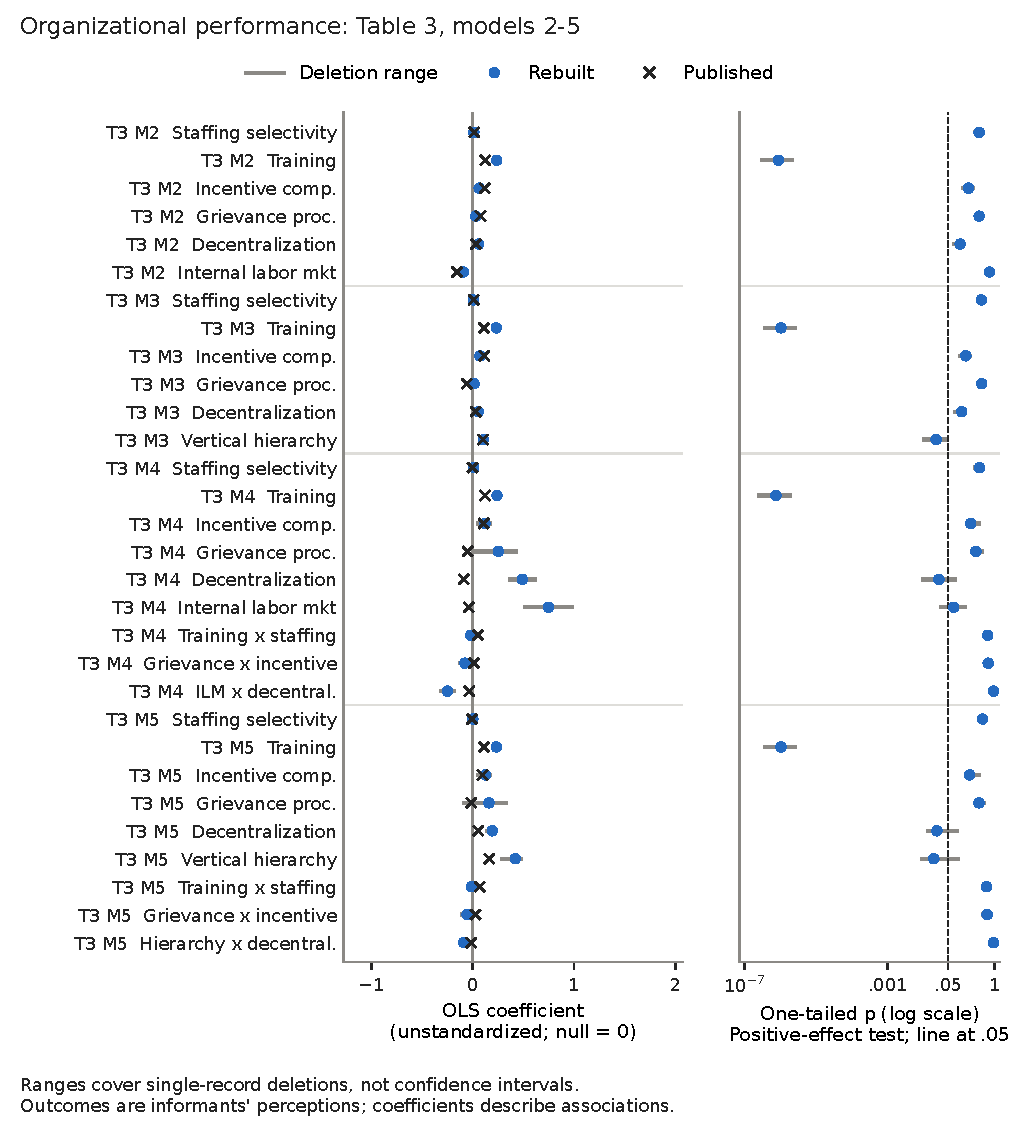
\includegraphics[width=\linewidth]{supplement_assets/delaney1996_organizational.pdf}\caption{Organizational performance: every HRM-practice and interaction coefficient in Table 3 models 2--5 (left; unstandardized OLS, null 0) and rebuilt one-tailed $p$-values (right, log scale). Lines show leave-one-record-out ranges, not confidence intervals ($N=361$ rebuilt, 590 published). Source: \artifact{studies/delaney1996/reports/figures/reconstruction_influence.csv}.}\label{fig:delaney1996}\end{figure}
\begin{figure}[p]\centering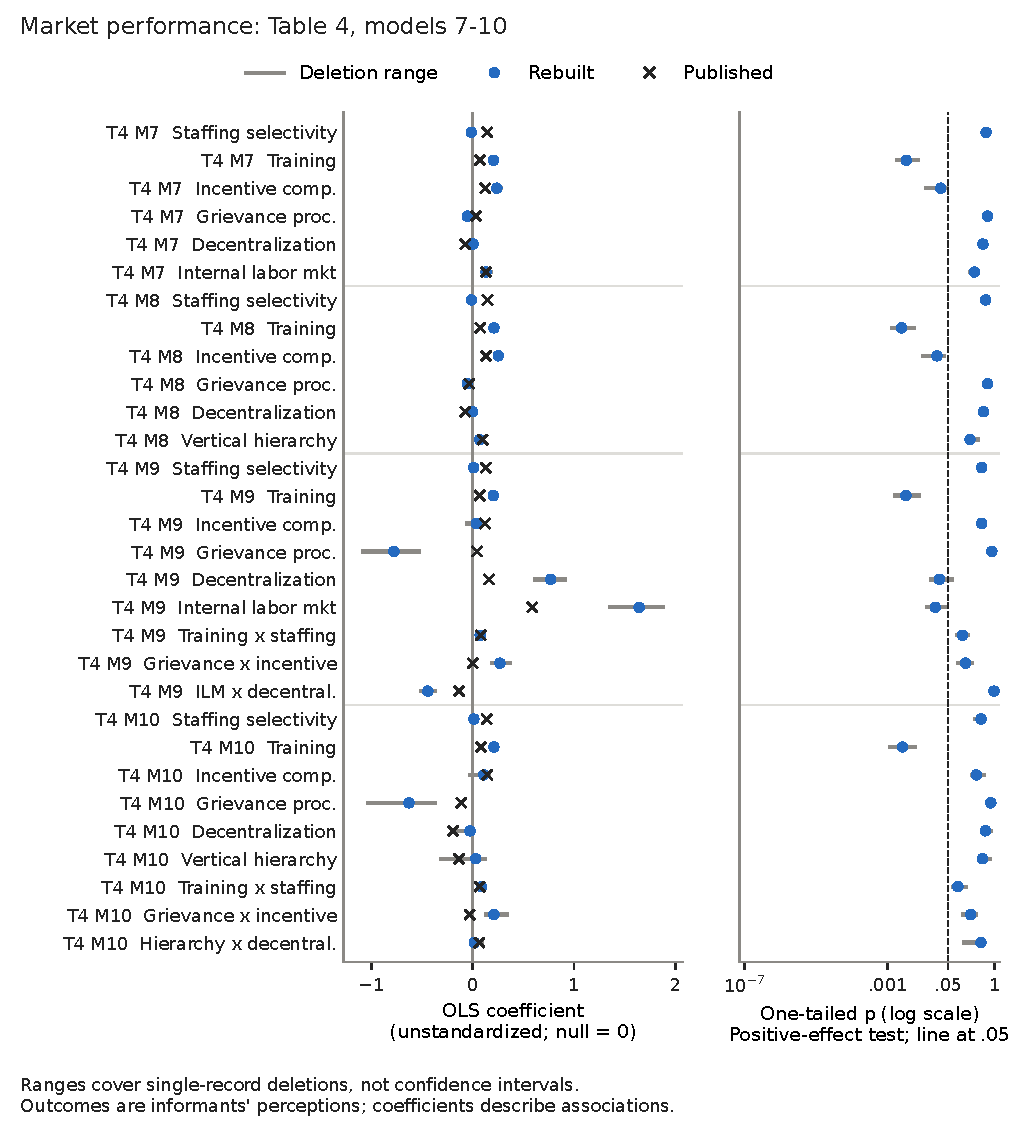
\includegraphics[width=\linewidth]{supplement_assets/delaney1996_market.pdf}\caption{Market performance: every HRM-practice and interaction coefficient in Table 4 models 7--10, with the same axes and symbols as Figure~\ref{fig:delaney1996}. Lines show leave-one-record-out ranges, not confidence intervals ($N=239$ rebuilt, 373 published). Source: \artifact{studies/delaney1996/reports/figures/reconstruction_influence.csv}.}\label{fig:delaney1996-market}\end{figure}

\textbf{Audit and unresolved record.} The scorer flagged 23 discrepancy candidates. The adversarial review overturned 16, left 7 uncertain and recommends confirming none: the incentive-compensation flags arise because the rebuilt SE is 1.5 times the published one; the staffing gap appears to come from construction rather than an article error; the subsidiary coefficient was coded in the opposite direction in the article's Table 2; and seven cells were flagged only because a near-zero estimate changed sign. The review traced most of the sample shortfall to three missing-data rules the article does not document: staffing items skipped for establishments that did not hire from outside, managers in the same occupation as the core group, and competition coded ``not applicable'', mostly for nonprofits. One gap is our own: Reader A's coding of the share of managers, which keeps those establishments, was logged as an origin in reconciliation but never executed, and no amended run was made. A post hoc exploration relaxing the three rules reaches $N=584$ and 373 and moves several estimates toward the printed ones (organizational incentive compensation 0.120; market staffing 0.119 to 0.122). It was found after seeing results, partly by matching sample size, so it is reported as a diagnostic and changes no classification.

Both readers found contradictions within the article (firm age described in years but labelled as logged; a 1--4 competition scale with mean .44 and SD .50; training ``standardized and averaged'' in the text but ``logged'' in a footnote), and the journal scan and the author's retypeset copy disagree on several cells. In sealed probes, both reader models recalled the data source and the 590-organization sample.

\textbf{Evidence.} \artifact{studies/delaney1996/reports/replication_report.md}, \artifact{reports/technical_supplement.md}, \artifact{reports/data/claim_cell_comparisons.csv}, \artifact{reports/data/claim_and_paper_outcomes.json}, \artifact{checks/audit/adversarial_v1/REVIEW.md}, \artifact{checks/scoring_rules_v1.json}, and \artifact{reconciliation/decisions_v1.md}. Full comparisons appear in Section~\ref{sec:tables-delaney1996}.

\clearpage
\section{Validation, artifact access, and reuse}\label{sec:reuse}
\subsection{Artifact map and commands}
\begin{table}[H]\centering\small
\begin{tabularx}{\linewidth}{@{}p{.40\linewidth}Y@{}}\toprule
Path & Contents\\\midrule
\artifact{CLAUDE.md}, \artifact{instructions/}, \artifact{prompts/} & Coordinator protocol, role prompts, reconciliation rules, scoring rules, and reporting standards.\\
\artifact{config/roles.json} & Pinned model and effort settings for each pipeline role.\\
\artifact{papers/catalog.json} & Article DOIs, file names, and SHA-256 checksums (PDFs omitted for copyright).\\
\artifact{papers/screening/} & Screening frame (11,051 records), full-text assessments (776), candidate lists (277 and 154), and methods.\\
\artifact{studies/<id>/reports/} & Replication report, technical supplement, common-rule report, influence figures, and CSV exports.\\
\artifact{studies/<id>/registry/} & Data provider URLs, release dates, SHA-256 hashes, and lineage records (raw data omitted).\\
\artifact{studies/<id>/reconciliation/} & Merged specifications, uncertain grids, and coordinator decision ledgers.\\
\artifact{studies/<id>/implementation/}, \artifact{runs/} & Implementer scripts in R, Python, and Julia, saved parameter outputs, and execution logs.\\
\artifact{studies/<id>/checks/}, \artifact{audits/} & Pre-run checker outputs, AI adversarial reviews, and adjudication records.\\
\artifact{studies/score_common.py} & Script that rescores all six studies under \artifact{studies/scoring_rules_common_v1.json}.\\\bottomrule
\end{tabularx}\caption{Directory map of the accompanying \artifact{Replication_management/} artifact.}\label{tab:artifact-map}\end{table}

Paths in the table are relative to \artifact{Replication_management/}. Conversation transcripts are omitted from this distribution; numerical outputs, execution logs, and written review records are retained. Historical receipts describe the original runs, before this anonymization.\par
To regenerate all cross-study common-rule tables and study summaries from the saved estimates:
\begin{quote}\small\ttfamily
cd Replication\_management/studies \&\& python score\_common.py
\end{quote}
Running this command with Python (\texttt{pandas} and \texttt{numpy}) reproduces all 26 common-rule summary files byte for byte. The script \artifact{proposal/scripts/build_supplement_assets.py} builds the LaTeX comparison tables in this document directly from those saved exports, and \artifact{proposal/} holds the sources of this supplement and the proposal.

\subsection{What has and has not been validated}
\begin{table}[H]\centering\small
\begin{tabularx}{\linewidth}{@{}p{.27\linewidth}Y@{}}\toprule
Check & Current status across the six studies\\\midrule
Independent implementations & Completed across 3 implementations in 5 studies (A and B in R, C in Python); Th\'ebaud completed A and B in R.\\
Data-loader verification & SHA-256 checksums, independent R/Python reads, and sample-count traces logged in each study's registry.\\
Synthetic scorer tests & Verified on synthetic test cases (including 8 unit tests in Lehman); empirical false-flag rate will be calibrated in Stage 2.\\
Memorization probes & Sealed title/author probes run for all 6 studies; Twenge readers recalled headline $d=0.57$ and Delaney readers the 590-organization sample, while the other 4 recalled no estimates.\\
Adversarial review & Completed on all flagged candidates using Anthropic and OpenAI models; third-family review planned for Stage 2.\\
Common-rule rescoring & Verified byte-for-byte via \artifact{score_common.py} across all 733 target terms.\\\bottomrule
\end{tabularx}\caption{Summary of completed verification steps and Stage 2 calibration tasks.}\end{table}

\subsection{Access routes for full reconstruction}
\begin{table}[H]\centering\small
\begin{tabularx}{\linewidth}{@{}lYY@{}}\toprule
Study & Data provider and access route & Main source-vintage difference\\\midrule
Lehman & Public download: nflverse play-by-play and schedule releases (2000--2005) & Two 2000-season games absent from public archive ($21,540$ vs $22,603$ plays).\\
Holderness & Public download: U.S.\ National Archives RG 389 (NAID 1263907) and RG 64 (NAID 1263923); GeoNames & Report month used in place of unarchived capture date ($100,672$ vs $100,464$).\\
Deephouse & Public download: Chicago Fed Call Reports (1983--1993), FDIC BankFind, FRED/BLS, Census/OMB & Metropolitan county filter yields $1,260 / 1,255$ bank-years vs $960$ published.\\
Th\'ebaud & Free ICPSR registration (\texttt{ICPSR\_20320} v6) plus public OECD, CEPR, ILO, UNDP, and World Bank series & Harmonized GEM v6 release and OECD early-education series differ from original vintage.\\
Twenge & Free ICPSR registration (\texttt{ICPSR\_07927} v4, \texttt{ICPSR\_09871} v1, \texttt{ICPSR\_20022} v3) & Public MTF files omit school/PSU cluster IDs and apply confidentiality weight top-coding.\\
Delaney & Free ICPSR registration (\texttt{ICPSR\_06240} v1) plus the Census Bureau's 1980 industry list & Same public release; three undocumented missing-data rules leave 361/239 vs 590/373 establishments; the authors' 33-group industry coding is unknown.\\\bottomrule
\end{tabularx}\caption{Data sources and access routes required to rerun the six studies from raw data.}\end{table}
Because publisher copyrights and ICPSR terms of use prohibit redistributing article PDFs and raw survey microdata, those files are omitted from \artifact{Replication_management/}. Each study's \artifact{README.md} and \artifact{registry/} folder list the exact filenames and SHA-256 hashes needed to verify a fresh download.

\subsection{Starting a new paper}
To run the pipeline on a new study, create a fresh \artifact{studies/<study_id>/} directory from the setup guide in \artifact{instructions/new_study.md}, register the article PDF hash in \artifact{papers/catalog.json}, and open an isolated coordinator session following \artifact{CLAUDE.md} and \artifact{instructions/workflow.md}.

\clearpage
\section{Complete numerical comparisons}\label{sec:comparisons}
The tables below report all 733 target terms in the common-rule scope (752 rows with Deephouse's two reader origins shown separately). An asterisk (\texttt{*}) marks a focal term under \texttt{common\_v1}. Published standard errors and significance stars are shown where printed in the article; reconstructed standard errors appear where exported by the study scorer, and native two-sided $p$-values are shown otherwise (\texttt{--} indicates that a quantity was not printed or not exported). In Lehman Table 5, log-odds coefficients are exponentiated to odds ratios for side-by-side display, while standardized distances $d_j$ and $p$-values are evaluated on the log-odds scale. Delaney's $p$-values are one-tailed (upper tail), as in the article.

Outcome codes: \texttt{C} = consistent on assessed criteria; \texttt{I} = indeterminate; \texttt{U} = unverified mismatch candidate; \texttt{FI} = fragile inference; \texttt{NA} = not assessed.

\subsection{Lehman et al.}\label{sec:tables-lehman2011}
{\scriptsize\setlength{\tabcolsep}{3pt}\renewcommand{\arraystretch}{1.06}
\begin{longtable}{@{}p{.245\linewidth}p{.17\linewidth}p{.17\linewidth}p{.085\linewidth}p{.060\linewidth}p{.08\linewidth}p{.07\linewidth}@{}}
\caption{Lehman et al.: all numerical targets in the common-rule scope}\label{tab:all:lehman2011}\\
\toprule Target & Published (SE) & Rebuilt (SE) & Native $p$ & $d$ & Study & Common\\\midrule
\endfirsthead\multicolumn{7}{l}{\small Lehman et al.: all numerical targets in the common-rule scope (continued)}\\\toprule Target & Published (SE) & Rebuilt (SE) & Native $p$ & $d$ & Study & Common\\\midrule\endhead\bottomrule\endfoot
M1: home field & 1.019 (0.049) & 1.004 & 0.9365 & 0.2948 & C & C\\
M1: minutes remaining & 0.946 (2.0e-03) ** & 0.9443 & 4.3e-175 & 0.4646 & C & C\\
M1: same conference & 1.008 (0.05) & 0.916 & 0.1934 & 1.9 & U & I\\
M1: same division & 0.969 (0.054) & 1.115 & 0.06578 & 2.488 & U & I\\
M1: total points & 0.941 (3.0e-03) ** & 0.9399 & 1.4e-60 & 0.1695 & C & C\\
M1: week & 1.02 (5.0e-03) ** & 1.021 & 5.5e-05 & 0.03733 & C & C\\
M1: yards first down & 0.826 (6.0e-03) ** & 0.8144 & 2.3e-168 & 1.72 & I & I\\
M1: yards touchdown & 0.976 (1.0e-03) ** & 0.9735 & 6.2e-141 & 1.312 & C & C\\
M2: below indicator & 1.12 (0.11) & 1.185 & 0.1032 & 0.5642 & C & C\\
M2: home field & 1.177 (0.059) ** & 1.14 & 0.01225 & 0.6276 & C & I\\
M2: minutes remaining & 0.975 (2.0e-03) ** & 0.9733 & 1.6e-27 & 0.4982 & C & C\\
M2: perf above * & 0.994 (7.0e-03) & 0.9924 & 0.3343 & 0.1427 & C & C\\
M2: perf below * & 0.883 (8.0e-03) ** & 0.8852 & 3.4e-33 & 0.1986 & C & C\\
M2: perf below sq * & 0.999 (0) ** & 0.9988 & 1.6e-04 & 0 & C & C\\
M2: same conference & 0.997 (0.051) & 0.9772 & 0.7404 & 0.3794 & C & C\\
M2: same division & 1.025 (0.059) & 1.095 & 0.1355 & 1.135 & C & C\\
M2: total points & 1.007 (5.0e-03) & 1.008 & 0.123 & 0.1706 & C & C\\
M2: week & 1.023 (5.0e-03) ** & 1.023 & 1.2e-05 & 0 & C & C\\
M2: yards first down & 0.813 (6.0e-03) ** & 0.8012 & 2.2e-180 & 1.755 & I & I\\
M2: yards touchdown & 0.973 (1.0e-03) ** & 0.9706 & 8.5e-157 & 1.24 & C & C\\
M3: below indicator & 0.857 (0.092) & 0.8569 & 0.1757 & 0 & C & C\\
M3: home field & 1.167 (0.06) ** & 1.12 & 0.03442 & 0.7794 & C & I\\
M3: minutes remaining & 1.019 (3.0e-03) ** & 1.019 & 8.6e-08 & 0 & C & C\\
M3: perf above & 1.038 (0.01) ** & 1.038 & 1.2e-04 & 0 & C & C\\
M3: perf above x min * & 0.998 (0) ** & 0.9979 & 3.3e-06 & 0 & C & C\\
M3: perf below & 0.669 (0.012) ** & 0.6648 & 6.0e-106 & 0.2935 & C & C\\
M3: perf below sq & 0.993 (1.0e-03) ** & 0.9923 & 1.5e-42 & 0.1473 & C & C\\
M3: perf below sq x min * & 1 (0) ** & 1 & 7.0e-16 & 0 & C & C\\
M3: perf below x min * & 1.011 (1.0e-03) ** & 1.011 & 2.4e-57 & 0 & C & C\\
M3: same conference & 0.999 (0.052) & 0.9973 & 0.9695 & 0.02369 & C & C\\
M3: same division & 1.046 (0.062) & 1.105 & 0.1121 & 0.9052 & C & C\\
M3: total points & 1.014 (5.0e-03) ** & 1.015 & 9.0e-03 & 0.1037 & C & C\\
M3: week & 1.026 (5.0e-03) ** & 1.027 & 9.5e-07 & 0.0468 & C & C\\
M3: yards first down & 0.801 (6.0e-03) ** & 0.7881 & 2.8e-188 & 1.921 & I & I\\
M3: yards touchdown & 0.972 (1.0e-03) ** & 0.9697 & 8.4e-157 & 1.202 & C & C\\
all: gap-14 & -3.9e-03 (5.0e-04) ** & -9.6e-03 & 1.1e-08 & 10.29 & U & U\\
all: gap-28 & -4.4e-03 (2.8e-03) & -0.01148 & 2.2e-06 & 2.468 & U & I\\
all: gap-42 & -2.6e-03 (6.2e-03) & -5.9e-03 & 0.1769 & 0.5221 & C & C\\
all: gap0 & -2.2e-03 (3.0e-04) ** & -3.6e-03 & 8.6e-08 & 3.961 & U & U\\
all: gap14 & -6.0e-04 (2.0e-04) ** & -1.7e-04 & 0.3069 & 1.502 & U & U\\
all: gap28 & -4.0e-04 (1.0e-04) ** & -1.6e-04 & 0.2528 & 1.282 & U & U\\
all: gap42 & -3.0e-04 (0) ** & -1.4e-04 & 0.1939 & 2.153 & U & U\\
q1: gap-14 & 4.0e-04 (1.0e-04) ** & 1.1e-03 & 0.01361 & 4.56 & U & U\\
q1: gap-28 & -1.1e-03 (9.0e-04) & -3.5e-03 & 0.2544 & 2.493 & I & I\\
q1: gap-42 & -0.0163 (0.0213) & -0.04241 & 0.2768 & 1.22 & C & C\\
q1: gap0 & 6.6e-03 (1.4e-03) ** & 0.01701 & 2.4e-04 & 7.148 & U & U\\
q1: gap14 & -1.3e-03 (2.0e-04) ** & -3.6e-03 & 1.1e-05 & 8.966 & U & U\\
q1: gap28 & -5.0e-04 (1.0e-04) ** & -1.3e-03 & 6.0e-04 & 5.239 & U & U\\
q1: gap42 & -2.0e-04 (1.0e-04) * & -4.8e-04 & 0.06033 & 1.507 & I & I\\
q2: gap-14 & -9.0e-04 (3.0e-04) * & -2.4e-03 & 0.02141 & 4.099 & U & U\\
q2: gap-28 & -3.1e-03 (2.2e-03) & -7.9e-03 & 0.1482 & 2.098 & I & I\\
q2: gap-42 & -9.9e-03 (0.0111) & -0.01977 & 0.2189 & 0.8808 & C & C\\
q2: gap0 & 1.0e-04 (5.0e-04) & 3.5e-04 & 0.8111 & 0.3612 & C & C\\
q2: gap14 & -9.0e-04 (2.0e-04) ** & -2.4e-03 & 2.3e-04 & 5.797 & U & U\\
q2: gap28 & -5.0e-04 (0) ** & -1.4e-03 & 3.1e-08 & 16.57 & U & U\\
q2: gap42 & -3.0e-04 (1.0e-04) ** & -7.7e-04 & 1.2e-04 & 2.82 & I & I\\
q3: gap-14 & -9.8e-03 (8.0e-04) ** & -0.01908 & 1.3e-17 & 10.86 & U & U\\
q3: gap-28 & -4.7e-03 (2.8e-03) + & -5.9e-03 & 0.1178 & 0.4184 & C & I\\
q3: gap-42 & 6.8e-03 (3.1e-03) * & 0.0108 & 0.09502 & 1.254 & C & I\\
q3: gap0 & -3.6e-03 (2.0e-04) ** & -0.01017 & 5.3e-09 & 26.09 & U & U\\
q3: gap14 & -3.0e-04 (2.0e-04) & -7.4e-04 & 0.1821 & 1.542 & I & I\\
q3: gap28 & -2.0e-04 (1.0e-04) + & -6.4e-04 & 0.1155 & 2.592 & I & I\\
q3: gap42 & -2.0e-04 (1.0e-04) * & -5.5e-04 & 0.05379 & 2.022 & I & I\\
q4: gap-14 & -0.0352 (1.6e-03) ** & -0.03711 & 2.5e-105 & 1.126 & C & C\\
q4: gap-28 & 2.0e-04 (2.6e-03) & 1.3e-03 & 0.472 & 0.3906 & C & C\\
q4: gap-42 & 0.0353 (2.0e-03) ** & 0.04287 & 5.5e-10 & 3.67 & U & U\\
q4: gap0 & -5.5e-03 (4.0e-04) ** & -0.0161 & 9.2e-11 & 23.44 & U & U\\
q4: gap14 & 5.0e-04 (2.0e-04) * & 1.5e-03 & 0.04257 & 3.791 & U & U\\
q4: gap28 & 6.0e-04 (4.0e-04) + & 1.9e-03 & 0.08255 & 2.759 & I & I\\
q4: gap42 & 8.0e-04 (6.0e-04) & 2.4e-03 & 0.1211 & 2.313 & I & I\\
\end{longtable}}

\clearpage
\subsection{Holderness and Pontiff}\label{sec:tables-holderness2012}
{\scriptsize\setlength{\tabcolsep}{3pt}\renewcommand{\arraystretch}{1.06}
\begin{longtable}{@{}p{.245\linewidth}p{.17\linewidth}p{.17\linewidth}p{.085\linewidth}p{.060\linewidth}p{.08\linewidth}p{.07\linewidth}@{}}
\caption{Holderness and Pontiff: all numerical targets in the common-rule scope}\label{tab:all:holderness2012}\\
\toprule Target & Published (SE) & Rebuilt (SE) & Native $p$ & $d$ & Study & Common\\\midrule
\endfirsthead\multicolumn{7}{l}{\small Holderness and Pontiff: all numerical targets in the common-rule scope (continued)}\\\toprule Target & Published (SE) & Rebuilt (SE) & Native $p$ & $d$ & Study & Common\\\midrule\endhead\bottomrule\endfoot
T001 cap simple steepness * & -0.06 & -0.06354 & 8.4e-04 & -- & C & C\\
T003 cap full steepness * & -0.11 & -0.1034 & 1.7e-08 & -- & C & C\\
T004 cap full men & 0.09 & 0.07809 & 0.04362 & -- & C & C\\
T005 cap full men sq & 0 & -0.04549 & 0.2906 & -- & C & C\\
T006 cap full length & 0.01 & -1.0e-03 & 0.7045 & -- & I & C\\
T007 cap full height & -0.03 & -0.01926 & 0.1593 & -- & C & C\\
T008 cap full age & -0.08 & -0.08567 & 3.3e-04 & -- & C & C\\
T009 cap full education & -0.02 & -0.02075 & 5.2e-05 & -- & C & C\\
T010 cap full dependents & 0.02 & 0.01903 & 3.1e-03 & -- & C & C\\
T011 cap full officer & -0.04 & -0.03665 & 0.09787 & -- & C & C\\
T013 camp simple steepness * & -0.33 & -0.3693 & 0.03487 & -- & C & C\\
T014 camp simple japan & -0.22 & -0.2164 & 0.01109 & -- & C & I\\
T016 camp full steepness * & -0.18 & -0.1688 & 0.1447 & -- & C & C\\
T017 camp full japan & -0.13 & -0.1772 & 9.3e-03 & -- & C & C\\
T018 camp full men & 0.11 & -0.05817 & 0.794 & -- & I & C\\
T019 camp full men sq & 0 & 0.1047 & 0.5662 & -- & I & C\\
T020 camp full distance & -0.24 & -0.2304 & 7.6e-03 & -- & C & C\\
T021 camp full length & 0.06 & 4.6e-03 & 0.304 & -- & C & C\\
T022 camp full height & -0.02 & -0.01927 & 0.2431 & -- & C & C\\
T023 camp full age & -0.1 & -0.1059 & 5.6e-03 & -- & C & C\\
T024 camp full education & -0.02 & -0.02278 & 7.7e-03 & -- & C & C\\
T025 camp full dependents & 0.02 & 0.02471 & 8.5e-03 & -- & C & C\\
T026 camp full officer & -0.02 & -0.02552 & 0.2381 & -- & C & C\\
T028 cap simple sameness * & -0.03 & -0.0221 & 0.04723 & -- & C & C\\
T030 cap full sameness * & -0.07 & -0.06912 & 2.7e-10 & -- & C & C\\
T031 cap full men & 0.1 & 0.1002 & 0.01012 & -- & C & C\\
T032 cap full men sq & 0 & -0.06481 & 0.137 & -- & C & C\\
T033 cap full length & 0.01 & -6.9e-04 & 0.7998 & -- & I & C\\
T034 cap full height & -0.03 & -0.01934 & 0.1558 & -- & C & C\\
T035 cap full age & -0.08 & -0.08598 & 2.9e-04 & -- & C & C\\
T036 cap full education & -0.02 & -0.02093 & 4.2e-05 & -- & C & C\\
T037 cap full dependents & 0.02 & 0.01914 & 2.8e-03 & -- & C & C\\
T038 cap full officer & -0.04 & -0.0392 & 0.0817 & -- & C & I\\
T040 camp simple sameness * & -0.23 & -0.2419 & 8.6e-03 & -- & C & C\\
T041 camp simple japan & -0.24 & -0.2337 & 9.7e-04 & -- & C & C\\
T043 camp full sameness * & -0.18 & -0.1537 & 3.1e-03 & -- & C & C\\
T044 camp full japan & -0.1 & -0.1546 & 6.5e-03 & -- & C & C\\
T045 camp full men & 0.15 & -0.01039 & 0.9585 & -- & I & C\\
T046 camp full men sq & 0 & 0.06222 & 0.7056 & -- & I & C\\
T047 camp full distance & -0.23 & -0.2286 & 3.1e-03 & -- & C & C\\
T048 camp full length & 0.02 & 3.6e-03 & 0.3587 & -- & C & C\\
T049 camp full height & -0.02 & -0.01854 & 0.2266 & -- & C & C\\
T050 camp full age & -0.08 & -0.09636 & 3.1e-03 & -- & C & C\\
T051 camp full education & -0.02 & -0.02278 & 2.4e-03 & -- & C & C\\
T052 camp full dependents & 0.02 & 0.02345 & 5.4e-03 & -- & C & C\\
T053 camp full officer & -0.02 & -0.03379 & 0.1546 & -- & C & C\\
T056 cap simple steepness & -0.09 & -0.1105 & 3.5e-04 & -- & C & C\\
T057 cap simple sameness & 0.02 & 0.0351 & 0.04048 & -- & C & C\\
T058 cap full steepness & -0.04 & -0.05897 & 0.06262 & -- & C & C\\
T059 cap full sameness & -0.05 & -0.0383 & 0.04494 & -- & C & C\\
T060 camp simple steepness & -0.32 & -0.41 & 0.2508 & -- & C & C\\
T061 camp simple sameness & -0.01 & 0.03915 & 0.8425 & -- & I & C\\
T062 camp full steepness & 0.09 & 0.01523 & 0.9525 & -- & C & C\\
T063 camp full sameness & -0.24 & -0.1638 & 0.2439 & -- & C & I\\
T072 cap simple officer x hierarchy & -0.02 & -0.05682 & 0.2183 & -- & C & C\\
T073 cap simple steepness & -0.06 & -0.05912 & 3.2e-03 & -- & C & C\\
T074 cap simple officer & -0.02 & -0.01073 & 0.4381 & -- & C & C\\
T076 cap full officer x hierarchy & -0.04 & -0.06827 & 0.0652 & -- & C & C\\
T077 cap full steepness & -0.08 & -0.08983 & 7.5e-06 & -- & C & C\\
T078 cap full officer & -0.02 & -7.1e-03 & 0.6186 & -- & C & C\\
T079 cap full men & 0.09 & 0.08398 & 0.03031 & -- & C & C\\
T080 cap full men sq & 0 & -0.05067 & 0.2422 & -- & C & C\\
T081 cap full length & 0.01 & -6.5e-04 & 0.8076 & -- & I & C\\
T082 cap full height & -0.03 & -0.01935 & 0.1574 & -- & C & C\\
T083 cap full age & -0.08 & -0.08792 & 2.5e-04 & -- & C & C\\
T084 cap full education & -0.02 & -0.02056 & 6.1e-05 & -- & C & C\\
T085 cap full dependents & 0.02 & 0.01919 & 2.9e-03 & -- & C & C\\
T087 camp simple officer x hierarchy & -0.13 & -0.1192 & 0.2765 & -- & C & C\\
T088 camp simple steepness & -0.28 & -0.3406 & 0.06447 & -- & C & C\\
T089 camp simple officer & 0.01 & 8.6e-03 & 0.8011 & -- & C & C\\
T090 camp simple japan & -0.23 & -0.2217 & 0.01046 & -- & C & I\\
T092 camp full officer x hierarchy & -0.18 & -0.174 & 0.01441 & -- & C & I\\
T093 camp full steepness & -0.11 & -0.125 & 0.2711 & -- & C & C\\
T094 camp full officer & 0.03 & 0.02453 & 0.1498 & -- & C & I\\
T095 camp full japan & -0.14 & -0.1815 & 8.4e-03 & -- & C & C\\
T096 camp full men & 0.09 & -0.05316 & 0.8051 & -- & I & C\\
T097 camp full men sq & 0 & 0.1011 & 0.5673 & -- & C & C\\
T098 camp full distance & -0.23 & -0.2297 & 5.6e-03 & -- & C & C\\
T099 camp full length & 0.07 & 5.1e-03 & 0.2633 & -- & C & C\\
T100 camp full height & -0.02 & -0.01908 & 0.2354 & -- & C & C\\
T101 camp full age & -0.1 & -0.1118 & 3.0e-03 & -- & C & C\\
T102 camp full education & -0.01 & -0.02114 & 0.01406 & -- & C & C\\
T103 camp full dependents & 0.02 & 0.02464 & 6.8e-03 & -- & C & C\\
T105 cap simple officer x hierarchy & -0.05 & -0.05116 & 0.04627 & -- & C & C\\
T106 cap simple sameness & -0.01 & -0.01506 & 0.2766 & -- & C & C\\
T107 cap simple officer & 0.01 & 0.0158 & 0.179 & -- & C & C\\
T109 cap full officer x hierarchy & -0.04 & -0.04393 & 0.03852 & -- & C & C\\
T110 cap full sameness & -0.04 & -0.04818 & 5.2e-04 & -- & C & C\\
T111 cap full officer & 0.01 & 0.0101 & 0.3851 & -- & C & C\\
T112 cap full men & 0.11 & 0.09761 & 0.01259 & -- & C & I\\
T113 cap full men sq & 0 & -0.06329 & 0.1483 & -- & C & C\\
T114 cap full length & 0.01 & -7.9e-04 & 0.7733 & -- & I & C\\
T115 cap full height & -0.03 & -0.01944 & 0.1539 & -- & C & C\\
T116 cap full age & -0.08 & -0.08816 & 2.3e-04 & -- & C & C\\
T117 cap full education & -0.02 & -0.02073 & 4.9e-05 & -- & C & C\\
T118 cap full dependents & 0.02 & 0.01928 & 2.6e-03 & -- & C & C\\
T120 camp simple officer x hierarchy & -0.06 & -0.07476 & 0.2913 & -- & C & C\\
T121 camp simple sameness & -0.22 & -0.2387 & 0.02301 & -- & C & C\\
T122 camp simple officer & 0.02 & 0.02548 & 0.5918 & -- & C & C\\
T123 camp simple japan & -0.23 & -0.2315 & 1.4e-03 & -- & C & C\\
T125 camp full officer x hierarchy & -0.08 & -0.09035 & 0.01549 & -- & C & C\\
T126 camp full sameness & -0.14 & -0.1224 & 0.01249 & -- & C & C\\
T127 camp full officer & 0.03 & 0.03639 & 0.01595 & -- & C & C\\
T128 camp full japan & -0.1 & -0.158 & 5.1e-03 & -- & C & C\\
T129 camp full men & 0.13 & -9.7e-03 & 0.9608 & -- & I & C\\
T130 camp full men sq & 0 & 0.06275 & 0.7006 & -- & I & C\\
T131 camp full distance & -0.21 & -0.2294 & 2.5e-03 & -- & C & C\\
T132 camp full length & 0.03 & 3.7e-03 & 0.3432 & -- & C & C\\
T133 camp full height & -0.02 & -0.0186 & 0.2217 & -- & C & C\\
T134 camp full age & -0.08 & -0.1014 & 1.8e-03 & -- & C & C\\
T135 camp full education & -0.01 & -0.02197 & 4.0e-03 & -- & C & C\\
T136 camp full dependents & 0.02 & 0.02362 & 4.7e-03 & -- & C & C\\
\end{longtable}}

\clearpage
\subsection{Deephouse}\label{sec:tables-deephouse1999}
{\scriptsize\setlength{\tabcolsep}{3pt}\renewcommand{\arraystretch}{1.06}
\begin{longtable}{@{}p{.245\linewidth}p{.17\linewidth}p{.17\linewidth}p{.085\linewidth}p{.060\linewidth}p{.08\linewidth}p{.07\linewidth}@{}}
\caption{Deephouse: all numerical targets in the common-rule scope}\label{tab:all:deephouse1999}\\
\toprule Target & Published (SE) & Rebuilt (SE) & Native $p$ & $d$ & Study & Common\\\midrule
\endfirsthead\multicolumn{7}{l}{\small Deephouse: all numerical targets in the common-rule scope (continued)}\\\toprule Target & Published (SE) & Rebuilt (SE) & Native $p$ & $d$ & Study & Common\\\midrule\endhead\bottomrule\endfoot
M1 intercept [O\_A] & 0.929 (0.169) *** & 0.8389 (0.1095) & 3.7e-14 & 0.5286 & C & I\\
M1 intercept [O\_B] & 0.929 (0.169) *** & 0.8726 (0.1089) & 2.5e-15 & 0.3298 & C & I\\
M1 MS [O\_A] & -0.576 (0.138) *** & -0.574 (0.1275) & 7.3e-06 & 0.0111 & C & I\\
M1 MS [O\_B] & -0.576 (0.138) *** & -0.7187 (0.1178) & 1.4e-09 & 1.027 & C & I\\
M1 TER [O\_A] & -9.948 (2.001) *** & -9.002 (1.26) & 1.5e-12 & 0.4725 & C & I\\
M1 TER [O\_B] & -9.948 (2.001) *** & -9.027 (1.255) & 1.1e-12 & 0.4598 & C & I\\
M1 RMG [O\_A] & 0.014 (4.0e-03) *** & 6.7e-03 (3.6e-03) & 0.06537 & 1.505 & U & I\\
M1 RMG [O\_B] & 0.014 (4.0e-03) *** & 9.9e-03 (3.3e-03) & 2.5e-03 & 0.8078 & C & I\\
M1 lag [O\_A] & 0.369 (0.028) *** & 0.3994 (0.02151) & 3.4e-68 & 1.05 & C & I\\
M1 lag [O\_B] & 0.369 (0.028) *** & 0.3915 (0.02181) & 2.9e-64 & 0.7709 & C & I\\
M2 intercept [O\_A] & 1.164 (0.172) *** & 0.9233 (0.1106) & 1.8e-16 & 1.393 & C & I\\
M2 intercept [O\_B] & 1.164 (0.172) *** & 0.9064 (0.1106) & 6.0e-16 & 1.49 & C & I\\
M2 SD [O\_A] * & -0.02 (4.0e-03) *** & -0.01402 (3.3e-03) & 2.2e-05 & 1.217 & C & I\\
M2 SD [O\_B] * & -0.02 (4.0e-03) *** & -6.1e-03 (3.6e-03) & 0.08762 & 2.971 & U & I\\
M2 MS [O\_A] & -0.093 (0.161) & -0.1824 (0.1564) & 0.2436 & 0.5507 & C & I\\
M2 MS [O\_B] & -0.093 (0.161) & -0.5848 (0.1414) & 3.8e-05 & 3.042 & U & I\\
M2 TER [O\_A] & -10.6 (1.974) *** & -8.615 (1.255) & 1.0e-11 & 1.006 & C & I\\
M2 TER [O\_B] & -10.6 (1.974) *** & -8.805 (1.261) & 4.7e-12 & 0.9094 & C & I\\
M2 RMG [O\_A] & 0.016 (4.0e-03) *** & 9.2e-03 (3.7e-03) & 0.01199 & 1.392 & I & I\\
M2 RMG [O\_B] & 0.016 (4.0e-03) *** & 0.01053 (3.3e-03) & 1.3e-03 & 1.104 & C & I\\
M2 lag [O\_A] & 0.361 (0.027) *** & 0.3996 (0.02136) & 4.9e-69 & 1.384 & C & I\\
M2 lag [O\_B] & 0.361 (0.027) *** & 0.3917 (0.02179) & 2.0e-64 & 1.099 & C & I\\
M3 intercept [O\_A] & 0.511 (0.171) ** & 0.02531 (0.1533) & 0.8688 & 2.829 & U & I\\
M3 intercept [O\_B] & 0.511 (0.171) ** & 0.2288 (0.1555) & 0.1414 & 1.642 & U & I\\
M3 SD2 [O\_A] * & -6.0e-03 (1.0e-03) *** & -4.3e-03 (5.2e-04) & 4.5e-16 & 0.8056 & C & I\\
M3 SD2 [O\_B] * & -6.0e-03 (1.0e-03) *** & -3.9e-03 (6.4e-04) & 1.3e-09 & 1.046 & C & I\\
M3 SD [O\_A] * & 0.17 (0.017) *** & 0.1116 (0.01559) & 1.4e-12 & 3.306 & U & I\\
M3 SD [O\_B] * & 0.17 (0.017) *** & 0.1003 (0.01777) & 2.1e-08 & 3.954 & U & I\\
M3 MS [O\_A] & -0.457 (0.155) ** & -0.3806 (0.1543) & 0.01376 & 0.4884 & I & I\\
M3 MS [O\_B] & -0.457 (0.155) ** & -0.7714 (0.1427) & 7.7e-08 & 2.019 & I & I\\
M3 TER [O\_A] & -15.39 (1.895) *** & -5.93 (1.265) & 3.1e-06 & 4.989 & U & I\\
M3 TER [O\_B] & -15.39 (1.895) *** & -7.121 (1.273) & 2.7e-08 & 4.361 & U & I\\
M3 RMG [O\_A] & 0.018 (3.0e-03) *** & 7.0e-03 (3.6e-03) & 0.05188 & 3.005 & U & I\\
M3 RMG [O\_B] & 0.018 (3.0e-03) *** & 0.0105 (3.2e-03) & 1.2e-03 & 1.999 & I & I\\
M3 lag [O\_A] & 0.403 (0.026) *** & 0.4657 (0.02231) & 2.9e-83 & 2.348 & I & I\\
M3 lag [O\_B] & 0.403 (0.026) *** & 0.4287 (0.02232) & 3.1e-72 & 0.9498 & C & I\\
M3 SQ SD2 [O\_A] & -1.0e-03 (1.0e-04) text: negative and significant (mapped to p<.05) & -6.4e-04 (1.1e-04) & 5.9e-09 & 0 & C & I\\
M3 SQ SD2 [O\_B] & -1.0e-03 (1.0e-04) text: negative and significant (mapped to p<.05) & -3.7e-04 (1.3e-04) & 4.0e-03 & 0.8458 & C & I\\
\end{longtable}}

\clearpage
\subsection{Th\'ebaud}\label{sec:tables-thebaud2015}
{\scriptsize\setlength{\tabcolsep}{3pt}\renewcommand{\arraystretch}{1.06}
\begin{longtable}{@{}p{.245\linewidth}p{.17\linewidth}p{.17\linewidth}p{.085\linewidth}p{.060\linewidth}p{.08\linewidth}p{.07\linewidth}@{}}
\caption{Thébaud: all numerical targets in the common-rule scope}\label{tab:all:thebaud2015}\\
\toprule Target & Published (SE) & Rebuilt (SE) & Native $p$ & $d$ & Study & Common\\\midrule
\endfirsthead\multicolumn{7}{l}{\small Thébaud: all numerical targets in the common-rule scope (continued)}\\\toprule Target & Published (SE) & Rebuilt (SE) & Native $p$ & $d$ & Study & Common\\\midrule\endhead\bottomrule\endfoot
M1 year2002 & 0.05 (0.08) & -0.02545 (0.05773) & 0.6593 & 0.8806 & I & C\\
M1 year2003 & 0.01 (0.08) & 0.05693 (0.05771) & 0.3239 & 0.5242 & C & C\\
M1 year2004 & 0.13 (0.08) • & 0.02323 (0.05724) & 0.6849 & 1.272 & C & I\\
M1 year2005 & 0.2 (0.08) •• & 0.04414 (0.05783) & 0.4453 & 1.886 & U & U\\
M1 year2006 & 0.04 (0.08) & -0.0228 (0.05839) & 0.6962 & 0.7225 & I & C\\
M1 year2007 & 0.07 (0.08) & 0.05413 (0.05977) & 0.3651 & 0.1358 & C & C\\
M1 year2008 & 0.2 (0.09) •• & 0.04332 (0.06132) & 0.4799 & 1.685 & U & U\\
M1 age c & 0.02 (1.0e-03) ••• & 0.01963 (5.3e-04) & 0 & 0 & C & C\\
M1 age c2 & -1.0e-03 (1.0e-04) ••• & -1.3e-03 (5.6e-05) & 0 & 0 & C & C\\
M1 female & -0.57 (0.04) ••• & -0.5624 (0.04168) & 0 & 0.06423 & C & C\\
M1 (Intercept) & -1.63 (0.1) ••• & -1.185 (0.09041) & 0 & 4.396 & U & U\\
M1 postsecondary & 0.04 (0.01) ••• & 0.02606 (9.8e-03) & 7.7e-03 & 0.8944 & FI & C\\
M2 year2002 & 0.11 (0.08) & 0.02981 (0.06289) & 0.6356 & 0.9399 & C & C\\
M2 year2003 & 0.06 (0.08) & 0.103 (0.06576) & 0.1174 & 0.4747 & C & C\\
M2 year2004 & 0.09 (0.08) & 0.0788 (0.07315) & 0.2814 & 0.07751 & C & C\\
M2 year2005 & 0.24 (0.09) ••• & 0.1172 (0.07664) & 0.1262 & 1.309 & U & U\\
M2 year2006 & 0.08 (0.09) & 0.07112 (0.0876) & 0.4168 & 0.04306 & C & C\\
M2 year2007 & 0.11 (0.09) & 0.1633 (0.09454) & 0.08404 & 0.537 & C & C\\
M2 year2008 & 0.18 (0.1) • & 0.1501 (0.1016) & 0.1393 & 0.2487 & C & I\\
M2 age c & 0.02 (1.0e-03) ••• & 0.01964 (5.3e-04) & 0 & 0 & C & C\\
M2 epl & -1.0e-03 (0.07) & -0.06492 (0.07186) & 0.3663 & 0.906 & C & C\\
M2 female & -0.57 (0.04) ••• & -0.5627 (0.04273) & 0 & 0.0578 & C & C\\
M2 fert & 0.09 (0.09) & 0.02875 (0.07097) & 0.6854 & 0.625 & C & C\\
M2 gdp & -0.2 (0.07) ••• & -0.09309 (0.06539) & 0.1545 & 1.456 & U & U\\
M2 (Intercept) & -1.65 (0.09) ••• & -1.287 (0.09873) & 0 & 3.976 & U & U\\
M2 leave & -0.13 (0.13) & -0.1202 (0.04943) & 0.01504 & 0.03704 & C & C\\
M2 leave sq & 0.18 (0.12) & 0.02313 (0.01358) & 0.08843 & 1.266 & C & C\\
M2 wmgr & 0.01 (0.06) & 9.6e-03 (0.03895) & 0.8053 & 0 & C & C\\
M2 postsecondary & 0.04 (0.01) ••• & 0.02354 (9.8e-03) & 0.01642 & 1.146 & FI & I\\
M2 status & 0.18 (0.04) ••• & 0.06752 (0.03026) & 0.02564 & 2.687 & I & I\\
M2 childcare & 0.04 (0.06) & -0.02458 (0.069) & 0.7216 & 0.993 & I & C\\
M2 unemp & -0.08 (0.06) & 2.1e-03 (0.04722) & 0.965 & 1.285 & I & C\\
M2 parttime & 0.03 (0.07) & -0.03573 (0.06678) & 0.5926 & 0.8676 & I & C\\
M3 year2002 & 0.11 (0.08) & 0.03013 (0.06292) & 0.6321 & 0.9359 & C & C\\
M3 year2003 & 0.07 (0.08) & 0.1035 (0.06579) & 0.1157 & 0.3559 & C & C\\
M3 year2004 & 0.1 (0.08) & 0.07972 (0.07316) & 0.2758 & 0.191 & C & C\\
M3 year2005 & 0.25 (0.09) ••• & 0.1194 (0.07663) & 0.1192 & 1.395 & U & U\\
M3 year2006 & 0.09 (0.09) & 0.07478 (0.08757) & 0.3932 & 0.1136 & C & C\\
M3 year2007 & 0.13 (0.09) & 0.1688 (0.09448) & 0.07406 & 0.3752 & C & C\\
M3 year2008 & 0.2 (0.1) •• & 0.156 (0.1015) & 0.1244 & 0.3904 & U & U\\
M3 age c & 0.02 (1.0e-03) ••• & 0.01964 (5.3e-04) & 0 & 0 & C & C\\
M3 age c2 & -1.0e-03 (1.0e-04) ••• & -1.3e-03 (5.7e-05) & 0 & 0 & C & C\\
M3 female x childcare * & -0.1 (0.04) ••• & -0.1308 (0.03353) & 9.6e-05 & 0.644 & C & C\\
M3 epl & -0.02 (0.07) & -0.06484 (0.07159) & 0.3651 & 0.5691 & C & C\\
M3 female & -0.58 (0.04) ••• & -0.5688 (0.03475) & 0 & 0.1541 & C & C\\
M3 fert & 0.07 (0.08) & 0.0268 (0.07087) & 0.7053 & 0.4775 & C & C\\
M3 gdp & -0.2 (0.07) ••• & -0.09553 (0.06529) & 0.1435 & 1.421 & U & U\\
M3 (Intercept) & -1.67 (0.09) ••• & -1.29 (0.0985) & 0 & 4.162 & U & U\\
M3 leave & -0.15 (0.13) & -0.121 (0.0499) & 0.01532 & 0.1847 & C & C\\
M3 leave sq & 0.18 (0.12) & 0.02479 (0.01383) & 0.07303 & 1.252 & C & C\\
M3 female x leave sq & 0.01 (0.08) & -5.1e-03 (0.01125) & 0.651 & 0.1261 & I & C\\
M3 female x leave & -0.05 (0.08) & -9.7e-03 (0.03199) & 0.7609 & 0.4408 & C & C\\
M3 female x parttime & -0.03 (0.04) & 7.0e-03 (0.03233) & 0.8287 & 0.7998 & I & C\\
M3 wmgr & 1.0e-03 (0.06) & 9.6e-03 (0.03894) & 0.8061 & 0.1343 & C & C\\
M3 postsecondary & 0.04 (0.01) ••• & 0.02366 (9.8e-03) & 0.01588 & 1.134 & FI & I\\
M3 status & 0.18 (0.04) ••• & 0.0678 (0.03025) & 0.02501 & 2.68 & I & I\\
M3 childcare & 0.04 (0.06) & -0.01137 (0.06896) & 0.869 & 0.7728 & I & C\\
M3 unemp & -0.08 (0.06) & 1.3e-03 (0.04721) & 0.9783 & 1.271 & I & C\\
M3 parttime & 0.03 (0.07) & -0.03719 (0.06664) & 0.5768 & 0.8884 & I & C\\
M4 year2002 & -0.04 (0.13) & -0.01998 (0.1416) & 0.8878 & 0.1156 & I & C\\
M4 year2003 & 4.0e-03 (0.13) & -0.02514 (0.1452) & 0.8625 & 0.2203 & I & C\\
M4 year2004 & -0.02 (0.12) & -0.2256 (0.1526) & 0.1392 & 1.672 & I & I\\
M4 year2005 & 0.16 (0.13) & 0.03878 (0.1593) & 0.8077 & 0.894 & I & C\\
M4 year2006 & 0.09 (0.13) & -0.01514 (0.1734) & 0.9304 & 0.7703 & I & C\\
M4 year2007 & 0.24 (0.14) & 0.06371 (0.1833) & 0.7282 & 1.223 & I & C\\
M4 year2008 & 0.38 (0.14) ••• & 0.08968 (0.196) & 0.6473 & 2.038 & U & U\\
M4 age c & 0.01 (2.0e-03) ••• & 0.01477 (2.0e-03) & 1.8e-13 & 0 & I & C\\
M4 age c2 & 0 (0) & 1.5e-04 (2.0e-04) & 0.462 & -- & I & C\\
M4 bage c & 0.09 (0.02) ••• & 0.0964 (0.01841) & 1.6e-07 & 0.07007 & I & C\\
M4 female x childcare * & -0.1 (0.04) •• & -0.06647 (0.04319) & 0.1238 & 0.7132 & U & U\\
M4 epl & -0.09 (0.06) & -0.03327 (0.08643) & 0.7003 & 0.8622 & I & C\\
M4 female & 0.06 (0.03) • & 0.07914 (0.03967) & 0.04601 & 0.4715 & I & C\\
M4 fert & -0.09 (0.08) & -0.04952 (0.1091) & 0.6498 & 0.4435 & I & C\\
M4 gdp & -0.15 (0.07) •• & -0.1125 (0.1015) & 0.2678 & 0.4646 & U & U\\
M4 (Intercept) & -1 (0.12) ••• & -1.539 (0.1604) & 0 & 4.451 & U & U\\
M4 leave & -0.14 (0.15) & 0.05148 (0.08039) & 0.5219 & 1.243 & I & C\\
M4 leave sq & 0.13 (0.14) & -9.0e-03 (0.02675) & 0.7379 & 0.9568 & I & C\\
M4 female x leave sq & -0.1 (0.11) & -0.03726 (0.02111) & 0.07754 & 0.5249 & I & C\\
M4 female x leave & 0.07 (0.1) & 0.06089 (0.03593) & 0.09008 & 0.04106 & I & C\\
M4 female x parttime * & -0.1 (0.03) ••• & -0.0472 (0.03593) & 0.189 & 1.593 & U & U\\
M4 wmgr & -0.23 (0.07) ••• & -0.1275 (0.06814) & 0.06132 & 1.393 & U & U\\
M4 postsecondary & -0.33 (0.03) ••• & -0.4454 (0.0326) & 0 & 3.679 & U & U\\
M4 status & 0.09 (0.05) • & 0.06327 (0.05912) & 0.2845 & 0.4346 & I & I\\
M4 sole & 0.17 (0.03) ••• & 0.2227 (0.03197) & 3.3e-12 & 1.59 & I & I\\
M4 childcare & -0.02 (0.07) & -0.2785 (0.0951) & 3.4e-03 & 3.621 & U & U\\
M4 unemp & 0.15 (0.07) •• & 0.04166 (0.08436) & 0.6214 & 1.476 & U & U\\
M4 parttime & 0.06 (0.06) & 0.03189 (0.08173) & 0.6964 & 0.3852 & I & C\\
M5 year2002 & -0.02 (0.07) & -0.02507 (0.07991) & 0.7537 & 9.8e-04 & I & I\\
M5 year2003 & 0.04 (0.07) & 0.01352 (0.08111) & 0.8676 & 0.3068 & I & I\\
M5 year2004 & -1.0e-03 (0.07) & -0.0611 (0.08434) & 0.4688 & 0.8514 & I & I\\
M5 year2005 & 0.02 (0.07) & -0.04825 (0.08749) & 0.5813 & 0.9036 & I & I\\
M5 year2006 & 0.07 (0.07) & 0.03846 (0.09482) & 0.685 & 0.3791 & I & I\\
M5 year2007 & 0.1 (0.08) & 0.03205 (0.0985) & 0.7449 & 0.7869 & I & I\\
M5 year2008 & 0.03 (0.08) & -0.02359 (0.1042) & 0.8208 & 0.6074 & I & I\\
M5 age c & -2.0e-03 (1.0e-03) ••• & -2.9e-03 (7.9e-04) & 2.6e-04 & 0.374 & I & I\\
M5 age c2 & 0 (0) & -6.0e-06 (7.8e-05) & 0.9387 & -- & I & I\\
M5 bage c & 0.11 (0.01) ••• & 0.1038 (6.9e-03) & 0 & 0.1195 & I & I\\
M5 female x childcare & -0.01 (0.03) & -0.034 (0.02478) & 0.17 & 0.6333 & I & I\\
M5 epl & -0.05 (0.03) • & -0.02798 (0.03891) & 0.472 & 0.5673 & I & I\\
M5 female & -0.25 (0.02) ••• & -0.2737 (0.02612) & 0 & 0.9365 & I & I\\
M5 fert & -0.05 (0.04) & -0.03287 (0.05222) & 0.529 & 0.3033 & I & I\\
M5 gdp & -0.02 (0.03) & -0.01602 (0.04971) & 0.7472 & 0 & I & I\\
M5 (Intercept) & 1.54 (0.06) ••• & 1.664 (0.08176) & 0 & 1.981 & I & I\\
M5 leave & 0.01 (0.08) & 0.03598 (0.03833) & 0.3478 & 0.2623 & I & I\\
M5 leave sq & 0.03 (0.08) & -0.01372 (0.01494) & 0.3585 & 0.484 & I & I\\
M5 female x leave sq * & -0.11 (0.06) • & -8.6e-03 (0.01048) & 0.4105 & 1.606 & I & I\\
M5 female x leave * & 0.12 (0.06) •• & 0.01725 (0.02376) & 0.4677 & 1.629 & I & I\\
M5 female x parttime & -0.03 (0.02) & -0.03816 (0.02299) & 0.09696 & 0.1578 & I & I\\
M5 wmgr & -0.02 (0.04) & -0.03686 (0.0353) & 0.2964 & 0.2965 & I & I\\
M5 postsecondary & 0.09 (0.01) ••• & 0.1082 (0.01239) & 0 & 1.324 & I & I\\
M5 status & -0.01 (0.02) & 0.01772 (0.02866) & 0.5364 & 1.136 & I & I\\
M5 sole & -0.62 (0.01) ••• & -0.6627 (0.01208) & 0 & 3.769 & I & I\\
M5 childcare & -0.06 (0.03) • & -0.03725 (0.04192) & 0.3742 & 0.5916 & I & I\\
M5 unemp & -0.02 (0.04) & 5.5e-03 (0.04414) & 0.9002 & 0.5134 & I & I\\
M5 parttime & 0.02 (0.03) & 0.0527 (0.03553) & 0.138 & 0.9234 & I & I\\
M6 year2002 & 0.1 (0.1) & 0.0901 (0.1315) & 0.4932 & 0.04899 & C & C\\
M6 year2003 & -0.06 (0.1) & -0.04392 (0.1342) & 0.7435 & 0.1108 & C & C\\
M6 year2004 & -0.07 (0.09) & -0.08391 (0.1405) & 0.5505 & 0.09898 & C & C\\
M6 year2005 & 3.0e-03 (0.1) & 0.08675 (0.1461) & 0.5526 & 0.8325 & C & C\\
M6 year2006 & -0.09 (0.1) & 0.1338 (0.1553) & 0.3889 & 2.188 & I & I\\
M6 year2007 & -0.17 (0.1) • & 0.2292 (0.1645) & 0.1635 & 3.942 & U & U\\
M6 year2008 & -0.1 (0.11) & 0.1536 (0.1795) & 0.392 & 2.26 & I & I\\
M6 age c & -0.01 (2.0e-03) ••• & -0.02091 (2.9e-03) & 2.3e-13 & 2.954 & I & I\\
M6 age c2 & -4.0e-04 (1.0e-04) •• & -1.3e-04 (2.6e-04) & 0.6206 & 2.192 & U & U\\
M6 bage c & -0.28 (0.02) ••• & -0.3146 (0.0226) & 0 & 1.479 & C & C\\
M6 female x childcare & -0.05 (0.05) & -0.1811 (0.06897) & 8.7e-03 & 2.521 & U & I\\
M6 epl & -0.04 (0.04) & -0.2521 (0.07821) & 1.3e-03 & 5.177 & U & U\\
M6 female & -0.29 (0.04) ••• & -0.8246 (0.07328) & 0 & 13.24 & U & U\\
M6 fert & 0.02 (0.05) & -0.06221 (0.09194) & 0.4987 & 1.544 & I & I\\
M6 gdp & 0.07 (0.04) & -0.1774 (0.08879) & 0.04569 & 6.06 & U & U\\
M6 (Intercept) & -1.12 (0.09) & -1.755 (0.1497) & 0 & 7.005 & U & U\\
M6 leave & 0.06 (0.11) & 0.09404 (0.06962) & 0.1768 & 0.264 & C & C\\
M6 leave sq & -0.09 (0.11) & -0.01454 (0.0241) & 0.5462 & 0.6405 & C & C\\
M6 female x leave sq * & -0.29 (0.14) •• & 0.0131 (0.03327) & 0.6938 & 2.129 & U & U\\
M6 female x leave * & 0.31 (0.14) •• & 0.02338 (0.06083) & 0.7007 & 2.012 & U & U\\
M6 female x parttime & -0.03 (0.04) & -0.1727 (0.06305) & 6.2e-03 & 3.443 & U & U\\
M6 wmgr & -0.05 (0.05) & 0.09838 (0.06053) & 0.1041 & 2.868 & I & I\\
M6 postsecondary & 0.02 (0.03) & 0.4065 (0.04275) & 0 & 12.72 & U & U\\
M6 status & -0.03 (0.03) & 0.07496 (0.05353) & 0.1614 & 3.332 & U & U\\
M6 sole & -0.52 (0.03) ••• & -1.084 (0.04202) & 0 & 18.63 & U & U\\
M6 childcare & -0.07 (0.04) • & 0.05834 (0.079) & 0.4602 & 3.084 & U & U\\
M6 unemp & 0.05 (0.04) & -0.1613 (0.07264) & 0.02642 & 5.157 & U & U\\
M6 parttime & -0.04 (0.04) & 0.1887 (0.07138) & 8.2e-03 & 5.592 & U & U\\
M7 year2002 & -- & -- & -- & -- & I & I\\
M7 year2003 & 0.04 (0.17) & -0.03717 (0.1535) & 0.8087 & 0.4245 & I & I\\
M7 year2004 & 0.08 (0.17) & -0.0793 (0.1577) & 0.615 & 0.9076 & I & I\\
M7 year2005 & 0.18 (0.18) & 0.08362 (0.1575) & 0.5956 & 0.5077 & I & I\\
M7 year2006 & 0.19 (0.18) & 0.1733 (0.1698) & 0.3074 & 0.06507 & I & I\\
M7 year2007 & 0.09 (0.19) & -0.1611 (0.1862) & 0.3868 & 1.295 & I & I\\
M7 year2008 & 0.23 (0.19) & 0.03414 (0.1938) & 0.8602 & 1.005 & I & I\\
M7 age c & 3.0e-03 (3.0e-03) & 2.8e-03 (2.6e-03) & 0.2814 & 0 & I & I\\
M7 age c2 & 1.0e-04 (3.0e-04) & 4.2e-04 (2.5e-04) & 0.09205 & 0.8989 & I & I\\
M7 bage c & -0.22 (0.02) ••• & -0.1797 (0.02178) & 1.0e-16 & 1.765 & I & I\\
M7 female x childcare & 0.03 (0.07) & -0.06063 (0.05379) & 0.2596 & 1.223 & I & I\\
M7 epl & -0.03 (0.09) & -0.04666 (0.07359) & 0.5261 & 0.1295 & I & I\\
M7 female & -0.15 (0.06) •• & 0.0644 (0.06002) & 0.2833 & 3.49 & I & I\\
M7 fert & -0.12 (0.11) & -0.2911 (0.09419) & 2.0e-03 & 1.51 & I & I\\
M7 gdp & -0.02 (0.09) & 0.1777 (0.1067) & 0.0958 & 2.141 & I & I\\
M7 (Intercept) & -2.69 (0.14) ••• & -2.431 (0.1422) & 0 & 1.812 & I & I\\
M7 leave & 0.17 (0.23) & -0.1153 (0.07181) & 0.1084 & 1.219 & I & I\\
M7 leave sq & -0.21 (0.22) & -0.1789 (0.05767) & 1.9e-03 & 0.1186 & I & I\\
M7 female x leave sq * & -0.58 (0.24) •• & -0.1622 (0.05215) & 1.9e-03 & 1.72 & I & I\\
M7 female x leave * & 0.56 (0.23) •• & -6.3e-03 (0.0585) & 0.9147 & 2.44 & I & I\\
M7 female x parttime & 0.01 (0.07) & -0.04302 (0.04985) & 0.3881 & 0.686 & I & I\\
M7 wmgr & -0.04 (0.1) & 0.1172 (0.06871) & 0.08821 & 1.522 & I & I\\
M7 postsecondary & 0.24 (0.05) ••• & 0.1849 (0.04047) & 4.9e-06 & 1.002 & I & I\\
M7 status & 0.04 (0.07) & -0.0639 (0.05263) & 0.2247 & 1.413 & I & I\\
M7 sole & 0.02 (0.04) & 0.05301 (0.03995) & 0.1845 & 0.7003 & I & I\\
M7 childcare & -0.02 (0.08) & 0.08071 (0.07197) & 0.2621 & 1.196 & I & I\\
M7 unemp & -0.02 (0.11) & -0.03199 (0.09195) & 0.7279 & 0.06353 & I & I\\
M7 parttime & -0.1 (0.08) & -0.06956 (0.06196) & 0.2616 & 0.318 & I & I\\
M8 year2002 & -- & -- & -- & -- & I & I\\
M8 year2003 & -- & -- & -- & -- & I & I\\
M8 year2004 & -- & -- & -- & -- & I & I\\
M8 year2005 & -0.35 (0.34) & 0.4411 (0.3818) & 0.248 & 2.312 & I & I\\
M8 year2006 & -0.04 (0.34) & 0.03024 (0.3332) & 0.9277 & 0.1919 & I & C\\
M8 year2007 & -0.1 (0.32) & -0.09525 (0.3297) & 0.7726 & 0 & I & C\\
M8 year2008 & -- & -- & -- & -- & I & I\\
M8 age c & 2.0e-03 (3.0e-03) & -1.7e-03 (2.5e-03) & 0.4843 & 1.074 & I & C\\
M8 age c2 & -1.0e-04 (2.0e-04) & 2.3e-04 (2.4e-04) & 0.3302 & 1.403 & I & C\\
M8 bage c & -0.46 (0.02) ••• & -0.2887 (0.02023) & 0 & 8.316 & U & U\\
M8 female x childcare * & 0.13 (0.07) • & 0.02191 (0.05581) & 0.6946 & 1.473 & I & I\\
M8 epl & 0.03 (0.18) & 0.08542 (0.2042) & 0.6757 & 0.2801 & I & C\\
M8 female & -0.14 (0.06) •• & -2.3e-03 (0.05526) & 0.9671 & 2.212 & U & U\\
M8 fert & 0.04 (0.18) & 0.1725 (0.2286) & 0.4505 & 0.7084 & I & C\\
M8 gdp & -0.51 (0.23) •• & 0.1356 (0.3902) & 0.7282 & 2.785 & U & U\\
M8 (Intercept) & -1.28 (0.26) ••• & -1.371 (0.3237) & 2.3e-05 & 0.3292 & I & C\\
M8 leave & -0.41 (0.44) & -0.2433 (0.1844) & 0.187 & 0.3675 & I & C\\
M8 leave sq & 0.46 (0.36) & -0.2174 (0.1418) & 0.1253 & 1.868 & I & I\\
M8 female x leave sq & 0.02 (0.17) & -0.1175 (0.05782) & 0.0421 & 0.7795 & U & C\\
M8 female x leave & -0.04 (0.18) & 6.4e-03 (0.06711) & 0.9238 & 0.2301 & I & C\\
M8 female x parttime & -0.01 (0.06) & 2.0e-03 (0.05204) & 0.9699 & 0.1161 & I & C\\
M8 wmgr & -0.08 (0.2) & -0.1457 (0.1648) & 0.3767 & 0.3033 & I & C\\
M8 postsecondary & 0.1 (0.04) •• & 0.08737 (0.03767) & 0.02037 & 0.1908 & I & C\\
M8 status & -0.01 (0.15) & -4.3e-03 (0.1205) & 0.9714 & 4.5e-03 & I & C\\
M8 sole & -0.14 (0.04) ••• & -0.1264 (0.03705) & 6.5e-04 & 0.2154 & I & C\\
M8 childcare & 0.06 (0.16) & -0.08212 (0.1736) & 0.6362 & 0.857 & I & C\\
M8 unemp & -0.05 (0.26) & 0.361 (0.2441) & 0.1393 & 1.561 & I & I\\
M8 parttime & -0.13 (0.15) & -0.269 (0.1664) & 0.1059 & 0.8936 & I & C\\
R1 year2002 & -0.01 (0.1) & -0.1271 (0.09683) & 0.1894 & 1.121 & C & C\\
R1 year2003 & 0.04 (0.09) & -0.01917 (0.0994) & 0.847 & 0.6019 & I & C\\
R1 year2004 & -0.1 (0.1) & -0.1593 (0.1078) & 0.1394 & 0.5427 & C & C\\
R1 year2005 & 0.15 (0.1) & -0.07129 (0.1115) & 0.5227 & 2.163 & I & I\\
R1 year2006 & 0.07 (0.1) & -0.1374 (0.1235) & 0.266 & 2.024 & I & I\\
R1 year2007 & 0.09 (0.11) & -0.03964 (0.131) & 0.7622 & 1.133 & I & C\\
R1 year2008 & -0.01 (0.11) & -0.1699 (0.1411) & 0.2285 & 1.408 & C & C\\
R1 age c & -0.01 (1.0e-03) ••• & -0.01693 (1.1e-03) & 0 & 1.935 & I & I\\
R1 age c2 & -1.0e-03 (1.0e-04) ••• & -7.6e-04 (1.1e-04) & 2.5e-12 & 0 & C & C\\
R1 female x childcare & -0.09 (0.04) •• & -0.05759 (0.04748) & 0.2251 & 0.6852 & U & U\\
R1 epl & -0.06 (0.08) & -5.1e-03 (0.07688) & 0.9469 & 0.6236 & C & C\\
R1 female & -0.56 (0.04) ••• & -0.723 (0.04968) & 0 & 3.949 & U & U\\
R1 fert & 0.18 (0.08) •• & 0.1507 (0.08978) & 0.09318 & 0.3034 & C & I\\
R1 gdp & -0.13 (0.08) • & 0.04285 (0.0818) & 0.6004 & 2.098 & I & I\\
R1 (Intercept) & -3.17 (0.1) ••• & -2.99 (0.1209) & 0 & 1.753 & I & I\\
R1 leave & -0.14 (0.15) & -0.1217 (0.06359) & 0.05571 & 0.0889 & C & C\\
R1 leave sq & 0.2 (0.13) & 0.03829 (0.01902) & 0.04413 & 1.205 & C & C\\
R1 female x leave sq & 0.07 (0.1) & -4.9e-03 (0.01801) & 0.7868 & 0.6987 & I & C\\
R1 female x leave & -0.15 (0.1) & -0.03882 (0.04507) & 0.3891 & 1.062 & C & C\\
R1 female x parttime & -0.02 (0.04) & -4.8e-03 (0.04638) & 0.9174 & 0.2548 & C & C\\
R1 wmgr & 0.02 (0.07) & 0.1149 (0.05437) & 0.03458 & 1.284 & C & C\\
R1 postsecondary & 0.18 (0.02) ••• & 0.2257 (0.01927) & 0 & 2.037 & I & I\\
R1 status & 0.07 (0.05) • & -0.05721 (0.04271) & 0.1804 & 2.444 & I & I\\
R1 childcare & -0.04 (0.07) & -0.1128 (0.08021) & 0.1597 & 0.9682 & C & C\\
R1 unemp & -0.02 (0.06) & -8.4e-03 (0.06512) & 0.8979 & 0.1107 & C & C\\
R1 parttime & -0.06 (0.08) & -0.161 (0.07317) & 0.02779 & 1.2 & C & C\\
R2 year2002 & 0.09 (0.08) & 8.1e-03 (0.06316) & 0.8975 & 0.9607 & I & C\\
R2 year2003 & 0.05 (0.08) & 0.0967 (0.06618) & 0.144 & 0.5213 & I & C\\
R2 year2004 & 0.1 (0.08) & 0.08084 (0.07362) & 0.2722 & 0.1771 & I & C\\
R2 year2005 & 0.26 (0.09) ••• & 0.12 (0.07707) & 0.1194 & 1.5 & U & U\\
R2 year2006 & 0.1 (0.09) & 0.07003 (0.08797) & 0.426 & 0.2774 & I & C\\
R2 year2007 & 0.16 (0.09) • & 0.1878 (0.09554) & 0.04928 & 0.2538 & I & C\\
R2 year2008 & 0.21 (0.1) •• & 0.1576 (0.1013) & 0.1198 & 0.4738 & U & U\\
R2 age c & 0.02 (1.0e-03) ••• & 0.01999 (5.0e-04) & 0 & 0 & I & C\\
R2 age c2 & -1.0e-03 (1.0e-04) ••• & -1.4e-03 (5.3e-05) & 0 & 0 & I & C\\
R2 female x childcare & -0.1 (0.03) ••• & -0.1158 (0.03358) & 5.6e-04 & 0.3589 & I & C\\
R2 epl & -0.02 (0.07) & -0.1017 (0.07186) & 0.157 & 1.096 & I & C\\
R2 female & -0.58 (0.03) ••• & -0.5691 (0.03494) & 0 & 0.1978 & I & C\\
R2 gdp & -0.18 (0.07) •• & -0.08471 (0.06612) & 0.2001 & 1.29 & U & U\\
R2 (Intercept) & -1.67 (0.09) ••• & -1.283 (0.1013) & 0 & 4.24 & U & U\\
R2 not employed & -1.52 (0.03) ••• & -1.492 (0.0181) & 0 & 0.7711 & I & C\\
R2 leave & -0.18 (0.13) & -0.1091 (0.05068) & 0.03136 & 0.507 & I & C\\
R2 leave sq & 0.19 (0.12) & 0.02052 (0.01392) & 0.1404 & 1.371 & I & C\\
R2 female x leave sq & 0.07 (0.08) & 6.5e-03 (0.0125) & 0.6029 & 0.7312 & I & C\\
R2 female x leave & -0.12 (0.08) & -0.0223 (0.03249) & 0.4924 & 1.159 & I & C\\
R2 female x parttime & -0.02 (0.03) & 0.01846 (0.03228) & 0.5674 & 1.115 & I & C\\
R2 wmgr & -0.02 (0.06) & -0.02153 (0.03849) & 0.5759 & 0 & I & C\\
R2 postsecondary & 0.07 (0.01) ••• & 0.05507 (9.5e-03) & 6.7e-09 & 0.9935 & I & C\\
R2 status & 0.17 (0.04) ••• & 0.05251 (0.03061) & 0.08622 & 2.812 & U & U\\
R2 childcare & 0.03 (0.06) & 3.4e-04 (0.06548) & 0.9958 & 0.4109 & I & C\\
R2 unemp & -0.06 (0.06) & 1.7e-03 (0.04727) & 0.9712 & 0.9452 & I & C\\
R2 parttime & 0.02 (0.07) & -0.04379 (0.06883) & 0.5246 & 0.8399 & I & C\\
R3 year2002 & 0.09 (0.1) & 0.03423 (0.08432) & 0.6848 & 0.5077 & C & C\\
R3 year2003 & 0.43 (0.11) ••• & 0.5949 (0.08838) & 1.7e-11 & 1.453 & C & C\\
R3 year2004 & 0.5 (0.11) ••• & 0.545 (0.09676) & 1.8e-08 & 0.3634 & C & C\\
R3 year2005 & 0.67 (0.11) ••• & 0.6423 (0.1008) & 1.9e-10 & 0.2067 & C & C\\
R3 year2006 & 0.46 (0.12) ••• & 0.5534 (0.1134) & 1.1e-06 & 0.7363 & C & C\\
R3 year2007 & 0.44 (0.12) ••• & 0.6392 (0.1209) & 1.3e-07 & 1.618 & I & I\\
R3 year2008 & 0.58 (0.12) ••• & 0.661 (0.1298) & 3.6e-07 & 0.6329 & C & C\\
R3 age c & 0.02 (1.0e-03) ••• & 0.02224 (6.0e-04) & 0 & 0 & C & C\\
R3 age c2 & -1.0e-03 (1.0e-04) ••• & -8.5e-04 (6.4e-05) & 0 & 0 & C & C\\
R3 female x childcare & -0.08 (0.03) ••• & -0.06413 (0.03087) & 0.0378 & 0.3625 & C & I\\
R3 epl & -0.08 (0.08) & -0.1114 (0.07761) & 0.1512 & 0.3299 & C & C\\
R3 fear & -0.64 (0.01) ••• & -0.5901 (0.01195) & 0 & 4.495 & U & U\\
R3 female & -0.22 (0.03) ••• & -0.2011 (0.03217) & 4.1e-10 & 0.4643 & C & C\\
R3 fert & -0.02 (0.09) & 4.2e-03 (0.08606) & 0.9607 & 0.2138 & I & C\\
R3 gdp & -0.16 (0.08) •• & -0.2049 (0.07952) & 1.0e-02 & 0.4983 & C & C\\
R3 (Intercept) & -3.09 (0.11) ••• & -2.704 (0.1155) & 0 & 3.467 & U & U\\
R3 knows & 0.47 (0.01) ••• & 0.5225 (0.01103) & 0 & 4.748 & U & U\\
R3 leave & -0.01 (0.16) & -0.03912 (0.06135) & 0.5237 & 0.1508 & C & C\\
R3 leave sq & 0.04 (0.14) & 0.01378 (0.01814) & 0.4476 & 0.1516 & C & C\\
R3 female x leave sq & 0.06 (0.07) & -4.6e-03 (0.01161) & 0.6942 & 0.8509 & I & C\\
R3 female x leave & -0.09 (0.07) & -0.01988 (0.02998) & 0.5073 & 0.9303 & C & C\\
R3 female x parttime & 0.01 (0.03) & 0.03973 (0.02959) & 0.1794 & 0.8243 & C & C\\
R3 wmgr & -0.11 (0.08) & -0.0488 (0.0503) & 0.3319 & 0.7024 & C & C\\
R3 postsecondary & -0.13 (0.01) ••• & -0.1593 (0.01128) & 0 & 2.432 & I & I\\
R3 skill & 1.9 (0.02) ••• & 1.832 (0.01372) & 0 & 3.162 & U & U\\
R3 status & 0.11 (0.05) •• & 0.04012 (0.03972) & 0.3124 & 1.298 & U & U\\
R3 childcare & -0.02 (0.07) & -0.1198 (0.07936) & 0.1311 & 1.355 & C & C\\
R3 unemp & -0.07 (0.07) & -0.05665 (0.06112) & 0.3539 & 0.1193 & C & C\\
R3 parttime & 0.06 (0.08) & 0.02293 (0.07366) & 0.7556 & 0.4009 & C & C\\
\end{longtable}}

\clearpage
\subsection{Twenge et al.}\label{sec:tables-twenge2010}
{\scriptsize\setlength{\tabcolsep}{3pt}\renewcommand{\arraystretch}{1.06}
\begin{longtable}{@{}p{.245\linewidth}p{.17\linewidth}p{.17\linewidth}p{.085\linewidth}p{.060\linewidth}p{.08\linewidth}p{.07\linewidth}@{}}
\caption{Twenge et al.: all numerical targets in the common-rule scope}\label{tab:all:twenge2010}\\
\toprule Target & Published (SE) & Rebuilt (SE) & Native $p$ & $d$ & Study & Common\\\midrule
\endfirsthead\multicolumn{7}{l}{\small Twenge et al.: all numerical targets in the common-rule scope (continued)}\\\toprule Target & Published (SE) & Rebuilt (SE) & Native $p$ & $d$ & Study & Common\\\midrule\endhead\bottomrule\endfoot
latent d leisure 1976-91 * & 0.35 & 0.3521 & 1.4e-21 & 0 & C & C\\
latent d leisure 1991-2006 * & 0.22 & 0.2154 & 1.8e-08 & 0 & C & C\\
latent d leisure 1976-2006 * & 0.57 & 0.5708 & 1.5e-53 & 0 & C & C\\
latent d intrinsic 1976-91 * & -0.05 & -0.06791 & 0.04698 & 0.488 & I & I\\
latent d intrinsic 1991-2006 * & -0.16 & -0.2223 & 5.0e-10 & 2.008 & I & I\\
latent d intrinsic 1976-2006 * & -0.2 & -0.2861 & 1.2e-16 & 3.016 & I & U\\
latent d altruistic 1976-91 * & -0.04 & 0.0246 & 0.5421 & 2.254 & I & I\\
latent d altruistic 1991-2006 * & -0.06 & -0.04231 & 0.3157 & 0.4453 & C & C\\
latent d altruistic 1976-2006 * & -0.1 & -0.01877 & 0.6406 & 2.841 & I & I\\
latent d social 1976-91 * & -0.1 & -0.1167 & 6.2e-04 & 0.441 & C & C\\
latent d social 1991-2006 * & -0.18 & -0.1997 & 8.1e-08 & 0.5164 & C & C\\
latent d social 1976-2006 * & -0.28 & -0.3197 & 2.2e-19 & 1.289 & C & C\\
latent d extrinsic 1976-91 * & 0.39 & 0.4204 & 6.8e-32 & 0.9503 & C & C\\
latent d extrinsic 1991-2006 * & -0.13 & -0.1354 & 3.1e-04 & 0.01343 & C & C\\
latent d extrinsic 1976-2006 * & 0.26 & 0.2809 & 7.2e-15 & 0.5905 & C & C\\
item V4236 1976-91 mean difference & [0.2400,0.2600] t=9.10*** & 0.2469 & 1.2e-19 & 0 & C & C\\
item V4236 1991-2006 mean difference & [0.1600,0.1800] t=6.04*** & 0.1768 & 1.6e-09 & 0 & C & C\\
item V4236 1976-2006 mean difference & [0.4100,0.4300] t=15.53*** & 0.4237 & 2.5e-53 & 0 & C & C\\
item V4238 1976-91 mean difference & [0.0300,0.0500] t=2.09* & 0.04466 & 0.03686 & 0 & C & C\\
item V4238 1991-2006 mean difference & [0.0600,0.0800] t=2.94** & 0.06668 & 3.3e-03 & 0 & C & C\\
item V4238 1976-2006 mean difference & [0.1000,0.1200] t=5.16*** & 0.1113 & 2.5e-07 & 0 & C & C\\
item V4246 1976-91 mean difference & [0.1400,0.1600] t=5.94*** & 0.1485 & 3.0e-09 & 0 & C & C\\
item V4246 1991-2006 mean difference & [0.0600,0.0800] t=2.48* & 0.06877 & 0.01313 & 0 & C & C\\
item V4246 1976-2006 mean difference & [0.2100,0.2300] t=8.51*** & 0.2173 & 2.2e-17 & 0 & C & C\\
item V4240 1976-91 mean difference & [0.1700,0.1900] t=6.98*** & 0.1719 & 3.3e-12 & 0 & C & C\\
item V4240 1991-2006 mean difference & [-0.1300,-0.1100] t=-4.29*** & -0.1132 & 1.8e-05 & 0 & C & C\\
item V4240 1976-2006 mean difference & [0.0500,0.0700] t=2.36* & 0.05864 & 0.01854 & 0 & C & C\\
item V4227 1976-91 mean difference & [-0.0400,-0.0200] t=-2.11* & -0.02539 & 0.03473 & 0 & C & C\\
item V4227 1991-2006 mean difference & [-0.0600,-0.0400] t=-3.68*** & -0.05205 & 2.4e-04 & 0 & C & C\\
item V4227 1976-2006 mean difference & [-0.0900,-0.0700] t=-6.01*** & -0.07744 & 2.0e-09 & 0 & C & C\\
item V4242 1976-91 mean difference & [-0.0500,-0.0300] t=-1.93 & -0.03826 & 0.05338 & 0 & C & C\\
item V4242 1991-2006 mean difference & [-0.0800,-0.0600] t=-2.87** & -0.06301 & 4.2e-03 & 0 & C & C\\
item V4242 1976-2006 mean difference & [-0.1200,-0.1000] t=-4.99*** & -0.1013 & 6.1e-07 & 0 & C & C\\
item V4232 1976-91 mean difference & [-0.0400,-0.0200] t=-1.23 & -0.02762 & 0.2191 & 0 & C & C\\
item V4232 1991-2006 mean difference & [-0.1100,-0.0900] t=-4.28*** & -0.105 & 1.9e-05 & 0 & C & C\\
item V4232 1976-2006 mean difference & [-0.1400,-0.1200] t=-5.82*** & -0.1326 & 6.1e-09 & 0 & C & C\\
item V4225 1976-91 mean difference & [-0.0400,-0.0200] t=-1.78 & -0.03286 & 0.07482 & 0 & C & C\\
item V4225 1991-2006 mean difference & [-0.1400,-0.1200] t=-6.35*** & -0.1306 & 2.3e-10 & 0 & C & C\\
item V4225 1976-2006 mean difference & [-0.1700,-0.1500] t=-8.47*** & -0.1635 & 3.2e-17 & 0 & C & C\\
item V4234 1976-91 mean difference & [0.0000,0.0200] t=.48 & 7.2e-03 & 0.6326 & 0 & C & C\\
item V4234 1991-2006 mean difference & [-0.0700,-0.0500] t=-3.67*** & -0.06332 & 2.5e-04 & 0 & C & C\\
item V4234 1976-2006 mean difference & [-0.0600,-0.0400] t=-3.48*** & -0.05609 & 5.0e-04 & 0 & C & C\\
item V4243 1976-91 mean difference & [-0.0200,0.0000] t=-.47 & -9.8e-03 & 0.6381 & 0 & C & C\\
item V4243 1991-2006 mean difference & [-0.1000,-0.0800] t=-3.61*** & -0.08453 & 3.0e-04 & 0 & C & C\\
item V4243 1976-2006 mean difference & [-0.1100,-0.0900] t=-4.33*** & -0.09431 & 1.5e-05 & 0 & C & C\\
item V4231 1976-91 mean difference & [0.0800,0.1000] t=4.02*** & 0.09597 & 5.8e-05 & 0 & C & C\\
item V4231 1991-2006 mean difference & [-0.0100,0.0100] t=.00 & 7.3e-05 & 0.9977 & 0 & C & C\\
item V4231 1976-2006 mean difference & [0.0800,0.1000] t=3.88*** & 0.09604 & 1.1e-04 & 0 & C & C\\
item V4229 1976-91 mean difference & [-0.0700,-0.0500] t=-2.62** & -0.05574 & 8.8e-03 & 0 & C & C\\
item V4229 1991-2006 mean difference & [-0.0600,-0.0400] t=-2.15* & -0.05037 & 0.03192 & 0 & C & C\\
item V4229 1976-2006 mean difference & [-0.1200,-0.1000] t=-4.85*** & -0.1061 & 1.3e-06 & 0 & C & C\\
item V4235 1976-91 mean difference & [0.0100,0.0300] t=.61 & 0.01349 & 0.5453 & 0 & C & C\\
item V4235 1991-2006 mean difference & [-0.0400,-0.0200] t=-.99 & -0.02404 & 0.3224 & 0 & C & C\\
item V4235 1976-2006 mean difference & [-0.0200,-0.0000] t=-.46 & -0.01055 & 0.6433 & 0 & C & C\\
item V4233 1976-91 mean difference & [-0.1100,-0.0900] t=-4.79*** & -0.1011 & 1.7e-06 & 0 & C & C\\
item V4233 1991-2006 mean difference & [-0.1700,-0.1500] t=-6.48*** & -0.1574 & 9.8e-11 & 0 & C & C\\
item V4233 1976-2006 mean difference & [-0.2700,-0.2500] t=-11.63*** & -0.2586 & 6.3e-31 & 0 & C & C\\
item V4245 1976-91 mean difference & [-0.0300,-0.0100] t=-.73 & -0.01839 & 0.463 & 0 & C & C\\
item V4245 1991-2006 mean difference & [-0.0900,-0.0700] t=-2.90** & -0.07926 & 3.8e-03 & 0 & C & C\\
item V4245 1976-2006 mean difference & [-0.1100,-0.0900] t=-3.82*** & -0.09765 & 1.4e-04 & 0 & C & C\\
item V4226 1976-91 mean difference & [0.2800,0.3000] t=11.55*** & 0.2898 & 1.6e-30 & 0 & C & C\\
item V4226 1991-2006 mean difference & [-0.1400,-0.1200] t=-5.10*** & -0.1358 & 3.6e-07 & 0 & C & C\\
item V4226 1976-2006 mean difference & [0.1500,0.1700] t=6.04*** & 0.154 & 1.6e-09 & 0 & C & C\\
item V4244 1976-91 mean difference & [0.1700,0.1900] t=7.46*** & 0.1795 & 9.7e-14 & 0 & C & C\\
item V4244 1991-2006 mean difference & [-0.0100,0.0100] t=.27 & 6.9e-03 & 0.7864 & 0 & C & C\\
item V4244 1976-2006 mean difference & [0.1700,0.1900] t=7.63*** & 0.1864 & 2.6e-14 & 0 & C & C\\
item V4230 1976-91 mean difference & [0.1300,0.1500] t=6.72*** & 0.136 & 1.9e-11 & 0 & C & C\\
item V4230 1991-2006 mean difference & [-0.0600,-0.0400] t=-2.37*** & -0.05238 & 0.01767 & 0 & C & C\\
item V4230 1976-2006 mean difference & [0.0800,0.1000] t=4.04*** & 0.08357 & 5.4e-05 & 0 & C & C\\
item V4228 1976-91 mean difference & [0.0700,0.0900] t=3.68*** & 0.07149 & 2.3e-04 & 0 & C & C\\
item V4228 1991-2006 mean difference & [-0.1000,-0.0800] t=-4.24*** & -0.08825 & 2.3e-05 & 0 & C & C\\
item V4228 1976-2006 mean difference & [-0.0200,-0.0000] t=-.83 & -0.01676 & 0.4064 & 0 & C & C\\
item V3223 1976-91 mean difference & [0.1900,0.2100] t=5.32*** & 0.1971 & 1.1e-07 & 0 & C & C\\
item V3223 1991-2006 mean difference & [0.3200,0.3400] t=8.21*** & 0.3279 & 2.8e-16 & 0 & C & C\\
item V3223 1976-2006 mean difference & [0.5200,0.5400] t=14.02*** & 0.525 & 6.7e-44 & 0 & C & C\\
item V3224 1976-91 mean difference & [-0.1500,-0.1300] t=-4.52*** & -0.138 & 6.4e-06 & 0 & C & C\\
item V3224 1991-2006 mean difference & [-0.1700,-0.1500] t=-4.94*** & -0.1582 & 8.0e-07 & 0 & C & C\\
item V3224 1976-2006 mean difference & [-0.3100,-0.2900] t=-9.74*** & -0.2962 & 3.1e-22 & 0 & C & C\\
item V3225 1976-91 mean difference & [-0.0500,-0.0300] t=-1.53 & -0.0351 & 0.1261 & 0 & C & C\\
item V3225 1991-2006 mean difference & [-0.1700,-0.1500] t=-6.10*** & -0.1563 & 1.2e-09 & 0 & C & C\\
item V3225 1976-2006 mean difference & [-0.2100,-0.1900] t=-7.94*** & -0.1914 & 2.4e-15 & 0 & C & C\\
item V3222 1976-91 mean difference & [0.0900,0.1100] t=2.45* & 0.09397 & 0.0143 & 0 & I & I\\
item V3222 1991-2006 mean difference & [-0.0400,-0.0200] t=.54 & -0.02098 & 0.5895 & 0 & I & I\\
item V3222 1976-2006 mean difference & [0.0600,0.0800] t=-1.92 & 0.07299 & 0.0554 & 0 & I & I\\
item V3227 1976-91 mean difference & [0.0300,0.0500] t=-3.81*** & 0.04361 & 1.4e-04 & 0 & I & I\\
item V3227 1991-2006 mean difference & [0.0200,0.0400] t=-2.04* & 0.02633 & 0.04164 & 0 & I & I\\
item V3227 1976-2006 mean difference & [0.0600,0.0800] t=-5.92*** & 0.06993 & 3.5e-09 & 0 & I & I\\
item V4247 1976-91 mean difference & [0.0600,0.0800] t=2.90** & 0.07116 & 3.8e-03 & 0 & C & C\\
item V4247 1991-2006 mean difference & [-0.2000,-0.1800] t=-7.20*** & -0.1892 & 7.1e-13 & 0 & C & C\\
item V4247 1976-2006 mean difference & [-0.1300,-0.1100] t=-4.67*** & -0.118 & 3.1e-06 & 0 & C & C\\
item V4237 1976-91 mean difference & [0.2400,0.2600] t=11.62*** & 0.2571 & 7.2e-31 & 0 & C & C\\
item V4237 1991-2006 mean difference & [-0.0800,-0.0600] t=-3.31*** & -0.07638 & 9.6e-04 & 0 & C & C\\
item V4237 1976-2006 mean difference & [0.1700,0.1900] t=7.91*** & 0.1807 & 3.1e-15 & 0 & C & C\\
item V4241 1976-91 mean difference & [0.0200,0.0400] t=1.44 & 0.02589 & 0.1497 & 0 & C & C\\
item V4241 1991-2006 mean difference & [-0.1700,-0.1500] t=-7.59*** & -0.1551 & 3.8e-14 & 0 & C & C\\
item V4241 1976-2006 mean difference & [-0.1400,-0.1200] t=-6.78*** & -0.1293 & 1.4e-11 & 0 & C & C\\
item V4239 1976-91 mean difference & [0.0300,0.0500] t=1.34 & 0.03538 & 0.1797 & 0 & C & C\\
item V4239 1991-2006 mean difference & [-0.0300,-0.0100] t=-.40 & -0.01098 & 0.6896 & 0 & C & C\\
item V4239 1976-2006 mean difference & [0.0100,0.0300] t=.91 & 0.0244 & 0.3623 & 0 & C & C\\
item V3226 1976-91 mean difference & [0.1800,0.2000] t=4.98*** & 0.1853 & 6.4e-07 & 0 & C & C\\
item V3226 1991-2006 mean difference & [-0.0300,-0.0100] t=-.61 & -0.02316 & 0.5455 & 0 & C & C\\
item V3226 1976-2006 mean difference & [0.1600,0.1800] t=4.41*** & 0.1622 & 1.0e-05 & 0 & C & C\\
\end{longtable}}

\clearpage
\subsection{Delaney and Huselid}\label{sec:tables-delaney1996}
{\scriptsize\setlength{\tabcolsep}{3pt}\renewcommand{\arraystretch}{1.06}
\begin{longtable}{@{}p{.245\linewidth}p{.17\linewidth}p{.17\linewidth}p{.085\linewidth}p{.060\linewidth}p{.08\linewidth}p{.07\linewidth}@{}}
\caption{Delaney and Huselid: all numerical targets in the common-rule scope}\label{tab:all:delaney1996}\\
\toprule Target & Published (SE) & Rebuilt (SE) & Native $p$ & $d$ & Study & Common\\\midrule
\endfirsthead\multicolumn{7}{l}{\small Delaney and Huselid: all numerical targets in the common-rule scope (continued)}\\\toprule Target & Published (SE) & Rebuilt (SE) & Native $p$ & $d$ & Study & Common\\\midrule\endhead\bottomrule\endfoot
M1 DECENT & 0.049 (0.038) † & 0.08253 (0.04858) & 0.0452 & 0.8692 & I & I\\
M1 GRIEV & 0.112 (0.081) † & 0.02837 (0.1018) & 0.3903 & 1.026 & I & I\\
M1 INCENT & 0.137 (0.048) ** & 0.1189 (0.0724) & 0.0508 & 0.3668 & I & I\\
M1 ILM & -0.058 (0.111) & -6.2e-03 (0.1464) & 0.5169 & 0.4619 & I & I\\
M1 STAFF & 0.044 (0.038) & 0.01822 (0.03987) & 0.324 & 0.6652 & I & I\\
M1 TRAIN & 0.13 (0.04) ** & 0.2412 (0.04831) & 5.1e-07 & 2.767 & I & I\\
M1 VHIER & 0.117 (0.051) * & 0.1119 (0.05527) & 0.02188 & 0.0895 & I & I\\
M2 COMPET & -4.0e-03 (0.059) & 0.02942 (0.0414) & 0.2389 & 0.558 & I & I\\
M2 (Intercept) & 3.517 (0.33) ** & 2.935 (0.4008) & 1.2e-12 & -- & I & I\\
M2 DECENT & 0.032 (0.039) & 0.06003 (0.0488) & 0.1098 & 0.7058 & I & I\\
M2 GRIEV & 0.078 (0.082) & 0.03195 (0.09917) & 0.3738 & 0.5555 & I & I\\
M2 INCENT * & 0.12 (0.048) ** & 0.06494 (0.07332) & 0.1882 & 1.137 & U & I\\
M2 ILM & -0.156 (0.112) & -0.09061 (0.1441) & 0.735 & 0.5794 & I & I\\
M2 LOGAGE & -0.073 (0.026) ** & -0.05133 (0.0335) & 0.9368 & 0.8141 & I & I\\
M2 LOGEMP & -0.022 (0.024) & -0.02732 (0.02897) & 0.8268 & 0.2009 & I & I\\
M2 NONPROF & -0.209 (0.092) ** & -0.07495 (0.1216) & 0.7308 & 1.452 & I & I\\
M2 PCTMGR & -0.203 (0.13) † & -1.1e-03 (3.6e-03) & 0.6186 & -- & I & I\\
M2 PRODUCT & 0.038 (0.118) & 0.1039 (0.1299) & 0.2121 & 0.5546 & I & I\\
M2 SERVICE & -0.065 (0.098) & -0.05123 (0.1293) & 0.6539 & 0.1354 & I & I\\
M2 STAFF & 0.015 (0.038) & 0.01251 (0.03874) & 0.3735 & 0.05246 & I & I\\
M2 SUBSID & 0.1 (0.068) † & -4.1e-03 (0.07682) & 0.5214 & 1.524 & I & I\\
M2 TRAIN * & 0.125 (0.041) ** & 0.239 (0.04899) & 8.8e-07 & 2.769 & I & I\\
M2 UNION & -0.051 (0.054) & 0.03294 (0.04679) & 0.241 & 1.545 & I & I\\
M3 COMPET & -1.0e-03 (0.059) & 0.02714 (0.04115) & 0.255 & 0.4685 & I & I\\
M3 (Intercept) & 3.167 (0.288) ** & 2.783 (0.344) & 8.2e-15 & -- & I & I\\
M3 DECENT & 0.03 (0.039) & 0.05675 (0.04847) & 0.1213 & 0.6732 & I & I\\
M3 GRIEV & -0.059 (0.081) & 0.01422 (0.0978) & 0.4423 & 0.8977 & I & I\\
M3 INCENT * & 0.117 (0.048) ** & 0.07323 (0.07295) & 0.1581 & 0.9016 & U & I\\
M3 LOGAGE & -0.076 (0.026) ** & -0.05263 (0.03321) & 0.9429 & 0.8797 & I & I\\
M3 LOGEMP & -0.044 (0.024) * & -0.04835 (0.02858) & 0.9541 & 0.1605 & I & I\\
M3 NONPROF & -0.203 (0.092) * & -0.08084 (0.1208) & 0.7481 & 1.322 & I & I\\
M3 PCTMGR & -0.159 (0.128) & -1.1e-03 (3.6e-03) & 0.6212 & -- & I & I\\
M3 PRODUCT & 0.062 (0.116) & 0.1208 (0.1274) & 0.1719 & 0.5029 & I & I\\
M3 SERVICE & -0.074 (0.098) & -0.07224 (0.1285) & 0.7128 & 0.01287 & I & I\\
M3 STAFF & 0.011 (0.038) & 6.6e-03 (0.03847) & 0.4323 & 0.1036 & I & I\\
M3 SUBSID & 0.128 (0.067) * & -0.02267 (0.07629) & 0.6167 & 2.241 & I & I\\
M3 TRAIN * & 0.111 (0.04) ** & 0.2338 (0.04826) & 1.0e-06 & 3.056 & I & I\\
M3 UNION & -0.055 (0.053) & 0.03358 (0.04647) & 0.2352 & 1.662 & I & I\\
M3 VHIER * & 0.103 (0.051) * & 0.1069 (0.05347) & 0.02324 & 0.06692 & I & I\\
M4 COMPET & -4.0e-03 (0.059) & 0.02997 (0.0414) & 0.2349 & 0.5672 & I & I\\
M4 (Intercept) & 3.344 (0.732) ** & 1.28 (0.9829) & 0.09684 & -- & I & I\\
M4 DECENT & -0.087 (0.192) & 0.4909 (0.2553) & 0.02773 & 3.007 & U & I\\
M4 GRIEV & -0.048 (0.296) & 0.2551 (0.4903) & 0.3016 & 1.022 & U & I\\
M4 GRIEV x INCENT & 0.013 (0.104) & -0.07599 (0.1726) & 0.67 & 0.8509 & U & I\\
M4 INCENT & 0.11 (0.086) † & 0.1229 (0.1557) & 0.2154 & 0.1438 & I & I\\
M4 ILM & -0.037 (0.369) & 0.7483 (0.5126) & 0.0727 & 2.127 & I & I\\
M4 ILM x DECENT & -0.031 (0.108) & -0.2477 (0.1442) & 0.9565 & 2.002 & I & I\\
M4 LOGAGE & -0.076 (0.026) ** & -0.04879 (0.0337) & 0.9256 & 1.027 & I & I\\
M4 LOGEMP & -0.028 (0.025) & -0.02036 (0.02926) & 0.7565 & 0.2855 & I & I\\
M4 NONPROF & -0.205 (0.092) * & -0.06625 (0.1262) & 0.7001 & 1.503 & I & I\\
M4 PCTMGR & -0.244 (0.137) † & -5.8e-04 (3.7e-03) & 0.5628 & -- & I & I\\
M4 PRODUCT & 0.052 (0.118) & 0.0751 (0.1309) & 0.2833 & 0.1915 & I & I\\
M4 SERVICE & -0.065 (0.098) & -0.05686 (0.1301) & 0.6687 & 0.078 & I & I\\
M4 STAFF & -1.0e-03 (0.041) & 0.01169 (0.03928) & 0.3831 & 0.2973 & I & I\\
M4 SUBSID & 0.089 (0.069) † & -0.02203 (0.07822) & 0.6108 & 1.602 & I & I\\
M4 TRAIN & 0.123 (0.041) ** & 0.2411 (0.04906) & 7.5e-07 & 2.868 & I & I\\
M4 TRAIN x STAFF & 0.053 (0.046) & -0.0169 (0.04311) & 0.6524 & 1.509 & I & I\\
M4 UNION & -0.046 (0.055) & 0.0296 (0.04765) & 0.2675 & 1.366 & I & I\\
M5 COMPET & 1.0e-03 (0.059) & 0.02543 (0.04122) & 0.2689 & 0.4055 & I & I\\
M5 (Intercept) & 3.134 (0.472) ** & 2.173 (0.5722) & 8.9e-05 & -- & I & I\\
M5 DECENT & 0.057 (0.099) & 0.1942 (0.09819) & 0.02447 & 1.38 & I & I\\
M5 GRIEV & -0.012 (0.295) & 0.1611 (0.4869) & 0.3705 & 0.5851 & U & I\\
M5 GRIEV x INCENT & 0.029 (0.103) & -0.05496 (0.1711) & 0.6258 & 0.8103 & U & I\\
M5 INCENT & 0.098 (0.085) & 0.128 (0.1537) & 0.2027 & 0.3476 & I & I\\
M5 LOGAGE & -0.078 (0.026) ** & -0.05774 (0.03344) & 0.9574 & 0.76 & I & I\\
M5 LOGEMP & -0.047 (0.024) * & -0.04356 (0.02874) & 0.9346 & 0.1227 & I & I\\
M5 NONPROF & -0.201 (0.092) * & -0.08097 (0.1256) & 0.7402 & 1.299 & I & I\\
M5 PCTMGR & -0.207 (0.135) † & -8.1e-04 (3.6e-03) & 0.5884 & -- & I & I\\
M5 PRODUCT & 0.06 (0.117) & 0.09426 (0.1286) & 0.2321 & 0.2885 & I & I\\
M5 SERVICE & -0.079 (0.098) & -0.08112 (0.1293) & 0.7346 & 0.01653 & I & I\\
M5 STAFF & -8.0e-03 (0.04) & 3.2e-03 (0.03908) & 0.4672 & 0.2679 & I & I\\
M5 SUBSID & -0.107 (0.068) † & -0.02469 (0.07738) & 0.6251 & 1.203 & I & I\\
M5 TRAIN & 0.111 (0.04) ** & 0.2343 (0.04838) & 1.0e-06 & 3.07 & I & I\\
M5 TRAIN x STAFF & 0.072 (0.045) † & -0.01121 (0.04299) & 0.6027 & 1.838 & I & I\\
M5 UNION & -0.051 (0.055) & 0.03308 (0.04737) & 0.2428 & 1.52 & I & I\\
M5 VHIER & 0.164 (0.188) & 0.4215 (0.2044) & 0.02006 & 1.367 & I & I\\
M5 VHIER x DECENT & -0.014 (0.051) & -0.08731 (0.05423) & 0.9458 & 1.428 & I & I\\
M10 COMPET & -0.217 (0.082) ** & -0.1673 (0.07593) & 0.9856 & 0.5994 & I & I\\
M10 (Intercept) & 3.96 (0.723) ** & 3.308 (0.8616) & 8.6e-05 & -- & I & I\\
M10 DECENT & -0.192 (0.167) & -0.02523 (0.1585) & 0.5631 & 0.9957 & I & I\\
M10 GRIEV & -0.111 (0.458) & -0.6283 (0.7655) & 0.7936 & 1.128 & I & I\\
M10 GRIEV x INCENT & -0.029 (0.161) & 0.2101 (0.2678) & 0.2169 & 1.482 & U & I\\
M10 INCENT & 0.146 (0.107) † & 0.1106 (0.2248) & 0.3117 & 0.3264 & I & I\\
M10 LOGAGE & -0.13 (0.037) ** & -0.0822 (0.0483) & 0.9547 & 1.278 & I & I\\
M10 LOGEMP & -7.0e-03 (0.04) & 0.01676 (0.04912) & 0.3667 & 0.5816 & I & I\\
M10 PCTMGR & -0.604 (0.186) ** & 3.1e-03 (5.5e-03) & 0.2881 & -- & I & I\\
M10 PRODUCT & 0.191 (0.146) † & 0.2985 (0.1676) & 0.03837 & 0.7327 & I & I\\
M10 SERVICE & 0.091 (0.126) & 0.1917 (0.1797) & 0.1437 & 0.7954 & I & I\\
M10 STAFF & 0.139 (0.058) * & 0.01266 (0.06534) & 0.4233 & 2.17 & U & I\\
M10 SUBSID & -0.087 (0.104) & 0.1196 (0.121) & 0.1622 & 1.981 & U & I\\
M10 TRAIN & 0.082 (0.059) † & 0.2104 (0.07459) & 2.7e-03 & 2.168 & I & I\\
M10 TRAIN x STAFF & 0.069 (0.066) & 0.08797 (0.06676) & 0.09467 & 0.2799 & I & I\\
M10 UNION & -0.051 (0.099) & 0.1434 (0.08072) & 0.03874 & 1.958 & U & I\\
M10 VHIER & -0.134 (0.32) & 0.03176 (0.3241) & 0.461 & 0.5165 & I & I\\
M10 VHIER x DECENT & 0.066 (0.083) & 0.01788 (0.08801) & 0.4196 & 0.5737 & I & I\\
M6 DECENT & -0.047 (0.061) & 0.03786 (0.07354) & 0.3036 & 1.383 & U & I\\
M6 GRIEV & 0.083 (0.104) & -0.03356 (0.1387) & 0.5954 & 1.116 & I & I\\
M6 INCENT & 0.149 (0.081) * & 0.2527 (0.1251) & 0.02246 & 1.274 & I & I\\
M6 ILM & 0.292 (0.161) * & 0.2604 (0.2196) & 0.1187 & 0.1935 & I & I\\
M6 STAFF & 0.169 (0.055) ** & -2.9e-03 (0.063) & 0.5182 & 3.116 & U & I\\
M6 TRAIN & 0.114 (0.057) * & 0.2191 (0.07384) & 1.7e-03 & 1.835 & I & I\\
M6 VHIER & 0.126 (0.082) † & 0.06966 (0.08725) & 0.2128 & 0.681 & I & I\\
M7 COMPET & -0.214 (0.082) ** & -0.1598 (0.0752) & 0.9825 & 0.6547 & I & I\\
M7 (Intercept) & 3.429 (0.512) ** & 2.749 (0.6266) & 9.9e-06 & -- & I & I\\
M7 DECENT & -0.071 (0.061) & 4.2e-03 (0.07398) & 0.4773 & 1.225 & I & I\\
M7 GRIEV & 0.034 (0.105) & -0.05231 (0.1368) & 0.6487 & 0.8173 & I & I\\
M7 INCENT * & 0.125 (0.081) † & 0.2392 (0.1277) & 0.03132 & 1.404 & I & I\\
M7 ILM & 0.134 (0.167) & 0.1337 (0.2222) & 0.2741 & 0 & I & I\\
M7 LOGAGE & -0.132 (0.037) ** & -0.0921 (0.048) & 0.9717 & 1.065 & I & I\\
M7 LOGEMP & 4.0e-03 (0.038) & 0.02155 (0.04854) & 0.3288 & 0.4486 & I & I\\
M7 PCTMGR & -0.522 (0.179) ** & 3.9e-03 (5.5e-03) & 0.2369 & -- & I & I\\
M7 PRODUCT & 0.209 (0.147) † & 0.3 (0.1706) & 0.04014 & 0.616 & I & I\\
M7 SERVICE & 0.132 (0.125) & 0.1968 (0.1784) & 0.1359 & 0.514 & I & I\\
M7 STAFF * & 0.145 (0.057) ** & -0.01324 (0.06232) & 0.584 & 2.767 & U & I\\
M7 SUBSID & -0.047 (0.106) & 0.09079 (0.1195) & 0.2241 & 1.295 & I & I\\
M7 TRAIN & 0.073 (0.06) & 0.2061 (0.07525) & 3.4e-03 & 2.21 & I & I\\
M7 UNION & -0.05 (0.094) & 0.1274 (0.0789) & 0.05414 & 1.881 & U & I\\
M8 COMPET & -0.217 (0.082) ** & -0.1615 (0.07516) & 0.9835 & 0.6706 & I & I\\
M8 (Intercept) & 3.517 (0.44) ** & 2.858 (0.5572) & 3.8e-07 & -- & I & I\\
M8 DECENT & -0.071 (0.061) & 3.1e-04 (0.07401) & 0.4983 & 1.161 & I & I\\
M8 GRIEV & -0.034 (0.104) & -0.05157 (0.1365) & 0.6469 & 0.1641 & I & I\\
M8 INCENT * & 0.134 (0.081) * & 0.2534 (0.1278) & 0.02453 & 1.467 & I & I\\
M8 LOGAGE & -0.129 (0.037) ** & -0.08904 (0.04794) & 0.9675 & 1.066 & I & I\\
M8 LOGEMP & -4.0e-03 (0.039) & 0.01799 (0.04879) & 0.3564 & 0.5509 & I & I\\
M8 PCTMGR & -0.529 (0.177) ** & 3.8e-03 (5.5e-03) & 0.2433 & -- & I & I\\
M8 PRODUCT & 0.193 (0.145) † & 0.2803 (0.1666) & 0.04713 & 0.5987 & I & I\\
M8 SERVICE & 0.111 (0.125) & 0.1622 (0.1783) & 0.1821 & 0.4058 & I & I\\
M8 STAFF * & 0.147 (0.057) ** & -0.01139 (0.06185) & 0.5729 & 2.77 & U & I\\
M8 SUBSID & -0.063 (0.101) & 0.08963 (0.119) & 0.2261 & 1.506 & U & I\\
M8 TRAIN * & 0.076 (0.058) * & 0.2106 (0.07409) & 2.5e-03 & 2.312 & I & I\\
M8 UNION & -0.049 (0.094) & 0.1298 (0.07874) & 0.0505 & 1.897 & U & I\\
M8 VHIER & 0.099 (0.082) & 0.07044 (0.08616) & 0.2073 & 0.3422 & I & I\\
M9 COMPET & -0.209 (0.082) ** & -0.1568 (0.0754) & 0.9805 & 0.6308 & I & I\\
M9 (Intercept) & 2.628 (1.098) ** & 0.6039 (1.492) & 0.3431 & -- & I & I\\
M9 DECENT & 0.162 (0.294) & 0.7702 (0.4027) & 0.02874 & 2.067 & I & I\\
M9 GRIEV & 0.043 (0.459) & -0.7765 (0.7584) & 0.8464 & 1.784 & U & I\\
M9 GRIEV x INCENT & 1.0e-03 (0.162) & 0.2697 (0.2656) & 0.1556 & 1.656 & I & I\\
M9 INCENT & 0.123 (0.108) & 0.03639 (0.2265) & 0.4363 & 0.7973 & I & I\\
M9 ILM & 0.588 (0.566) † & 1.643 (0.8109) & 0.02211 & 1.864 & I & I\\
M9 ILM x DECENT & -0.132 (0.164) & -0.4414 (0.2293) & 0.9721 & 1.884 & I & I\\
M9 LOGAGE & -0.136 (0.037) ** & -0.08818 (0.04777) & 0.9667 & 1.279 & I & I\\
M9 LOGEMP & 8.0e-03 (0.039) & 0.04229 (0.04925) & 0.1958 & 0.8664 & I & I\\
M9 PCTMGR & -0.528 (0.19) ** & 4.7e-03 (5.5e-03) & 0.1964 & -- & I & I\\
M9 PRODUCT & 0.191 (0.148) † & 0.2696 (0.1715) & 0.05887 & 0.5277 & I & I\\
M9 SERVICE & 0.121 (0.125) & 0.2522 (0.1791) & 0.08044 & 1.045 & I & I\\
M9 STAFF & 0.131 (0.059) * & 9.9e-03 (0.06508) & 0.4395 & 2.044 & U & I\\
M9 SUBSID & -0.066 (0.108) & 0.09944 (0.1212) & 0.2065 & 1.527 & U & I\\
M9 TRAIN & 0.071 (0.06) & 0.2061 (0.07496) & 3.3e-03 & 2.244 & U & I\\
M9 TRAIN x STAFF & 0.08 (0.066) & 0.07521 (0.06571) & 0.127 & 0.06495 & I & I\\
M9 UNION & -0.047 (0.1) & 0.134 (0.08008) & 0.04805 & 1.805 & U & I\\
\end{longtable}}


\clearpage
\section{Berry and Hildreth (2025)}\label{sec:berry}
\textbf{Overview and judgment.} Berry and Hildreth (2025, \textit{Organization Science} 36(2):762--785) report four preregistered experiments on whether loyalty to a friend leads people to support that friend's indirect ties in moral dilemmas. The authors deposited the data, dictionaries, preregistrations and an R Markdown analysis script at \url{https://osf.io/3h6vc}. The agents rebuilt the results from the written methods and the deposited data, with the authors' script sealed until scoring was finished. All 22 focal claims are consistent under the frozen rules, so the paper is consistent. The script, once unsealed, showed that the article's bootstrap intervals were never bootstrapped.

\textbf{Selection and scope.} We chose the paper from OSF file listings, before seeing any result, because its deposit separates data from code and carries per-study dictionaries and preregistrations. It is outside the 277 screened candidates and the six-case comparison, and it was received by the journal on 1 August 2023, before the journal's data rules for submissions from August 2025. The scope is main-text Studies 1--4; the Online Appendix Studies S1--S7 are out of scope. The study-specific rules are in \artifact{instructions/shared_data.md}.

\textbf{Coverage and construction.} Readers received the article, the Online Appendix, the deposited materials appendix, four preregistrations, a deviation report, dictionaries and column names, but no data rows. Implementers received four files named \texttt{dataset\_1} to \texttt{dataset\_4}, built by code from the deposit with no row filtered and identifying free-text columns removed (seven from Study 1, five each from Studies 2 and 3). They developed on synthetic data, and the coordinator ran the frozen scripts on the real files with the network denied. Implementer A used Claude Fable 5.1 in R, B used GPT-6 Astra in R and C used GPT-6 Astra in Python; each checker came from the other model family. Every rebuilt sample matched the published $N$: 530, 186, 286 and 50. The deposit's Study 4 dictionary is a copy of the Study S4 dictionary and shares no variable names with the Study 4 file, so all Study 4 variable mappings were inferred. Readers agreed on 47 of 60 claim tiers (AC1 .74), on 3 of 12 shared equivalence labels (AC1 $-.12$) and on all 472 statistics both transcribed.

\textbf{Three comparisons.} The authors' script stayed sealed until reader outputs, the frozen grid, implementer code and outputs, the frozen scoring rules and the scored comparison were hashed. Its hash before and after unsealing matched the OSF receipt. The study then reports three comparisons separately.
\begin{table}[H]\centering\small
\begin{tabularx}{\linewidth}{@{}p{.30\linewidth}Y@{}}\toprule
Comparison & Result\\\midrule
AI reconstruction against the article (protocol outcome) & 22 of 22 focal claims consistent; 440 of 483 parseable printed statistics matched at printed precision; one non-focal discrepancy candidate, judged indeterminate after adversarial review.\\
Author script against the article & The script failed in 31 of 164 expressions as deposited: it calls two columns the deposit lacks, a function from a package it never loads, and a model syntax current \texttt{lavaan} rejects. After four recorded text changes, it matched 222 of 232 published statistics it computes. It covers 171 of the 484 target statistics.\\
AI code against author code & 13 construction differences classified by written source; none was an AI misreading of a clear written statement. Seven change a reported number, from the third decimal of an effect size to a non-focal serial-mediation estimate (0.149 against 0.712). None changes a focal sign or a focal interval's side of zero.\\\bottomrule
\end{tabularx}\caption{Berry and Hildreth (2025): the three comparisons required by the study rules.}\label{tab:berry-comparisons}\end{table}

\textbf{The bootstrap finding.} The article reports 95\% bias-corrected bootstrap intervals for its indirect effects, and the preregistration specifies 5,000 resamples. The implementers ran that bootstrap. The authors' script passes \texttt{bootstrap = 5000} to \texttt{lavaan} without requesting bootstrap standard errors, so it returns normal-theory standard errors and symmetric intervals. Under the method the article describes, standard errors are 1.10 to 1.56 times the printed ones. All 16 indirect-effect intervals in Studies 2 and 4 stay on the same side of zero, so no conclusion changes. For the nine Study 2 focal indirect effects, ``consistent'' therefore means that the estimate, sign and zero exclusion match; the printed standard errors and intervals cannot be produced by the written method.

\textbf{Other differences from the authors' code.} Three effect-size conventions are stated nowhere in the documents. For paired $d$, the AI's condition-SD formula matched 11 of 21 printed values, while the author's paired formula matches all 20 it covers. For Study 3 $d$, a pooled SD matches 14 of 14. For eta squared, Type II sums of squares match 19 of 21 printed values against 15 of 21 for the AI's Type III. The one discrepancy candidate is an Online Appendix serial mediation through relational concerns, printed at 0.71 against 0.149 rebuilt. The author's script reaches 0.712 only with two residual covariances that no document mentions.

\textbf{Errors in the published record.} Adversarial review examined eight printed values the data do not reproduce and traced seven to the article; the eighth, a Study 1 $t$ of 16.76 against 16.87 rebuilt, is undecided because the authors' script also gives 16.87. Examples: a Table 2 mean printed as 3.88 where the data give 2.88, above both printed condition means; a Study 1 interaction printed at $p=.944$ where the $F$ statistic implies .993 to .995; and a Study 3 eta squared of .048 where the data give .036, probably copied from the adjacent outcome's line.

\textbf{One claim from text to score.} For Study 3, prohibitive voice, the article prints a planned contrast of $t(282)=1.77$, $p=.079$. Both readers mapped it to H3. The printed degrees of freedom led Reader A to the full-model error term, while the preregistration suggested a two-cell test, so the grid froze the pooled contrast as origin and kept the two-cell tests as uncertain. All three implementations returned $t=1.766$, $p=.0785$, 0.21 published SEs from the printed estimate against a 0.25 limit, so the claim is consistent. The authors' contrast gives the same 1.77. This is the closest focal call in the study; it traces to a printed mean of 2.12 where the data give 2.19.

\textbf{Robustness and influence.} Each implementation produced 12,710 quantities across 2,551 analysis settings; 12,676 were unanimous, and every non-unanimous row is a non-focal Study 4 model. Specification fragility was assessed only for Study 2 and Study 4 mediation, where readers agreed on equivalent alternatives; all stayed on the same side of the threshold. Across 5,688 single-unit deletions with no failed fit, single deletions cross $p=.05$ for four claims, among them the Study 3 H3 contrasts ($p$ down to .028 and .046).

\begin{figure}[H]\centering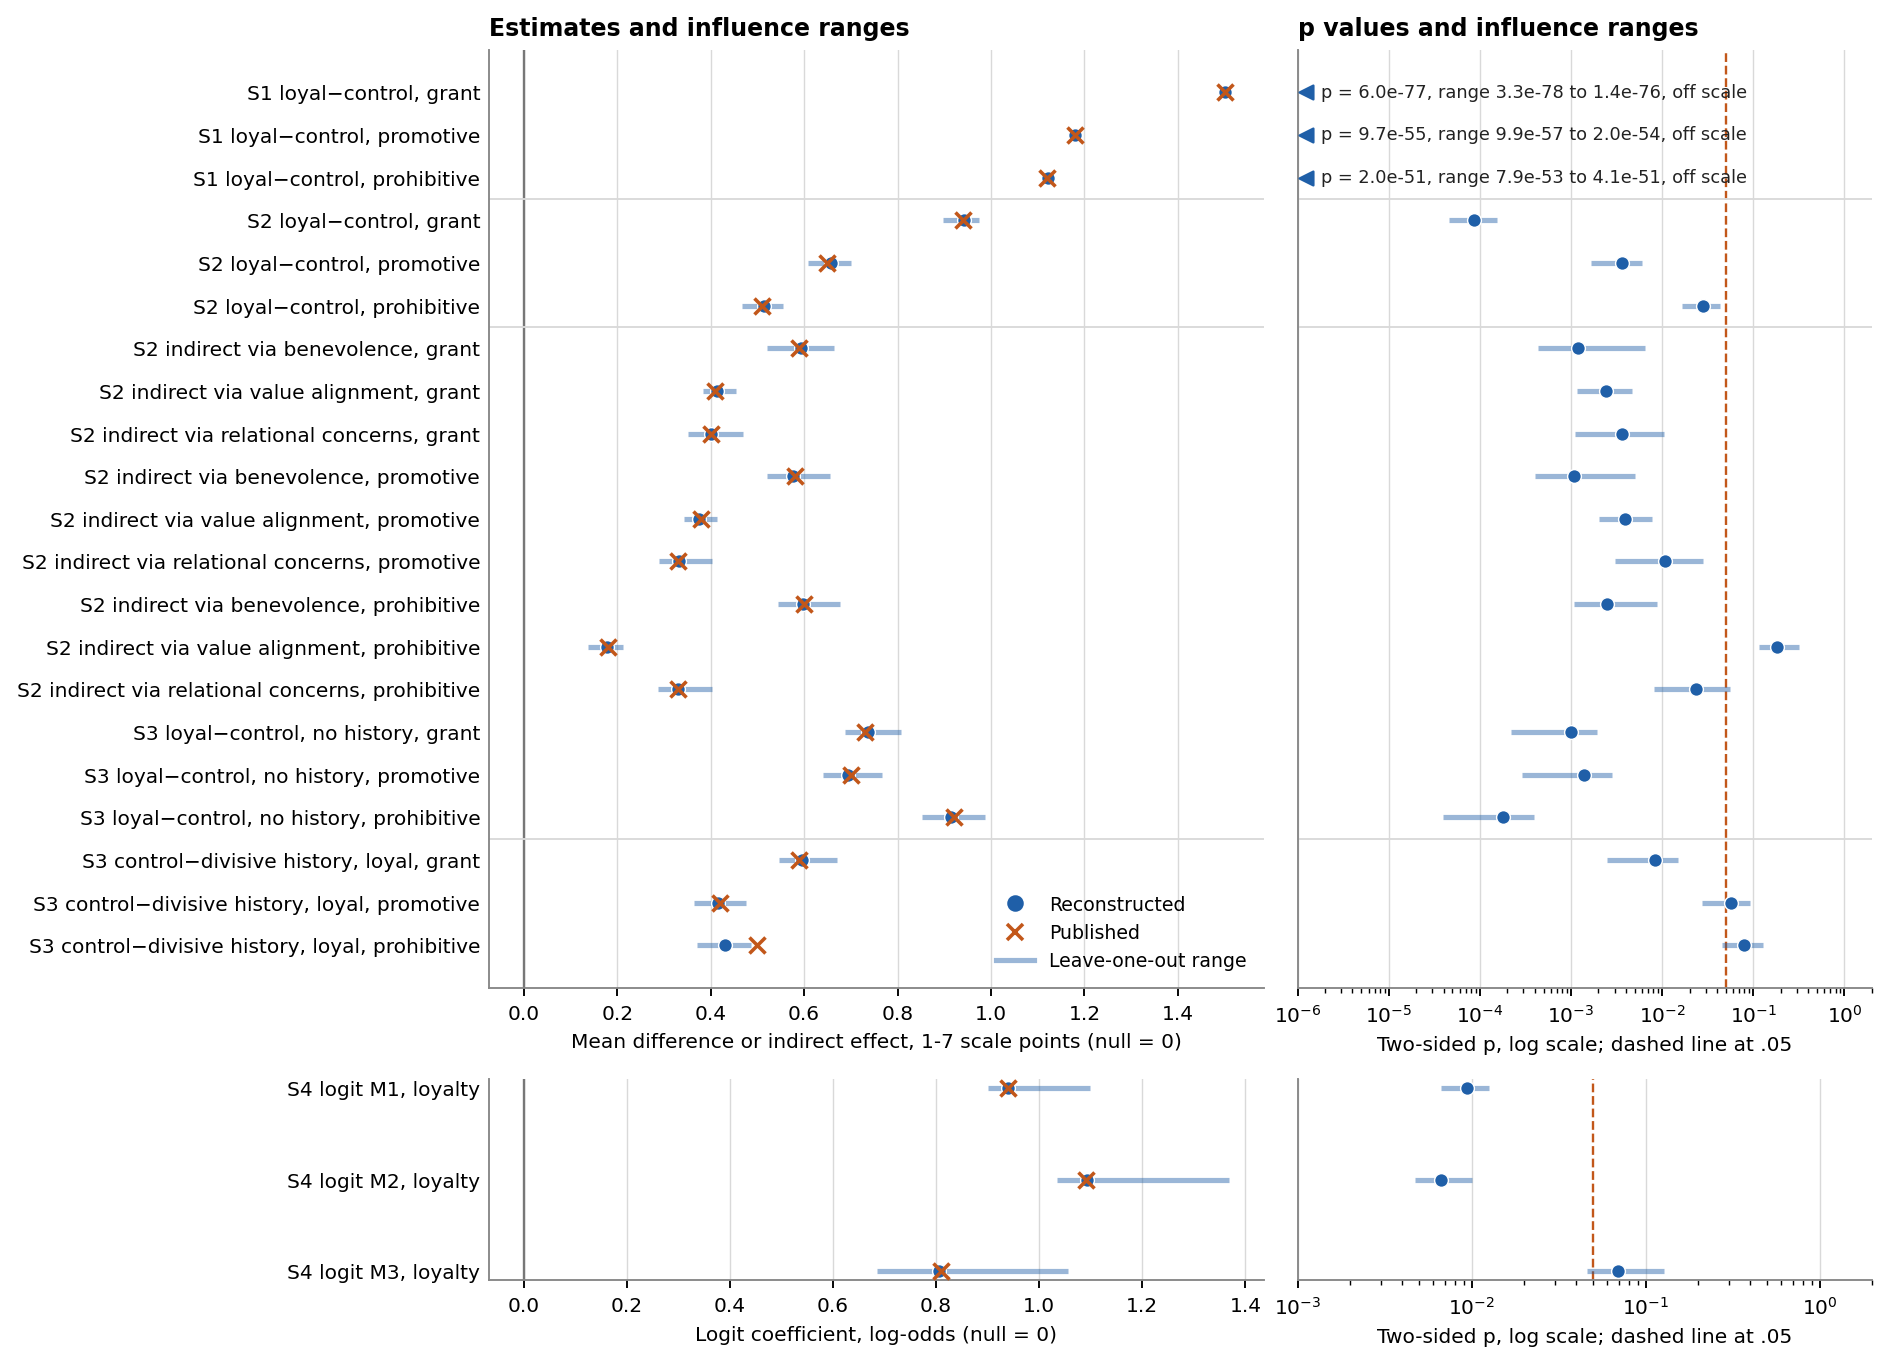
\includegraphics[width=\linewidth,height=.55\textheight,keepaspectratio]{supplement_assets/berry2025.png}\caption{Focal estimates in Studies 1--4 (left; mean differences and indirect effects in 1--7 scale points, logit coefficients in log-odds, null 0) and two-sided $p$-values (right, log scale). Crosses are published values, dots rebuilt values, lines the full leave-one-out range ($N=530$, 186, 286 and 50). Lines show influence ranges, not confidence intervals.}\label{fig:berry2025}\end{figure}
{\footnotesize Source: \artifact{studies/berry2025/reports/figures/reconstruction_influence.csv}.}

\textbf{Limits.} This is one paper from authors who shared voluntarily, with preregistrations and dictionaries, so it is likely a favorable case. The deposited data were processed by the authors, which removes the sample-reconstruction problem behind most gaps in the six public-source studies. The coordinator wrote the implementer manifest after seeing the published targets and the deposit's row counts; a leak scan found no target value in it. Memorization probes gave no sign of recall: Reader A weakly recognized the authors' research program and named no result, and Reader B recalled nothing. The adversarial review used Claude Opus 5.5, so no model family independent of both implementation families reviewed the result. The run took about two hours from authorization to the final report. One study does not generalize to experiments as a class.

\textbf{Evidence.} \artifact{studies/berry2025/reports/replication_report.md}, \artifact{reports/technical_supplement.md}, \artifact{reports/audit_pre_unseal.md}, \artifact{reports/adversarial_review.md}, \artifact{reports/exports/}, \artifact{logs/pre_unseal_hashes.json}, \artifact{logs/unseal_record.json}, and \artifact{runs/author_rerun/}. The article and the deposit are not redistributed; the deposit is at \url{https://osf.io/3h6vc}.

\clearpage
\section{Nagaraj (2021)}\label{sec:nagaraj}
\textbf{Overview and judgment.} Nagaraj (2021, \textit{Management Science} 67(8):4908--4934) studies how importing Census map data into OpenStreetMap affects subsequent contributions and map quality. This deposited-data reconstruction is separate from the six public-source cases and their common-rule comparison. The paper-level outcome is indeterminate under the study's frozen rules: of nine paper-focal claims, one is consistent, one has fragile inference, six are indeterminate, and one is discrepant but not fully verified. The discrepancy concerns the routing-error measure in Table 6. No human reviewed this run or its classifications; human verification remains a requirement before releasing a verified study report.

\textbf{Scope and inputs.} The run covered main-text Tables 1--7 and Figures 1--6, using the deposit at \url{https://osf.io/a47e9} and the Census TIGER/Line 2010 county file. All 60 deposit files matched the recorded OSF hashes; author code, the full Readme and the LaTeX results file remained sealed until the pre-unsealing record was hashed. These are author-processed aggregates, not a reconstruction from raw OpenStreetMap history. The deposit includes historical inputs that an outsider cannot independently reacquire in the same form, including Census correspondence, proprietary InfoUSA data and 2017 routing queries. Online Appendices A--D informed the methods but were outside the target set. Figure 1(b) was not audited because it is an illustrative image pair; the four Figure 3 panels were not scored because neither reader recorded numerical targets.

\textbf{Readers, implementation and access.} Independent readers received the article packet and data documentation without data rows. The coordinator reconciled their readings into an implementation manifest without published estimates or article identity. Separate implementers used Claude Opus 5.5 in R (A), GPT-6 Astra in R (B), and GPT-6 Astra in Python (C). They developed on synthetic files; the coordinator executed their frozen code on the empirical data with network access denied. Role processes used file-read barriers covering the project and session stores, but command-level internet access during development was controlled by instructions, not blocked. Astra's requested model and speed tier were not confirmed in its CLI receipts. The setup session had seen an earlier replication summary; its exposure was recorded, and the new research session used only the declared packet. The reader probes showed qualitative familiarity, so absence of prior knowledge cannot be established.

\textbf{Scoring and focal results.} The study used its own provisional, uncalibrated thresholds, not the post hoc common rule for the six cases. Magnitude was measured from the published rounding interval in published-SE units: at most 0.5 was a match, above 0.5 through 2 was grey, and above 2 was a mismatch. Inference used the $.01$, $.05$ and $.10$ thresholds. Sample gaps above 0.5\% prevented a consistent classification. Across all 84 ledger units, 17 were consistent, one had fragile inference, 53 were indeterminate, eight were discrepant but unverified, and five were not audited. The eight activity coefficients in Table~\ref{tab:nagaraj-focal} retain the published negative signs; seven remain significant at $.05$. This sign agreement does not resolve sample or magnitude differences.

% Generated by scripts/build_nagaraj_supplement_assets.py from frozen result exports.
\begin{table}[H]\centering\footnotesize
\setlength{\tabcolsep}{3pt}
\begin{tabularx}{\linewidth}{@{}>{\raggedright\arraybackslash}p{3.5cm}rrrY>{\raggedright\arraybackslash}p{2.3cm}@{}}\toprule
Claim & Published (SE) & Rebuilt (SE) & $p$ & $N$: published / rebuilt & Outcome\\\midrule
T3(3) Follow-on & $-0.1410$ (0.0484) & $-0.1215$ (0.0485) & 0.012 & 121,173 / 120,705 & Fragile inference\\
T3(4) Follow-on & $-0.1520$ (0.0448) & $-0.1047$ (0.0449) & 0.020 & 121,173 / 110,391 & Indeterminate\\
T3(5) Contributors & $-0.0557$ (0.0171) & $-0.0478$ (0.0171) & 0.005 & 121,173 / 120,705 & Consistent\\
T3(6) Contributors & $-0.0556$ (0.0143) & $-0.0433$ (0.0141) & 0.002 & 121,173 / 110,391 & Indeterminate\\
T4(3) Follow-on & $-0.1930$ (0.0604) & $-0.0796$ (0.0667) & 0.233 & 3,107 / 2,451 & Indeterminate\\
T4(4) Follow-on & $-0.4050$ (0.0657) & $-0.3181$ (0.0721) & $<.001$ & 3,107 / 2,451 & Indeterminate\\
T4(5) Contributors & $-0.1280$ (0.0166) & $-0.1238$ (0.0200) & $<.001$ & 3,107 / 2,451 & Indeterminate\\
T4(6) Contributors & $-0.2830$ (0.0186) & $-0.2705$ (0.0212) & $<.001$ & 3,107 / 2,451 & Indeterminate\\
T6(1) Routing error & $0.1260$ (0.0708) & $-0.1079$ (0.0333) & 0.001 & 81,007 / 80,370 & Discrepant, unverified\\
\bottomrule\end{tabularx}
\caption{Nagaraj (2021): nine paper-focal claims under the frozen study-specific rules.}\label{tab:nagaraj-focal}
\end{table}
{\footnotesize T3 denotes difference-in-differences models; columns 4 and 6 include controls. T4 denotes county cross-sections for 2008--2014 (columns 3 and 5) or 2014 (columns 4 and 6). T6 uses address pairs. Rebuilt SEs and two-sided $p$-values use county-clustered CR1 for T3 and T6, and HC1 for T4. Values are from the agreeing A--B implementation pair. Outcome labels also depend on sample reconstruction, printed-value consistency, and uncertain specifications, not only on the displayed coefficient and $p$-value. Unverified means the discrepancy survived review within the implementation model families but has not received independent-family or human verification.}


\textbf{Three comparisons.} The pre-unsealing hash record covered 391 files. The sealed author files matched their deposit hashes before and after opening. The comparisons below keep the frozen reconstruction separate from later diagnostics.
\begin{table}[H]\centering\small
\begin{tabularx}{\linewidth}{@{}p{.29\linewidth}Y@{}}\toprule
Comparison & Result\\\midrule
AI reconstruction against the article & Overall indeterminate; Table 6's focal routing-error coefficient reverses sign under the written absolute-error definition. No discrepancy has completed independent-family or human verification.\\
Author code against the article & Not run: Stata was unavailable. Inspection of the author code and modified AI scripts do not substitute for executing the original Stata pipeline.\\
AI code against author code & Inspection recorded 23 comparison items, including agreements and differences. Post-unsealing variants isolate sample, control-construction and outcome-definition choices. Applying the combined author choices brings the evaluated claims in Tables 3, 4, 5B and 7 within 0.36 published SEs. Frozen outcomes are unchanged.\\\bottomrule
\end{tabularx}\caption{Nagaraj (2021): reconstruction, unavailable author-code execution, and post-unsealing diagnostics.}\label{tab:nagaraj-comparisons}\end{table}

\textbf{The routing-error finding.} The article describes the logged absolute difference between OSRM and Google route lengths. All three implementations return a treatment coefficient of $-0.108$ under this definition (county-clustered SE $0.033$, $p=.0012$, $N=80{,}370$), against $0.126$ (SE $0.0708$, $N=81{,}007$) in Table 6, column 1. None of 35 uncertain alternatives meets the frozen pass criteria. Adversarial review retained the discrepancy, but used the same model family as implementation A. After unsealing, the author code was found to reverse the sign of the logged absolute error when the OSRM route is shorter. Adding this signed transformation alone to the frozen AI code gives $0.125$, close to the printed $0.126$. This is a diagnostic of a text--code difference, not a completed author-code rerun or a human-verified correction to the article.

\textbf{Other construction differences.} The author code retains Massachusetts as controls although the article says it is excluded, and interpolates and extrapolates county controls without describing those steps. The deposited ACS files end in 2011, whereas the article describes later years; 671 counties lack median earnings in the 2011 rows. The coordinator's fallback rule did not fill individual missing values, reducing the controlled panel to 110,391 observations and the cross-sections to 2,451 counties. That fallback is a limitation of this reconstruction. The author code also uses a window of twelve months either side of June 2005 for the timing sample, rather than the calendar years 2005--2006 stated in the article. Sample labels and some table headings are internally inconsistent, so several gaps remain classified as indeterminate.

\textbf{Uncertain specifications and influence.} Each implementation ran 1,295 grid rows: 112 origin settings, 530 single-axis deviations, 253 combinations of uncertain choices, and 400 placebo draws. These are three implementations of the same grid, not 3,885 distinct specifications. There were no alternatives jointly classified as equivalent, so specification fragility was not assessed. Implementation A completed 22,409 leave-one-county-out refits across the nine focal models; C repeated all of them with no failures and agreement on every refit. No deletion reversed a focal sign or crossed $.05$. Table 4, column 3 remained nonsignificant ($p=.18$--$.28$); the other eight focal coefficients remained significant.

\begin{figure}[H]\centering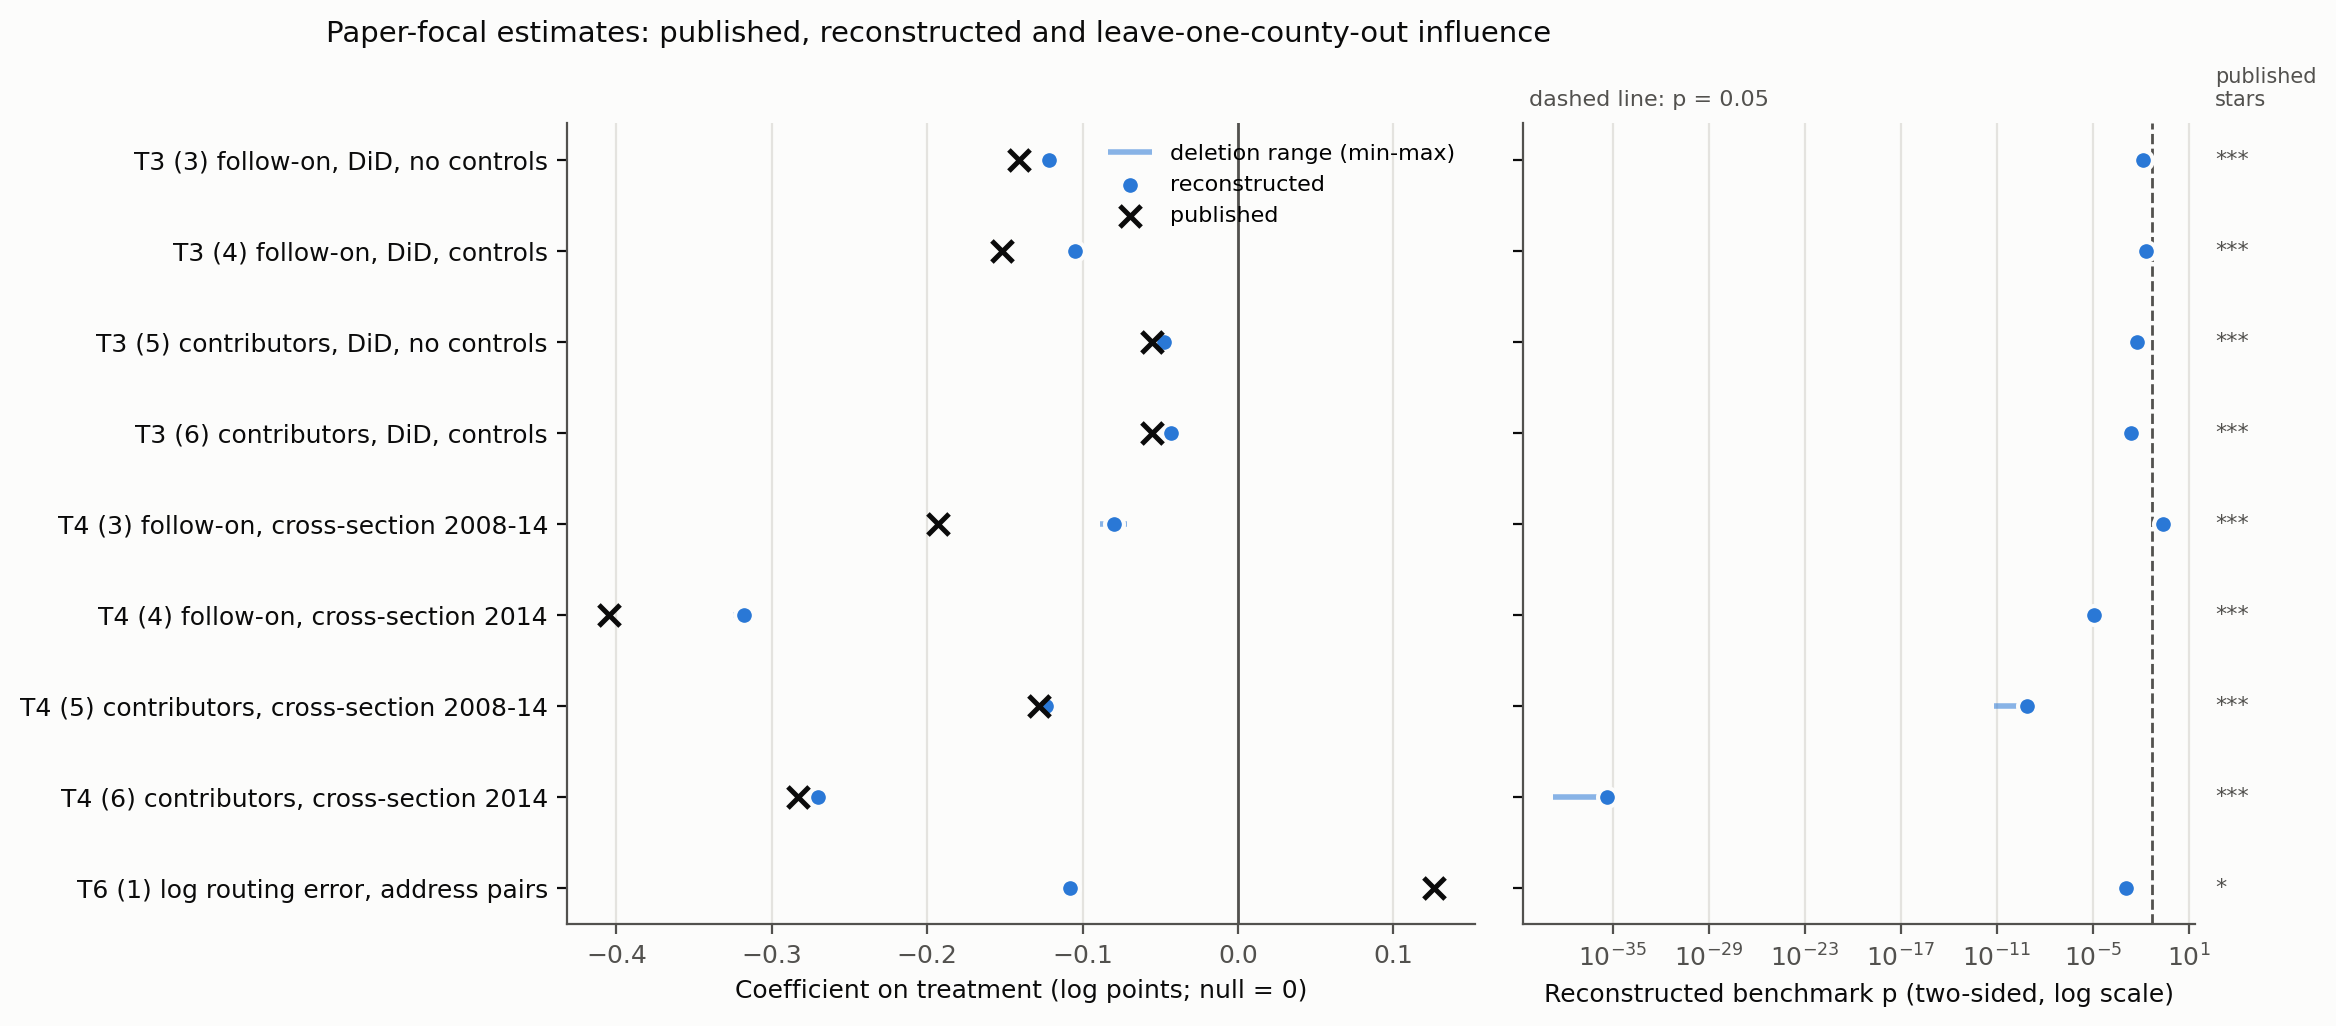
\includegraphics[width=\linewidth,height=.55\textheight,keepaspectratio]{supplement_assets/nagaraj2021.png}\caption{Nagaraj (2021): nine focal coefficients and leave-one-county-out influence. Crosses mark published coefficients; dots mark reconstructed coefficients (left) and two-sided benchmark $p$-values (right, log scale). Lines show deletion ranges, not confidence intervals. The dashed line marks $p=.05$; published significance stars appear at the right. Coefficients concern log activity counts or the logged routing-error measure. Table~\ref{tab:nagaraj-focal} reports numerical $p$-values and sample sizes.}\label{fig:nagaraj2021}\end{figure}
{\footnotesize Source: \artifact{supplement_assets/generated/nagaraj2021_influence.csv}, exported from the frozen run's \artifact{reports/figures/figure_focal_influence.csv}.}

\textbf{Figure diagnostics after unsealing.} The later comparison of Figure 6(a) found that the author's pooled regression without controls gives a top-decile follow-on coefficient of 1.075, against a published plot reading of 1.077. Separate per-decile models following the article's description instead give a near-zero or negative top-decile effect. The reported urban reversal therefore depends on the specification in this diagnostic. Visual comparison of Figure 2 suggests that the printed sample counts, rather than the map titles, were swapped; it is not a county-by-county verification. Annual aggregation brings the reconstructed Figure 3 series closer to the published display, but those panels remain unscored. These figure comparisons were added after unsealing and do not revise the frozen outcomes.

\textbf{Limits and retained evidence.} The case uses deposited aggregates, incomplete documentation, and a single study design. It cannot establish performance on raw-data reconstruction or generalize to natural experiments as a class. Scorer v1.1 corrected two omitted frozen rules before unsealing, without changing any outcome category; both versions are retained. No human review, independent-family discrepancy review, or author-code execution was completed. The source record is \artifact{studies/nagaraj2021/}: \artifact{reports/replication_report.md}, \artifact{reports/technical_supplement.md}, \artifact{reports/data/claim_outcomes.csv}, \artifact{scoring/scoring_rules_v1.json}, \artifact{runs/run_20261101_v1/scoring/final_summary.json}, \artifact{post_unseal/comparisons_2_and_3.md}, and \artifact{logs/pre_unseal_hashes.json}. The protocol as run is preserved under \artifact{studies/nagaraj2021/protocol_as_run/}. Source hashes for the table and figure are supplied in \artifact{supplement_assets/generated/nagaraj2021_provenance.json}.

\clearpage
\section{References and source record}
\begingroup\small\setlength{\parskip}{6pt}
Deephouse DL (1999) To be different, or to be the same? It's a question (and theory) of strategic balance. \textit{Strategic Management Journal} 20(2):147--166.

Delaney JT, Huselid MA (1996) The impact of human resource management practices on perceptions of organizational performance. \textit{Academy of Management Journal} 39(4):949--969.

Gartenberg C, Hasan S, Murray A, Pierce L (2026) More versus better: Artificial intelligence, incentives, and the emerging crisis in peer review. \textit{Organization Science} 37(3):795--812.

Holderness CG, Pontiff J (2012) Hierarchies and the survival of prisoners of war during World War II. \textit{Management Science} 58(10):1873--1886.

Kohler B, Zollikofer D, Einsiedler J, Hoyle A, Ash E (2026) Read the paper, write the code: Agentic reproduction of social-science results. arXiv:2604.21965. \url{https://arxiv.org/abs/2604.21965}.

Lehman DW, Hahn J, Ramanujam R, Alge BJ (2011) The dynamics of the performance--risk relationship within a performance period: The moderating role of deadline proximity. \textit{Organization Science} 22(6):1613--1630.

Liu S, Opsahl-Ong K, Drozdov A, Killingback J, Singhvi A, Pradeep R, Bendersky M, Dickerson JC, Lam MS (2026) AI-driven reproducibility and analytical robustness in scientific discovery. arXiv:2610.23845. \url{https://arxiv.org/abs/2610.23845}.

Nagaraj A (2021) Information seeding and knowledge production in online communities: Evidence from OpenStreetMap. \textit{Management Science} 67(8):4908--4934. \url{https://doi.org/10.1287/mnsc.2020.3764}.

Th\'ebaud S (2015) Business as plan B: Institutional foundations of gender inequality in entrepreneurship across 24 industrialized countries. \textit{Administrative Science Quarterly} 60(4):671--711.

Twenge JM, Campbell SM, Hoffman BJ, Lance CE (2010) Generational differences in work values: Leisure and extrinsic values increasing, social and intrinsic values decreasing. \textit{Journal of Management} 36(5):1117--1142.


Muravyev D (2026) Does empirical finance replicate? Working paper, University of Illinois Urbana-Champaign. \url{https://www.dmurav.com/replications/}.

Schwartz M, Andrews I, Shapiro JM (2026) An LLM workflow that reproduces, improves, and extends published economics research. NBER Working Paper 35782. \url{https://doi.org/10.3386/w35782}.
\endgroup
\end{document}
